% v17a: adds the exploratory n=4 (4,6) crossing 0.357 to Sec. n3annealed.
% v17 (annealed three-replica critical point): new Sec.~\ref{sec:n3annealed} with the
% exact sector-resolved spectra of C^{(3)} at L=4..12 (d=2) — p_c^{(3)}=0.305(3), a
% continuous transition with the three-state-Potts amplitude ratio and slope exponent,
% the n=2 control reproducing the deposited benchmark crossings, the growth-rate
% chain, and the lambda_1 simplicity observation; open-problems paragraph updated.
% v16 (recovered-data version), built from the ORIGINAL deposited v13 of the
% fuller_workspace release: the full audit-3 v14 plan (E1-E9, N3, D6, N2), the v15
% spinor factorisation, the authorised p_c re-centring 0.1595(10)->0.1597(8), and
% the end-to-end re-verification on the recovered raw dataset (seed contract 44/44
% bit-exact; released 1/N-floor pipeline reproduces every windowed number; the
% purification analysis reproduces every deposited number to the bit).
% Revised manuscript implementing audit_adjudication.md (Sept 2026).
% v8: certificate appendix (rank_audits_verification.md + qwen_open_verification.md surviving points).
% Original: uploads/manuscript_mipt_multifractality_rigorous.txt (unmodified).
% Change log: manuscript_revision_changelog.md
\documentclass[aps,prx,reprint,superscriptaddress,nobibnotes,longbibliography]{revtex4-2}
\usepackage{amsmath,amssymb,amsfonts,amsthm}
\usepackage{bm}
\usepackage{booktabs}
\usepackage{hyperref}
\usepackage{graphicx}

\newtheorem{theorem}{Theorem}
\newtheorem{proposition}{Proposition}
\newtheorem{lemma}{Lemma}
\newtheorem{corollary}{Corollary}
\newtheorem{definition}{Definition}
\newtheorem{conjecture}{Conjecture}
\theoremstyle{remark}
\newtheorem{remark}{Remark}
\newcommand{\id}{\operatorname{id}}
\newcommand{\Tr}{\operatorname{Tr}}
\newcommand{\Ran}{\operatorname{Ran}}
\newcommand{\Fix}{\operatorname{Fix}}
\newcommand{\HS}{\mathrm{HS}}
\newcommand{\E}{\mathbb E}
\newcommand{\cK}{\mathcal K}
\newcommand{\Wg}{\operatorname{Wg}}
\newcommand{\rk}{\operatorname{rank}}
\newcommand{\vth}{\vartheta}
\newcommand{\Ccomp}{\mathsf C_{\rm comp}}
\newcommand{\Tper}{\mathbb T_{\rm period}}
\newcommand{\Iv}[1]{\mathbf 1[#1]}

\begin{document}

\title{Exact Replica Mechanics and Born-Record Large Deviations in Monitored Quantum Circuits}
\author{Amin Abaee}
\thanks{ORCID: \href{https://orcid.org/0000-0002-0019-1842}{0000-0002-0019-1842}; Email: \href{mailto:abaee@ut.ac.ir}{abaee@ut.ac.ir}}
\affiliation{Independent Researcher}
\date{\today}

\begin{abstract}
We separate three structures that are often conflated in monitored-circuit calculations: linear outcome-summed replica channels, normalized conditional trajectories, and asymptotic large deviations.  For fixed-basis projective measurements we prove that the one-wire entanglement-feature span $\operatorname{span}\{I,S\}$ is not invariant; its minimal invariant unital algebra is $\operatorname{span}\{I,S,C\}$ with $C=\sum_m|mm\rangle\langle mm|$, and we give the leakage norm exactly for every replica number.  Nevertheless, when every measurement layer is followed by independently Haar-averaged two-site gates on a perfect matching and the system is sampled after the gate average, the $2^L$-dimensional feature space closes exactly; the analogous closure on the $n$-replica permutation span holds for all $n$ with an explicit Weingarten bond channel.  For every replica number the one-period operator is, on the range of its final gate average, of the form $\mathsf A\mathsf A^\dagger$ in the Hilbert--Schmidt inner product, so its nonzero spectrum is real, positive and semisimple, strictly inside the unit disk for every positive monitoring rate, with an $n!$-fold eigenvalue $1$ at $p=0$ and rank one at $p=1$; it commutes with a global $S_n\times S_n$ replica symmetry, and its nonzero spectrum compresses to the bond-label space.  For $n=2$ we derive the bond channel, state a proof-to-computation contract for the global transfer operator, and compress its nonzero spectrum to dimension $2^{L/2}$.  We prove that the compressed operator's rank is exactly $3\cdot2^{L/2-2}$ for every $p\in[0,1)$ and every $d$, strictly below the dimension $2^{L/2}$ of the compressed space.  For three replicas the rank depends on $p$: exact certificates over $\mathbb Z[p]$ give the generic rank---equal to the symmetry bound for $L\le10$ but $70$ below it at $L=12$, identically for every local dimension computed---the algebraic exceptional points at which it drops (all of them for $L\le8$), and the endpoint ranks.  The bond weight is shown to be exactly the anisotropic triangular-lattice Ising model of Bao, Choi and Altman, so the annealed two-replica model is exactly solvable: its growth rate is Houtappel's free energy and its critical point has the closed form $a-c=2b$, i.e.\ $p_c^{(2)}(d)=(d-\vth_c)/(d-1)$ with $\vth_c=\beta_d+\sqrt{\beta_d^2+1}$, $\beta_d=(d^2-1)/(d^2+1)$.  This exact solution benchmarks the transfer-matrix chain; its complete nonzero spectrum is obtained in closed free-fermion form, fixing the finite-size amplitudes at the annealed point exactly; and the annealed point is distinct from the quenched, Born-weighted transition, whose critical point an independent purification locator with disjoint seeds confirms.  For three replicas the annealed critical point is located by exact sector-resolved transfer-matrix scaling at $p_c^{(3)}=0.305(3)$ ($d=2$): the transition is continuous, with the amplitude ratio and slope exponent of the three-state Potts class rather than the Ising class of $n=2$, so the annealed replica points move away from the quenched transition as the replica number grows; the four-replica point, now resolved with full $S_4$ colour resolution at three sizes, continues the trend at $p_c^{(4)}=0.40$ with the marginal $q=4$-Potts scaling, and the first $n=5$ diagnostics steepen every sharpness measure as the first-order prediction requires.  We then distinguish symmetric unnormalized replica moments from the Born-weighted Mellin function; an information-theoretic counterexample proves that the former do not determine the quenched R\'enyi entropy, while the bivariate moment family does.  Conditional-trajectory decision is complete for PostBQP as a promise problem, hence PP-hard, for a precisely specified worst-case circuit family, and so is a conditional purity decision problem.  Finally, we replace a telescoping endpoint-entropy tilt by the time-additive surprisal of the Born record, derive sample-wise scaled-cumulant and multifractal identities under explicit large-deviation hypotheses, note that Clifford circuits have trivial record statistics, prove by an explicit random-energy construction that a Born-realizable sequence of record measures can have a finite-order freezing transition at $q_c=\sqrt{2\log2}$ that leaves the first derivative of the record scaled cumulant generating function continuous, specify a consistent sequential Monte Carlo estimator and convergence diagnostics, and run it: the first numerical quenched record SCGFs for Haar circuits, validated against exact enumeration, exhibit genuine record multifractality ($D(q)$ nonconstant) and bound the freezing transition away for $q\le3$ at $L\le12$.  Auxiliary-field statements are exact regulated identities or explicitly conditional effective-field-theory assumptions.
\end{abstract}

\keywords{monitored quantum circuits; measurement-induced transitions; replica transfer matrices; Weingarten calculus; triangular-lattice Ising model; exact rank certificates; Born-record large deviations; multifractality}

\maketitle

\section{Scope and conventions}

Monitored random circuits display measurement-induced entanglement transitions~\cite{Li2018,Skinner2019,Chan2019,Gullans2020,Choi2020,Vasseur2019,Jian2020,Bao2020}.  This work establishes exact finite-dimensional constraints on the replica mechanics underlying such transitions.  We prove statements that can serve as controlled inputs to later analytical and numerical studies: the fixed-basis replica leakage and its exact post-Haar closure, the two-replica transfer operator with its rank, its Ising structure and its closed-form annealed critical point, the spectral structure for every replica number and exact rank certificates for three replicas, Born-normalization identities, the worst-case complexity of conditional trajectories, and the large-deviation definitions for the Born record.  None of the exact results determines the quenched, Born-weighted transition: the critical point $p_c^{(2)}(d)$ of Sec.~\ref{sec:ising} is the known annealed two-replica Ising point~\cite{Bao2020,Houtappel1950}, and no logarithmic conformal field theory or replica-symmetry-breaking phase is derived.  Appendix~\ref{app:numerics} reports a separate, purely computational finite-size-scaling benchmark of the quenched transition for the Clifford realization of the same period (system sizes $16\le L\le512$, crossings, data collapse, bootstrap errors): $p_c=0.1595(10)$, $\nu=1.24(7)$, and critical half-chain entropy $S_{L/2}=\alpha\ln L+b$ with $\alpha=1.55(7)$ bits, i.e.\ $0.54(2)$ nats per cut; the quenched point lies $0.074$ below the exact annealed point $p_c^{(2)}(2)=0.2338$.  These numbers are consistent with the literature~\cite{Li2019,Zabalo2020,Sierant2022}; they are results of simulation, not theorems, and are quoted with systematic rather than statistical uncertainties.

A local wire has Hilbert space $H\cong\mathbb C^d$, $d\ge2$.  The two-replica one-wire space is $\cK=H^{\otimes2}$.  Superoperators act on column coordinate vectors, and products act from right to left.  We write $I=I_{\cK}$, $S$ for the replica swap, $P_m=|m\rangle\langle m|$, and
\begin{equation}
 C=\sum_{m=1}^d P_m^{\otimes2}=\sum_{m=1}^d|mm\rangle\langle mm|.
 \label{eq:Cdef}
\end{equation}
The fixed-basis outcome-correlated channel relevant to a linear two-replica outcome sum is
\begin{equation}
 \mathcal D(X)=\sum_{m=1}^dP_m^{\otimes2}X P_m^{\otimes2}.
 \label{eq:Ddef}
\end{equation}
The same outcome label appears in both replicas.  Equation~\eqref{eq:Ddef} is not independent-replica dephasing $\Delta^{\otimes2}$, which contains two independent outcome labels.  It is also not a normalized conditional update, which is nonlinear in the state.  Throughout, $p\in[0,1]$ is the per-site measurement probability, $n$ the replica number, $L$ the (even) number of sites, and
\begin{equation}
 \vth=d-(d-1)p\in[1,d]
 \label{eq:vth}
\end{equation}
the combination through which $p$ enters every two-replica formula.  The letter $q$ is reserved for the multifractal moment order of Sec.~\ref{sec:records}; the sans-serif $\mathsf K_R$ denotes a Kraus operator, $K_{\rm o/e}$ the matching factors of Sec.~\ref{sec:compression}, $K_{d,h}$ Ising couplings, and $K_\omega(x,dy)$ a Markov kernel.

\section{Exact two-replica lattice mechanics}

The coordinates of a replicated operator in the basis $\{I,S\}^{\otimes L}$ are the ``entanglement features'' of Ref.~\cite{Kuo2020}; we use that name for the span $\operatorname{span}\{I,S\}^{\otimes L}$.

\subsection{Fixed-basis leakage and its minimal algebra}

\begin{theorem}[Fixed-basis algebra and failure of local feature closure]
\label{thm:fixed-algebra}
The map $\mathcal D$ is the Hilbert--Schmidt orthogonal projector onto
\begin{equation}
 \mathfrak A_d=\operatorname{span}\{E_m=|mm\rangle\langle mm|:1\le m\le d\}.
\end{equation}
Thus $\Ran\mathcal D=\Fix\mathcal D=\mathfrak A_d$, an abelian $d$-dimensional $*$-algebra with unit $C$ on its support.  Moreover,
\begin{equation}
 \mathcal D(I)=\mathcal D(S)=\mathcal D(C)=C.
 \label{eq:DISC}
\end{equation}
For $d\ge2$, $\operatorname{span}\{I,S\}$ is not invariant.  The smallest unital $*$-subalgebra containing $I,S$ and invariant under $\mathcal D$ is
\begin{equation}
 \mathfrak B_d=\operatorname{span}\{I,S,C\}.
 \label{eq:Bd}
\end{equation}
\end{theorem}

\begin{proof}
Since $E_m$ is rank one,
$\mathcal D(X)=\sum_m\langle mm|X|mm\rangle E_m$.
The $E_m$ are pairwise Hilbert--Schmidt orthonormal idempotents, proving the projector, range, fixed-point, and algebra statements.  Since $E_mS=SE_m=E_m$, Eq.~\eqref{eq:DISC} follows.  The Gram matrix of $(I,S)$ is
\begin{equation}
 G_{IS}=\begin{pmatrix}d^2&d\\d&d^2\end{pmatrix},\qquad
 G_{IS}^{-1}=\frac1{d(d^2-1)}\begin{pmatrix}d&-1\\-1&d\end{pmatrix}.
\end{equation}
It gives
\begin{equation}
 \Pi_{IS}C=\frac{I+S}{d+1},\qquad
 \|C-\Pi_{IS}C\|_{\HS}^2=\frac{d(d-1)}{d+1}>0.
 \label{eq:leaknorm}
\end{equation}
Hence the often-used equality $C=(I+S)/(d+1)$ is false; the right-hand side is only the orthogonal projection.  Any invariant algebra containing $I,S$ contains $\mathcal D(I)=C$.  Conversely $S^2=I$, $C^2=C$, and $SC=CS=C$, so Eq.~\eqref{eq:Bd} is a unital invariant $*$-algebra and is minimal.
\end{proof}

For computations, the ordered nonorthogonal basis $(I,S,C)$ has
\begin{equation}
 G_{ISC}=\begin{pmatrix}d^2&d&d\\d&d^2&d\\d&d&d\end{pmatrix}\!,\ \ 
 G_{ISC}^{-1}=\tfrac{1}{d(d-1)}\!
 \begin{pmatrix}1&0&-1\\0&1&-1\\-1&-1&d{+}1\end{pmatrix}\!.
 \label{eq:GISC}
\end{equation}
For $\mathcal M_p=(1-p)\id+p\mathcal D$, column coordinates give
\begin{equation}
 [\mathcal D]_{ISC}=\begin{pmatrix}0&0&0\\0&0&0\\1&1&1\end{pmatrix},\quad
 [\mathcal M_p]_{ISC}=\begin{pmatrix}1{-}p&0&0\\0&1{-}p&0\\p&p&1\end{pmatrix}\!.
 \label{eq:MpISC}
\end{equation}
For arbitrary $X$, the orthogonal feature projection is
\begin{equation}
 \Pi_{IS}X=\alpha I+\beta S,\ \ 
 \binom\alpha\beta=\tfrac{1}{d(d^2-1)}\!
 \begin{pmatrix}d&-1\\-1&d\end{pmatrix}\!
 \binom{\Tr X}{\Tr(SX)}\!.
 \label{eq:PiIS}
\end{equation}
Applying Eq.~\eqref{eq:PiIS} after each measurement is an approximation, not an exact representation of Eq.~\eqref{eq:Ddef}.  Its size as an operator is exact: on $\operatorname{span}\{I,S\}$ with the Hilbert--Schmidt norm, the one-site defect $\Delta_p=\mathcal M_p-\Pi_{IS}\mathcal M_p=p(\id-\Pi_{IS})\mathcal D$ has operator norm
\begin{equation}
 \|\Delta_p\|_{\operatorname{span}\{I,S\}\to\cK\otimes\cK}=p\,\frac{\sqrt{2(d-1)}}{d+1},
 \label{eq:defectnorm}
\end{equation}
because $\Delta_p(\alpha I+\beta S)=p(\alpha+\beta)(C-\Pi_{IS}C)$ and $\sup|\alpha+\beta|/\|\alpha I+\beta S\|_{\HS}=\sqrt{2/(d(d+1))}$; the number $p\sqrt{d(d-1)/(d+1)}$ sometimes quoted is $\|\Delta_p(I)\|_{\HS}$, not a norm bound.

The statements above extend to every replica number.  Let $n\ge2$, let $U_\pi$ ($\pi\in S_n$) permute the replicas of $H^{\otimes n}$, $\mathcal G_n=\operatorname{span}\{U_\pi\}$, $C_n=\sum_mP_m^{\otimes n}$, and $\mathcal D_n(X)=\sum_mP_m^{\otimes n}XP_m^{\otimes n}$.

\begin{proposition}[General replica number]
\label{prop:general-n}
(i) $\mathcal D_n(U_\pi)=C_n$ for every $\pi$, and the smallest unital $*$-algebra containing $\mathcal G_n$ and invariant under $\mathcal D_n$ is $\mathcal G_n+\mathbb CC_n$.
(ii) The Hilbert--Schmidt projection of $C_n$ onto $\mathcal G_n$ and the leakage norm are
\begin{align}
 \Pi_nC_n&=\frac{\sum_{\pi\in S_n}U_\pi}{(d+1)(d+2)\cdots(d+n-1)},\nonumber\\
 \|C_n-\Pi_nC_n\|_{\HS}^2&=d\Bigl[1-\frac{n!}{(d+1)\cdots(d+n-1)}\Bigr],
 \label{eq:leak-n}
\end{align}
valid also for $d<n$, where the $U_\pi$ are linearly dependent.
(iii) For a gate bond, the $n$-fold Haar twirl $\mathcal E^{(n)}_{ij}$ is the Hilbert--Schmidt projector onto $\operatorname{span}\{U_\sigma\otimes U_\sigma:\sigma\in S_n\}$; hence $\mathcal G_n^{\otimes L}$ is invariant from one post-gate strobe to the next for every $n$, with bond coordinates
\begin{align}
 W_{p,n}(\pi\mid\mu,\nu)=\sum_{\sigma\in S_n}&\Wg_{d^2}(\pi^{-1}\sigma)\,
 \bigl[(1-p)d^{c(\sigma^{-1}\mu)}+pd\bigr]\nonumber\\
 &\times\bigl[(1-p)d^{c(\sigma^{-1}\nu)}+pd\bigr],
 \label{eq:Wpn}
\end{align}
where $c(\cdot)$ counts cycles, $\Wg_{D}$ is the Weingarten function of $U(D)$~\cite{Collins2003,CollinsSniady2006} (the inverse of the Gram matrix $D^{c(\sigma^{-1}\tau)}$ for $D\ge n$, its pseudo-inverse otherwise), and $\mu,\nu,\pi$ label the input and output permutation operators on the two wires.
\end{proposition}

\begin{proof}
(i) $U_\pi|m\cdots m\rangle=|m\cdots m\rangle$ gives $\mathcal D_n(U_\pi)=\sum_m\langle m\cdots m|U_\pi|m\cdots m\rangle P_m^{\otimes n}=C_n$; also $U_\pi C_n=C_nU_\pi=C_n$ and $C_n^2=C_n$, so $\mathcal G_n+\mathbb CC_n$ is a unital $*$-algebra invariant under $\mathcal D_n$, and any invariant algebra containing $I$ contains $\mathcal D_n(I)=C_n$.
(ii) By Schur--Weyl duality the orthogonal projector onto the commutant $\mathcal G_n$ is the Haar twirl $X\mapsto\int dU\,U^{\otimes n}XU^{\dagger\otimes n}$.  Applied to $P_m^{\otimes n}$ it gives $\int d\psi\,(|\psi\rangle\langle\psi|)^{\otimes n}=P_{\rm sym}/\binom{d+n-1}{n}$ with $P_{\rm sym}=\frac1{n!}\sum_\pi U_\pi$; summing over $m$ gives the first formula.  Since $\Pi_n$ is an orthogonal projection, $\|C_n-\Pi_nC_n\|^2=\|C_n\|^2-\langle C_n,\Pi_nC_n\rangle=d-\sum_\pi\Tr(C_nU_\pi)/[(d+1)\cdots(d+n-1)]$ and $\Tr(C_nU_\pi)=d$.
(iii) Under the identification $(H_i\otimes H_j)^{\otimes n}\cong(\mathbb C^{d^2})^{\otimes n}$, Schur--Weyl duality for $U(d^2)$ says that the commutant of $\{U^{\otimes n}:U\in U(d^2)\}$ is spanned by the replica permutations of $\mathbb C^{d^2}$, which are the operators $U_\sigma\otimes U_\sigma$, $\sigma\in S_n$.  The twirl $\mathcal E^{(n)}_{ij}$ is an average of Hilbert--Schmidt-unitary conjugations, hence self-adjoint, and it is idempotent by the invariance of Haar measure; its fixed points are exactly the operators commuting with every $U^{\otimes n}$.  It is therefore the Hilbert--Schmidt orthogonal projector onto $\mathcal V_n^{\rm b}=\operatorname{span}\{U_\sigma\otimes U_\sigma\}\subset\mathcal G_n\otimes\mathcal G_n$.  Closure: start from $X\in\mathcal G_n^{\otimes L}$; the site layer maps it into $\operatorname{End}(H^{\otimes n})^{\otimes L}$, and the gate layer applies $\mathcal E^{(n)}_{ij}$ on every bond of a perfect matching, so each bond factor of the output lies in $\mathcal V_n^{\rm b}$; since every site belongs to exactly one bond, the output lies in $\mathcal G_n^{\otimes L}$.  Coordinates: the orthogonal projection of a bond operator $X$ onto $\mathcal V_n^{\rm b}$ is $\sum_\pi y_\pi U_\pi\otimes U_\pi$ with $\mathsf Gy=t$, where $\mathsf G(\pi,\sigma)=\Tr[(U_\pi\otimes U_\pi)^\dagger(U_\sigma\otimes U_\sigma)]=(d^2)^{c(\pi^{-1}\sigma)}$ is the Gram matrix and $t_\sigma=\Tr[(U_\sigma\otimes U_\sigma)^\dagger X]$; for $d^2\ge n$, $\mathsf G$ is invertible with inverse $\Wg_{d^2}(\pi^{-1}\sigma)$~\cite{Collins2003,CollinsSniady2006}, and otherwise $t$ lies in the range of $\mathsf G$ and $y=\mathsf G^+t$ is a solution.  For $X=\mathcal M_p^{(n)}(U_\mu)\otimes\mathcal M_p^{(n)}(U_\nu)$ the trace factors over the two wires, $t_\sigma=\Tr[U_\sigma^\dagger\mathcal M_p^{(n)}(U_\mu)]\,\Tr[U_\sigma^\dagger\mathcal M_p^{(n)}(U_\nu)]$, and by (i)
\begin{align*}
 \Tr[U_\sigma^\dagger\mathcal M_p^{(n)}(U_\mu)]&=(1-p)\Tr U_{\sigma^{-1}\mu}+p\Tr(U_\sigma^\dagger C_n)\\
 &=(1-p)d^{c(\sigma^{-1}\mu)}+pd,
\end{align*}
because $\Tr U_\pi=d^{c(\pi)}$ and $\Tr(U_\sigma^\dagger C_n)=\sum_m\langle m\cdots m|U_{\sigma^{-1}}|m\cdots m\rangle=d$.  Substituting gives Eq.~\eqref{eq:Wpn}.
\end{proof}

For $n=3$, Eq.~\eqref{eq:leak-n} gives $\|C_3-\Pi_3C_3\|^2=d(d-1)(d+4)/[(d+1)(d+2)]$; for $n=2$ it reproduces Eq.~\eqref{eq:leaknorm} and Eq.~\eqref{eq:Wpn} reproduces Theorem~\ref{thm:strobe} below.  The $n$-replica transfer operator acts on $\mathcal G_n^{\otimes L}$, of dimension $(\dim\mathcal G_n)^L$ ($=n!^L$ for $d\ge n$; $\dim\mathcal G_3=5$ and $\dim\mathcal G_4=14$ at $d=2$); its general structure---real positive semisimple nonzero spectrum, strict contraction, symmetry, and compression---is established in Theorem~\ref{thm:general-n} below, after the $n=2$ case has been worked out in full.

\subsection{Exact post-gate stroboscopic closure}

Let a Haar gate $U\in U(d^2)$ act on neighboring physical wires $i,j$ and define its two-replica twirl
\begin{equation}
 \mathcal E_{ij}(X)=\int dU\,U^{\otimes2}X(U^\dagger)^{\otimes2}.
 \label{eq:Etwirl}
\end{equation}
Here the replica ordering is understood consistently so that the bond identity and global replica swap are $II$ and $SS$.

\begin{theorem}[Exact gate-to-gate feature dynamics]
\label{thm:strobe}
Suppose that (i) each site is independently subjected to $\mathcal M_p$, (ii) the next layer consists of independent Haar gates on a disjoint perfect matching, and (iii) the replicated operator is sampled immediately after the Haar average of that gate layer.  Then $\{I,S\}^{\otimes L}$ is invariant from one post-gate strobe to the next, although it is not invariant at the intermediate post-measurement time.

For one gate bond define
\begin{equation}
 \mathcal B_p=\mathcal E_{ij}\circ(\mathcal M_{p,i}\otimes\mathcal M_{p,j}).
 \label{eq:Bpdef}
\end{equation}
In the ordered bond feature basis $(II,IS,SI,SS)$,
\begin{equation}
 [\mathcal B_p]=
 \begin{pmatrix}
 a&b&b&c\\0&0&0&0\\0&0&0&0\\c&b&b&a
 \end{pmatrix},
 \label{eq:Bpmatrix}
\end{equation}
where, with $\vth=d-(d-1)p$,
\begin{equation}
 a=\frac{d^2\vth^2-1}{d^4-1},\qquad
 b=\frac{\vth}{d^2+1},\qquad
 c=\frac{d^2-\vth^2}{d^4-1}.
 \label{eq:abc}
\end{equation}
At $p=0$, $a=1,c=0,b=d/(d^2+1)$; at $p=1$, every column is $(II+SS)/(d^2+1)$.  For $0<p<1$ all three entries are positive, and
\begin{equation}
 a-c=\frac{\vth^2-1}{d^2-1},\qquad a+c=\frac{\vth^2+1}{d^2+1},\qquad \frac{b}{a+c}=\frac{\vth}{\vth^2+1}.
 \label{eq:abc-combos}
\end{equation}
\end{theorem}

\begin{proof}
By the two-copy Schur--Weyl commutant, or equivalently the second Haar moment~\cite{Collins2003}, $\mathcal E_{ij}$ is the Hilbert--Schmidt orthogonal projector onto $\operatorname{span}\{II,SS\}$.  Hence, with the bond dimension $d^2$,
\begin{equation}
 \mathcal E_{ij}(X)=\alpha_XII+\beta_XSS,
 \label{eq:twirlproj}
\end{equation}
with
\begin{equation}
 \binom{\alpha_X}{\beta_X}=
 \frac1{d^2(d^4-1)}\begin{pmatrix}d^2&-1\\-1&d^2\end{pmatrix}
 \binom{\Tr X}{\Tr(SSX)}.
 \label{eq:twirlproj-coef}
\end{equation}
For $Y_A=\mathcal M_p(A)$, Eq.~\eqref{eq:DISC} yields
\begin{equation}
\begin{array}{c|cc}
 &\Tr Y_A&\Tr(SY_A)\\ \hline
 A=I&d\vth&d\\ A=S&d&d\vth
\end{array}.
\label{eq:localtraces}
\end{equation}
For $X=Y_A\otimes Y_B$, both traces in Eq.~\eqref{eq:twirlproj-coef} factor.  Substitution gives Eqs.~\eqref{eq:Bpmatrix} and \eqref{eq:abc}.  The image on each bond lies in $\operatorname{span}\{II,SS\}$, and a perfect matching covers every site.  Tensoring the bond channels therefore maps the global feature space into itself.  Alternating the two matchings preserves the assertion at each post-gate strobe.
\end{proof}

The entries $(a,b,c)$ are the $n=2$ Weingarten data of the replica statistical models of Refs.~\cite{Jian2020,Bao2020}, here organised as a strobed transfer matrix; Sec.~\ref{sec:ising} makes the identification with the Ising model of Ref.~\cite{Bao2020} exact.

For a periodic even chain, let
\begin{equation}
 \mathbb B_{\rm odd}(p)=\bigotimes_{(ij)\in\mathcal G_{\rm odd}}\mathcal B_p^{(ij)},\qquad
 \mathbb B_{\rm even}(p)=\bigotimes_{(ij)\in\mathcal G_{\rm even}}\mathcal B_p^{(ij)},
\end{equation}
with $\mathcal G_{\rm odd}=\{(1,2),(3,4),\ldots,(L-1,L)\}$ and $\mathcal G_{\rm even}=\{(2,3),\ldots,(L,1)\}$.
If a period begins just after an even gate layer, the exact column update is
\begin{equation}
 v_{t+1}=\Tper(p)v_t,\qquad
 \Tper(p)=\mathbb B_{\rm even}(p)\mathbb B_{\rm odd}(p).
 \label{eq:period}
\end{equation}
Starting immediately after an even gate layer, the corresponding chronological sequence is ``measurements, odd gates, measurements, even gates.''  Equation~\eqref{eq:period} is therefore a gate-to-gate stroboscopic map; at either intermediate post-measurement time the replicated operator generally belongs to $\mathfrak B_d^{\otimes L}$, not the feature space.

An enlarged-basis implementation need not store a $9\times9$ gate table.  In the order $(I,S,C)$ define $\mathsf t=(d^2,d,d)$ and $\mathsf s=(d,d^2,d)$.  For $A,B\in\{I,S,C\}$,
\begin{equation}
 \mathcal E_{ij}(A\otimes B)=\alpha_{AB}II+\beta_{AB}SS,
\end{equation}
with
\begin{equation}
 \alpha_{AB}=\frac{d^2\mathsf t_A\mathsf t_B-\mathsf s_A\mathsf s_B}{d^2(d^4-1)},\qquad
 \beta_{AB}=\frac{-\mathsf t_A\mathsf t_B+d^2\mathsf s_A\mathsf s_B}{d^2(d^4-1)}.
 \label{eq:9col}
\end{equation}
Equations~\eqref{eq:MpISC} and \eqref{eq:9col} provide a full-space check of Eq.~\eqref{eq:Bpmatrix}.

\begin{remark}[Initial and terminal vectors; record-collision interpretation]
\label{rem:v0}
For a computational-basis product initial state, or for any pure product state if the period begins with a gate layer, the post-even-gate strobe vector is
\begin{equation}
 v_0=\bigotimes_{(ij)\in\mathcal G_{\rm even}}\frac{II+SS}{d^2(d^2+1)},
 \label{eq:v0}
\end{equation}
because a pure product state has unit trace and unit purity on each bond; for a non-basis product state preceded by a measurement layer the coefficients differ.  Let $\langle\mathrm{tr}|=(d^2,d)^{\otimes L}$ be the trace functional in the $(I,S)$ basis and $\langle\mathrm{tr}_A|$ the functional with $(d,d^2)$ on the sites of a region $A$ and $(d^2,d)$ elsewhere.  Since $v_t=\E_U\sum_R\tilde\rho_R^{\otimes2}$ with unnormalized conditional states $\tilde\rho_R$, $\Tr\tilde\rho_R=p_R$,
\begin{align}
 \bar Z_2(t)&=\E_U\sum_Rp_R(t)^2=\langle\mathrm{tr}|\Tper^tv_0\rangle,\nonumber\\
 \bar P_{2,A}(t)&=\E_U\sum_Rp_R(t)^2\Tr\rho_{A,R}^2=\langle\mathrm{tr}_A|\Tper^tv_0\rangle.
 \label{eq:collision}
\end{align}
$\bar Z_2(t)$ is the probability that two independent runs of the same circuit produce the same record.  The leading eigenvalue $\lambda_1$ of $\Tper$ is therefore the decay rate of the record-collision probability, and $\lambda_1<1$ for $p>0$ expresses the growth of the record entropy, not an entanglement property; equivalently $\log\lambda_1$ is the annealed record scaled-cumulant generating function of Sec.~\ref{sec:records} at $k=-1$ ($q=2$).  At $p=0$, $\lambda_1=1$ is doubly degenerate (all-$I$ and all-$S$ are both fixed).
\end{remark}

\subsection{Proof-to-computation contract}

Let $\Pi_{IS}$ be the one-wire Hilbert--Schmidt projector in Eq.~\eqref{eq:PiIS}.  On the ordered feature basis $(I,S)$, the projected one-site map $\widehat{\mathcal M}_p=\Pi_{IS}\mathcal M_p$ has the symmetric coordinate matrix
\begin{equation}
 [\widehat{\mathcal M}_p]_{IS}=(1-p)\begin{pmatrix}1&0\\0&1\end{pmatrix}
 +\frac{p}{d+1}\begin{pmatrix}1&1\\1&1\end{pmatrix}.
 \label{eq:projectedMsymmetric}
\end{equation}
This projection is exact in one restricted composition.  Indeed,
$\mathcal E_{ij}(\Pi_{IS}\otimes\Pi_{IS})=\mathcal E_{ij}$ because
$\operatorname{Ran}\mathcal E_{ij}=\operatorname{span}\{II,SS\}$ is contained in
$\operatorname{Ran}(\Pi_{IS}\otimes\Pi_{IS})$.  Consequently
\begin{equation}
 \mathcal E_{ij}(\mathcal M_{p,i}\otimes\mathcal M_{p,j})
 =\mathcal E_{ij}(\widehat{\mathcal M}_{p,i}\otimes
 \widehat{\mathcal M}_{p,j})
 \label{eq:projected-equivalence}
\end{equation}
on feature-space inputs.  The projected map is therefore exact when the complete site layer is immediately followed by the independently Haar-averaged gate layer on a perfect matching, and it is not an exact representation at the intermediate post-measurement time, after a partial matching, or without the subsequent Haar average.  Two objects are excluded by name below.  An \emph{exposed projected measurement layer} is an application of $\widehat{\mathcal M}_p^{\otimes L}$ whose output is read out, or acted on by anything other than the complete Haar-averaged matching, before the next gate average (for instance a terminal post-measurement strobe); its error per site is Eq.~\eqref{eq:defectnorm}.  A \emph{triangular one-site surrogate} is any one-site $(I,S)$ update whose coordinate matrix is triangular, such as the heuristic ``measurement fixes $I$ and maps $S\mapsto(1-p)S+(p/d)I$''; no such matrix equals Eq.~\eqref{eq:MpISC} or its symmetric projection Eq.~\eqref{eq:projectedMsymmetric}.

\begin{definition}[Authoritative spectral operator]
\label{def:operator-contract}
For even $L$, periodic boundary conditions, column basis $\{I,S\}^{\otimes L}$ in lexicographic bit order, and a post-even-gate initial strobe, the authoritative operator is Eq.~\eqref{eq:period}, whose bond action is exactly Eq.~\eqref{eq:Bpmatrix}.  It may be implemented either directly from that bond action or by the symmetric projected factorization in Eqs.~\eqref{eq:projectedMsymmetric}--\eqref{eq:projected-equivalence}, provided every projected site layer is immediately followed by the complete independently Haar-averaged gate matching.  No triangular one-site surrogate or exposed projected measurement layer is part of this definition.
\end{definition}

The definition fixes basis, boundary condition, multiplication order, and observation time.  A matrix-free implementation is accepted as an implementation of $\Tper$ only after the following finite tests.

\begin{proposition}[Necessary implementation checks]
\label{prop:checks}
An exact-arithmetic or tolerance-controlled implementation of Definition~\ref{def:operator-contract} must satisfy:
\begin{enumerate}
\item every local column agrees with Eqs.~\eqref{eq:Bpmatrix}--\eqref{eq:abc};
\item a direct bond implementation agrees with the symmetric projected factorization of Eq.~\eqref{eq:projected-equivalence};
\item the feature-space result agrees, for random input vectors at several small $L$, with the enlarged $(I,S,C)^{\otimes L}$ construction from Eqs.~\eqref{eq:MpISC} and \eqref{eq:9col};
\item the matrix-free action and its transpose agree with an explicitly assembled dense matrix and its transpose for small $L$;
\item $p=0$ and $p=1$ reproduce the limiting columns stated in Theorem~\ref{thm:strobe}, and the rank and spectral structure agree with Theorem~\ref{thm:rank} of Sec.~\ref{sec:compression};
\item every reported eigenpair $(\lambda,r)$ has the scale-free right residual
\begin{equation}
 \eta_R=\frac{\|\mathbb T r-\lambda r\|_2}
 {\|\mathbb T r\|_2+|\lambda|\,\|r\|_2}
 \label{eq:rightresidual}
\end{equation}
below a declared tolerance (with $0/0$ defined as zero only for the exact zero pair).  For a nonnormal spectral analysis, the analogous left residual $\eta_L$, the biorthogonal condition number
$\kappa_\lambda=\|\ell\|_2\|r\|_2/|\ell^\dagger r|$~\cite{StewartSun1990}, and the matching convention are also reported.  A small residual certifies a returned pair, not its claimed global modulus rank; that rank requires a full dense spectrum or a separately validated enclosure/selection argument.
\end{enumerate}
\end{proposition}

\begin{proof}
Item 1: by Definition~\ref{def:operator-contract} the bond action of the authoritative operator is Eq.~\eqref{eq:Bpmatrix} with the entries~\eqref{eq:abc}; an implementation whose local columns differ implements a different operator, and the comparison of four columns is a finite test.  Item 2: Eq.~\eqref{eq:projected-equivalence} is an identity of maps on feature-space inputs, so a direct bond implementation and the symmetric projected factorization must agree on every input; a discrepancy identifies an exposed projected layer or a triangular surrogate.  Item 3: the enlarged construction represents the site channel exactly, by Eq.~\eqref{eq:MpISC}, inside the invariant algebra $\mathfrak B_d^{\otimes L}$ of Theorem~\ref{thm:fixed-algebra}, and applies the exact twirl table~\eqref{eq:9col}; it never uses the bond matrix~\eqref{eq:Bpmatrix}, and on feature-space inputs its output equals $\Tper v$ by Theorem~\ref{thm:strobe}.  Agreement therefore checks the derivation of Eq.~\eqref{eq:Bpmatrix} as well as the code.  Item 4: the columns of the dense matrix are the images of the basis vectors under the matrix-free action, and an independent dense assembly from Kronecker products of Eq.~\eqref{eq:Bpmatrix} must reproduce them; the transpose is a separate code path and is needed for the left eigenvectors of item 6.  Item 5: the limiting columns are the $p=0$ and $p=1$ statements of Theorem~\ref{thm:strobe}; the rank $3\cdot2^{L/2-2}$, the reality and nonnegativity of the spectrum, the simplicity of $\lambda_1$ and the multiplicity $2^L-3\cdot2^{L/2-2}$ of the zero eigenvalue are Theorem~\ref{thm:rank}, each a finite test with a known answer.  Item 6: for a computed pair $(\lambda,r)$ the smallest perturbation $\delta\mathbb T$ (in the spectral norm) with $(\mathbb T+\delta\mathbb T)r=\lambda r$ exactly has norm $\|\mathbb Tr-\lambda r\|_2/\|r\|_2$, attained by $\delta\mathbb T=-(\mathbb Tr-\lambda r)r^\dagger/\|r\|_2^2$; $\eta_R$ is this backward error in scale-free form.  For a simple eigenvalue with left and right eigenvectors $\ell,r$ the first-order change under a perturbation is $\delta\lambda=\ell^\dagger\,\delta\mathbb T\,r/\ell^\dagger r$, so $|\delta\lambda|\le\kappa_\lambda\|\delta\mathbb T\|_2$~\cite{StewartSun1990}; the left residual certifies $\ell$ in the same way as $\eta_R$ certifies $r$.  A backward error bounds the distance of a returned pair from an exact pair of a nearby matrix and says nothing about eigenvalues that were not returned, which is why the global modulus rank requires the full spectrum or a separate enclosure.  Consequently, failure of any item prevents identification of the numerical object with the proved operator or of a numerical vector with its claimed eigenpair.
\end{proof}

\begin{proposition}[Approximate designs]
\label{prop:design}
Let every gate be drawn independently from a distribution $\nu$ on $U(d^2)$ whose two-replica twirl satisfies $\|\mathcal E_\nu-\mathcal E_{ij}\|_\diamond\le\varepsilon$ ($\varepsilon$-approximate unitary 2-design in diamond norm~\cite{Brandao2016}), and let $\mathbb T_\nu$ be the resulting one-period superoperator on two-replica operators.  Then
\begin{equation}
 \|\mathbb T_\nu-\Tper\|_\diamond\le L\varepsilon,
 \label{eq:designbound}
\end{equation}
with $(L/2)\varepsilon$ per matching layer and no higher-order term.  For $d=2$ and $\nu$ uniform on the two-qubit Clifford group, $\varepsilon=0$ and $\mathbb T_\nu=\Tper$ exactly~\cite{DiVincenzo2002}.
\end{proposition}

\begin{proof}
Write $\mathsf F_b=\mathcal E_{ij}\circ(\mathcal M_{p,i}\otimes\mathcal M_{p,j})$ and $\mathsf F_b^\nu=\mathcal E_\nu\circ(\mathcal M_{p,i}\otimes\mathcal M_{p,j})$ for the bond $b=(ij)$, each extended by the identity on the other sites, and number the $L$ bonds so that the odd matching comes first: $\Tper=\mathsf F_L\cdots\mathsf F_1$ and $\mathbb T_\nu=\mathsf F^\nu_L\cdots\mathsf F^\nu_1$, because factors within one matching act on disjoint sites and commute.  The telescoping identity
\begin{align*}
 &\mathsf F_L\cdots\mathsf F_1-\mathsf F^\nu_L\cdots\mathsf F^\nu_1\\
 &\qquad=\sum_{k=1}^{L}\mathsf F_L\cdots\mathsf F_{k+1}\,(\mathsf F_k-\mathsf F^\nu_k)\,\mathsf F^\nu_{k-1}\cdots\mathsf F^\nu_1
\end{align*}
is exact.  The diamond norm is submultiplicative, unchanged by tensoring with an identity map, and equal to $\|\Phi^*(\mathbb 1)\|_\infty$ for a completely positive map $\Phi$~\cite{Watrous2018}.  The twirls $\mathcal E_{ij}$ and $\mathcal E_\nu$ are mixtures of unitary conjugations, hence of diamond norm one; $\mathcal M_p$ is completely positive with $\mathcal M_p^*(\mathbb 1)=(1-p)\mathbb 1+pC\le\mathbb 1$ (the map $\mathcal D$ discards the off-diagonal replica blocks), so $\|\mathcal M_p\otimes\mathcal M_p\|_\diamond=\|\mathcal M_p^*(\mathbb 1)\otimes\mathcal M_p^*(\mathbb 1)\|_\infty\le1$.  Hence every $\mathsf F_b$ and $\mathsf F_b^\nu$ has diamond norm at most one, while $\|\mathsf F_b-\mathsf F_b^\nu\|_\diamond\le\|\mathcal E_{ij}-\mathcal E_\nu\|_\diamond\,\|\mathcal M_p\otimes\mathcal M_p\|_\diamond\le\varepsilon$.  The triangle inequality applied to the $L$ terms gives Eq.~\eqref{eq:designbound}, with $L/2$ terms, hence $(L/2)\varepsilon$, per matching layer; the identity is exact, so no higher-order term arises.  For the two-qubit Clifford group the second-moment operator equals the Haar one~\cite{DiVincenzo2002}, i.e.\ $\mathcal E_\nu=\mathcal E_{ij}$ and $\varepsilon=0$.  Note that $\mathbb T_\nu$ need not preserve the feature space; the bound is a statement on the full operator space, and the induced first-order shift of a simple eigenvalue, $|\delta\lambda|\le\kappa_\lambda\|\delta\mathbb T\|+O(\|\delta\mathbb T\|^2)$, must be evaluated with $\kappa_\lambda$ in a norm compatible with the one used for $\delta\mathbb T$.
\end{proof}

\begin{remark}[Clifford ensembles]
\label{rem:clifford}
Because two-qubit Cliffords form an exact 2-design, all annealed two-replica quantities of this section coincide for Haar and Clifford gates.  The quenched record statistics of Sec.~\ref{sec:records}, however, are trivial for Clifford circuits with stabilizer initial states and Pauli-basis measurements: whether a measurement outcome is deterministic or unbiased depends only on the unsigned stabilizer group, which evolves identically on every branch, so every record with positive probability has the same probability $2^{-N_{\rm rand}(\omega)}$, the surprisal $\mathcal A_T$ of Sec.~\ref{sec:records} is deterministic, and $\psi_{L,\omega}(k)$ is exactly linear in $k$.  Clifford circuits are therefore useless as a test bed for record multifractality, but they supply a free exact identity: $\E_\omega2^{-N_{\rm rand}(\omega)}=\bar Z_2(t)$ of Eq.~\eqref{eq:collision}, a cross-check between a stabilizer simulator and the transfer matrix (verified at $L=4$ to Monte Carlo accuracy, and at $L=16$, $p=0.16$, $t=2$ to four digits in Appendix~\ref{app:numerics}, Table~\ref{tab:numerics}).  The quenched entanglement transition of the Clifford ensemble is nontrivial, and Appendix~\ref{app:numerics} locates it numerically.
\end{remark}

\subsection{Nonzero-spectrum compression, rank, and spectral structure}
\label{sec:compression}

Since every local bond map has rank at most two, the first matching layer obeys $\rk\mathbb B_{\rm odd}\le2^{L/2}$, hence $\rk\Tper\le2^{L/2}$.  Theorem~\ref{thm:rank} below shows that this bound is never attained for $L\ge4$ and identifies the exact rank with a $p$- and $d$-independent combinatorial quantity.

The rank structure yields an exact spectral reduction.  Write the local bond matrix as
\begin{equation}
 [\mathcal B_p]=JK,\qquad
 J=\begin{pmatrix}1&0\\0&0\\0&0\\0&1\end{pmatrix},\qquad
 K=\begin{pmatrix}a&b&b&c\\c&b&b&a\end{pmatrix},
 \label{eq:JKfactor}
\end{equation}
and let $J_{\rm o/e}:\mathbb C^{2^{L/2}}\to\mathbb C^{2^L}$ and
$K_{\rm o/e}:\mathbb C^{2^L}\to\mathbb C^{2^{L/2}}$ be the tensor products on the odd/even matchings.  Define
\begin{equation}
 \Ccomp=K_{\rm e}J_{\rm o}K_{\rm o}J_{\rm e}=M_1M_2,\ \ M_1=K_{\rm e}J_{\rm o},\ M_2=K_{\rm o}J_{\rm e}.
 \label{eq:compressed}
\end{equation}
$J_{\rm o/e}$ are isometric embeddings and $K_{\rm o/e}$ are surjective whenever $a\ne c$, i.e.\ for $p<1$.

\begin{theorem}[Exact nonzero-spectrum compression]
\label{thm:compression}
With $N=2^L$ and $N_{\rm c}=2^{L/2}$,
\begin{equation}
 \det(\lambda I_N-\Tper)
 =\lambda^{N-N_{\rm c}}\det(\lambda I_{N_{\rm c}}-\Ccomp).
 \label{eq:charcompression}
\end{equation}
Consequently the nonzero eigenvalues, their algebraic multiplicities, and their nonzero Jordan elementary divisors agree.  If
$\Ccomp y=\lambda y$ with $\lambda\ne0$, then $J_{\rm e}y$ is a right eigenvector of $\Tper$.
\end{theorem}

\begin{proof}
The matching factorizations give
$\Tper=J_{\rm e}K_{\rm e}J_{\rm o}K_{\rm o}=\mathsf X\mathsf Y$
with $\mathsf X=J_{\rm e}$ and $\mathsf Y=K_{\rm e}J_{\rm o}K_{\rm o}$.  For $\lambda\ne0$ the block matrix $\begin{pmatrix}\lambda I_N&\mathsf X\\ \mathsf Y&I_{N_{\rm c}}\end{pmatrix}$ has the two Schur-complement determinants $\lambda^{N}\det(I_{N_{\rm c}}-\lambda^{-1}\mathsf Y\mathsf X)=\lambda^{N-N_{\rm c}}\det(\lambda I_{N_{\rm c}}-\mathsf Y\mathsf X)$ and $\det(I_{N_{\rm c}})\det(\lambda I_N-\mathsf X\mathsf Y)$; both are polynomials in $\lambda$, so they agree identically (Sylvester's determinant identity~\cite{Sylvester1851}; Ref.~\cite{HornJohnson2013}, Theorem~1.3.22).  With $\mathsf Y\mathsf X=\Ccomp$ this is Eq.~\eqref{eq:charcompression}, which identifies the nonzero eigenvalues together with their algebraic multiplicities.  The eigenvector lift follows by multiplying $\mathsf Y\mathsf Xy=\lambda y$ by $\mathsf X$.  For the Jordan data at $\lambda\ne0$ let $G_\lambda(\mathsf X\mathsf Y)=\ker(\mathsf X\mathsf Y-\lambda)^N$ be the generalized eigenspace.  If $x\in G_\lambda(\mathsf X\mathsf Y)$ and $\mathsf Yx=0$, then $(\mathsf X\mathsf Y)^jx=0$ for all $j\ge1$ and $0=(\mathsf X\mathsf Y-\lambda)^Nx=(-\lambda)^Nx$, so $x=0$: $\mathsf Y$ is injective on $G_\lambda(\mathsf X\mathsf Y)$, and $\mathsf Y(\mathsf X\mathsf Y-\lambda)^k=(\mathsf Y\mathsf X-\lambda)^k\mathsf Y$ shows that it maps $G_\lambda(\mathsf X\mathsf Y)$ into $G_\lambda(\mathsf Y\mathsf X)$ and intertwines the two restrictions.  The same argument with $\mathsf X$ gives the reverse injection, so $\mathsf Y$ restricts to an isomorphism $G_\lambda(\mathsf X\mathsf Y)\to G_\lambda(\mathsf Y\mathsf X)$ intertwining $\mathsf X\mathsf Y$ with $\mathsf Y\mathsf X$, and the Jordan blocks at $\lambda$ coincide in number and size (Flanders~\cite{Flanders1951}; Ref.~\cite{HornJohnson2013}, Theorem~3.2.11.1).  No similarity $\Tper\sim\Ccomp\oplus0$ is asserted at zero, where the block sizes of $\mathsf X\mathsf Y$ and $\mathsf Y\mathsf X$ may differ by one~\cite{Flanders1951}.
\end{proof}

Write the bond labels as Ising spins, $I\mapsto s=+1$ and $S\mapsto s=-1$, and let $m=L/2$.  The odd-bond labels $s=(s_1,\ldots,s_m)$ and the even-bond labels $s'=(s'_1,\ldots,s'_m)$ are cyclic, even bond $k$ lying between odd bonds $k$ and $k+1$.  Reading Eq.~\eqref{eq:Bpmatrix} column by column, the bond weight is
$\mathsf w(s'\mid s_1,s_2)=a$ if $s'=s_1=s_2$, $c$ if $s_1=s_2\ne s'$, and $b$ if $s_1\ne s_2$, so that
\begin{align}
 (M_1)_{s's}&=\prod_{k=1}^m\mathsf w(s'_k\mid s_k,s_{k+1}),\nonumber\\
 (M_2)_{s's}&=\prod_{k=1}^m\mathsf w(s'_k\mid s_{k-1},s_k).
 \label{eq:M1M2}
\end{align}
Call a bond $k$ of a label configuration $s$ a \emph{wall} if $s_k\ne s_{k+1}$, and let $\#(s)$ be the number of walls (always even).  Define the $2^m\times2^m$ zero--one matrix
\begin{equation}
 (V_m)_{s's}=\prod_{k=1}^m\bigl(\Iv{s_k\ne s_{k+1}}+\Iv{s_k=s_{k+1}=s'_k}\bigr),
 \label{eq:Vdef}
\end{equation}
which depends on neither $p$ nor $d$, and, for $0<p<1$, the numbers (the notation anticipates the Ising identification of Sec.~\ref{sec:ising})
\begin{equation}
 K_d=\tfrac14\log\tfrac ac>0,\ \ K_h=\tfrac14\log\tfrac{ac}{b^2}<0,\ \ \mathcal W_0=(acb^2)^{1/4}.
 \label{eq:Kdh}
\end{equation}
The signs follow from $a-c>0$, Eq.~\eqref{eq:abc-combos}, and from $b^2-ac=d^2(\vth^2-1)^2/[(d^2-1)^2(d^2+1)^2]>0$ for $\vth>1$.

\begin{theorem}[Rank and spectral structure of the compressed operator]
\label{thm:rank}
Let $L\ge4$ be even, $d\ge2$, and $m=L/2$.
\begin{enumerate}
\item[(i)] (Two factorizations.)  For $0\le p<1$, with $\mathsf Q=\begin{pmatrix}a&c\\c&a\end{pmatrix}$ in the $(I,S)$ basis and $\lambda_{\rm w}=b/(a+c)=\vth/(\vth^2+1)$,
\begin{equation}
 M_1=\mathsf Q^{\otimes m}\,V_m\,\operatorname{diag}\bigl(\lambda_{\rm w}^{\#(s)}\bigr).
 \label{eq:factorQ}
\end{equation}
For $0<p<1$, with $E_{s's}=\exp[K_d\sum_ks'_k(s_k+s_{k+1})]$ and $D_h=\operatorname{diag}(\exp[K_h\sum_ks_ks_{k+1}])$,
\begin{align}
 M_1&=\mathcal W_0^{\,m}\,E\,D_h,\qquad M_2=\mathcal W_0^{\,m}\,E^{\mathsf T}D_h,\nonumber\\
 \Ccomp&=\mathcal W_0^{\,L}\,E\,D_hE^{\mathsf T}D_h.
 \label{eq:Isingform}
\end{align}
\item[(ii)] (Similarity to a positive semidefinite matrix.)  For $0<p<1$, $\Ccomp=D_h^{-1/2}\bigl[\mathcal W_0^{L}\,\mathsf S\mathsf S^{\mathsf T}\bigr]D_h^{1/2}$ with $\mathsf S=D_h^{1/2}ED_h^{1/2}$.  Hence the spectrum of $\Ccomp$, and therefore the nonzero spectrum of $\Tper$, is real, nonnegative, and semisimple.  Moreover $\rk\Tper^2=\rk\Tper$, so the zero eigenvalue of $\Tper$ is semisimple as well: $\Tper$ is diagonalizable with real nonnegative spectrum for $0<p<1$.
\item[(iii)] (Perron--Frobenius.)  For $0<p<1$, $\Ccomp$ is entrywise positive.  Its largest eigenvalue $\lambda_1$ is simple with strictly positive left and right eigenvectors, strictly larger than every other eigenvalue, and $\langle\mathrm{tr}|J_{\rm e}y_1\rangle\,\langle\ell_1|K_{\rm e}J_{\rm o}v_0\rangle>0$ for the vectors of Remark~\ref{rem:v0}.  $\Ccomp$ commutes with the global relabeling $I\leftrightarrow S$; $y_1$ lies in the even sector.
\item[(iv)] (Exact rank.)  For $0\le p<1$,
\begin{equation}
 \rk\Tper=\rk M_1=\rk M_2=\rk V_m=3\cdot2^{m-2},
 \label{eq:rankexact}
\end{equation}
independent of $p$ and $d$; for $0<p<1$ also $\rk\Ccomp=3\cdot2^{m-2}$.  At $p=1$ the rank is one.
\item[(v)] (Kernel.)  $\ker M_1=\operatorname{diag}(\lambda_{\rm w}^{-\#(s)})\ker V_m$, so the null space is known for every $p$ once it is known for $V_m$.  $\dim\ker V_m=2^{m-2}$; every null vector of $V_m$ vanishes on the two uniform configurations and has parity $(-1)^{m+1}$ under the global flip $s\mapsto-s$.  For even $m$ the two all-wall configurations $s=(+,-,+,-,\ldots)$ and $-s$ have identical columns; for odd $m\ge3$, if $s^{(k)}$ denotes the configuration whose unique non-wall bond is $k$, then $e_{s^{(k)}}+e_{-s^{(k)}}-e_{s^{(j)}}-e_{-s^{(j)}}\in\ker V_m$ for $j\ne k$.
\end{enumerate}
\end{theorem}

\begin{proof}
(i) If $s_k\ne s_{k+1}$, the column $\mathsf w(\cdot\mid s_k,s_{k+1})=b(1,1)^{\mathsf T}=\lambda_{\rm w}\mathsf Q(1,1)^{\mathsf T}$ because $\mathsf Q(1,1)^{\mathsf T}=(a+c)(1,1)^{\mathsf T}$; if $s_k=s_{k+1}=s$, the column is $\mathsf Qe_s$.  Taking the tensor product over $k$ gives Eq.~\eqref{eq:factorQ}, the factor $\lambda_{\rm w}$ appearing once per wall.  For the Ising form one checks the three cases: $s'=s_1=s_2$ gives $\mathcal W_0e^{2K_d+K_h}=a$, $s_1=s_2\ne s'$ gives $\mathcal W_0e^{-2K_d+K_h}=c$, and $s_1\ne s_2$ gives $\mathcal W_0e^{-K_h}=b$, by Eq.~\eqref{eq:Kdh}; the horizontal factor $e^{K_hs_ks_{k+1}}$ depends only on the input row, which produces $D_h$, and the diagonal factors produce $E$.  Since $E_{ss'}=\exp[K_d\sum_ks_k(s'_k+s'_{k+1})]=\exp[K_d\sum_ks'_k(s_{k-1}+s_k)]$, the transpose $E^{\mathsf T}$ has exactly the structure of $M_2$ in Eq.~\eqref{eq:M1M2}.
(ii) $D_h$ is a positive diagonal matrix for $0<p<1$, so the displayed similarity is an algebraic identity from Eq.~\eqref{eq:Isingform}, and $\mathsf S\mathsf S^{\mathsf T}$ is real symmetric positive semidefinite.  Theorem~\ref{thm:compression} transfers the statement to the nonzero spectrum of $\Tper$.  For the zero eigenvalue, $\Tper=J_{\rm e}M_1K_{\rm o}$ and $\Tper^2=J_{\rm e}M_1M_2M_1K_{\rm o}$ with $J_{\rm e}$ injective and $K_{\rm o}$ surjective, while $M_1M_2M_1=\mathcal W_0^{3m}D_h^{-1/2}\,\mathsf S\mathsf S^{\mathsf T}\mathsf S\,D_h^{1/2}$ and $\rk(\mathsf S\mathsf S^{\mathsf T}\mathsf S)=\rk\mathsf S=\rk M_1$; hence $\rk\Tper^2=\rk\Tper$, so the Jordan blocks at zero have size one.
(iii) All products in Eq.~\eqref{eq:M1M2} are positive because $a,b,c>0$; the Perron--Frobenius theorem for positive matrices gives simplicity, positivity of the eigenvectors, and the strict gap.  The overlaps are positive because $v_0$, $\langle\mathrm{tr}|$, $J_{\rm e}$, $K_{\rm e}J_{\rm o}$ all have nonnegative and not identically vanishing coordinates against positive vectors.  The relabeling symmetry is that of Eq.~\eqref{eq:Bpmatrix} under $(II,IS,SI,SS)\mapsto(SS,SI,IS,II)$; a positive vector is even.
(iv) $\Tper=J_{\rm e}M_1K_{\rm o}$ with $J_{\rm e}$ injective and $K_{\rm o}$ surjective for $p<1$, so $\rk\Tper=\rk M_1$; $\mathsf Q$ is invertible because $a\ne c$ for $p<1$, and $\lambda_{\rm w}>0$, so $\rk M_1=\rk V_m$ by Eq.~\eqref{eq:factorQ}; $M_2$ is $M_1$ with its rows permuted by the cyclic shift $s'_k\mapsto s'_{k+1}$, so $\rk M_2=\rk M_1$.  For $0<p<1$, $\rk\Ccomp=\rk(\mathsf S\mathsf S^{\mathsf T})=\rk\mathsf S=\rk E=\rk M_1$.  At $p=1$, $a=c$ and every column of $[\mathcal B_p]$ coincides.  The value $\rk V_m=3\cdot2^{m-2}$ is Lemma~\ref{lem:rank} below.
(v) The first statement is Eq.~\eqref{eq:factorQ}.  The parity statement and $\dim\ker V_m=2^{m-2}$ are part of Lemma~\ref{lem:rank}.  For the uniform configurations, note that by Eq.~\eqref{eq:chartransform} below a vector $v$ lies in $\ker V_m$ iff the function $2^{\#(s)}v(s)$ is orthogonal to every $f_\Gamma$; the choices $\Gamma=\{1,\ldots,m\}$ and $\Gamma=\{1,\ldots,m\}\setminus\{j\}$ give $f_\Gamma=2^{|\Gamma|}(\delta_{s_+}\pm\delta_{s_-})$ with both signs (a ring cannot have exactly one wall), so $\delta_{s_\pm}$ lie in the span and $v(s_\pm)=0$.  Finally, an all-wall configuration has column $(1,1)^{\otimes m}$ of $V_m$, whence the even case; for odd $m$, the column of $s^{(k)}$ is $e_{\epsilon}$ at position $k$ ($\epsilon=s^{(k)}_k$) and $(1,1)^{\mathsf T}$ elsewhere, and summing over $\epsilon=\pm$ gives $(1,1)^{\otimes m}$ independently of $k$.
\end{proof}

\begin{lemma}[Rank of $V_m$]
\label{lem:rank}
For every $m\ge2$, $\rk V_m=3\cdot2^{m-2}$, $\dim\ker V_m=2^{m-2}$, and every vector in $\ker V_m$ has parity $(-1)^{m+1}$ under the global flip.
\end{lemma}

\begin{proof}
\emph{Step 1 (character transform).}  For $\Gamma\subseteq\{1,\ldots,m\}$ let $\chi_\Gamma(s')=\prod_{k\in\Gamma}s'_k$.  Multiplying Eq.~\eqref{eq:Vdef} by $\chi_\Gamma(s')$ and summing over $s'$ bond by bond, using $\sum_{s'_k}s'_k=0$ on wall bonds in $\Gamma$, $\sum_{s'_k}1=2$ on wall bonds outside $\Gamma$, $\sum_{s'_k}s'_k\Iv{s'_k=s_k}=s_k$ and $\sum_{s'_k}\Iv{s'_k=s_k}=1$ on non-wall bonds, gives
\begin{align}
 \sum_{s'}\chi_\Gamma(s')(V_m)_{s's}&=2^{\#(s)-|\Gamma|}f_\Gamma(s),\nonumber\\
 f_\Gamma(s)&=\prod_{k\in\Gamma}(s_k+s_{k+1}).
 \label{eq:chartransform}
\end{align}
The characters form an invertible transform of the row index and $2^{\#(s)}$ is an invertible column scaling, so $\rk V_m=\dim\operatorname{span}\{f_\Gamma\}$ in the $2^m$-dimensional space of functions on $\{\pm1\}^m$.

\emph{Step 2 (reduction to wall sets).}  Parametrize $s$ by its wall set $W$, an arbitrary subset of even cardinality, and by $\sigma=s_1$; then $s_k=\sigma(-1)^{|W\cap\{1,\ldots,k-1\}|}$.  $f_\Gamma(s)$ vanishes unless $\Gamma\cap W=\varnothing$, in which case $f_\Gamma(s)=2^{|\Gamma|}\prod_{k\in\Gamma}s_k$, so
\begin{align}
 f_\Gamma(s)&=2^{|\Gamma|}\sigma^{|\Gamma|}g_\Gamma(W),\nonumber\\
 g_\Gamma(W)&=\Iv{\Gamma\cap W=\varnothing}\,(-1)^{\sum_{w\in W}|\{k\in\Gamma:k>w\}|}.
 \label{eq:gGamma}
\end{align}
Functions with $|\Gamma|$ even are flip-even and those with $|\Gamma|$ odd are flip-odd, so the span splits into the two sectors, and within a sector $\sigma^{|\Gamma|}$ is a common factor.  Hence
\begin{align}
 \rk V_m=\dim\operatorname{span}\{g_\Gamma:|\Gamma|\equiv m\}&\nonumber\\
 +\dim\operatorname{span}\{g_\Gamma:|\Gamma|\not\equiv m\}&\pmod 2,
 \label{eq:sectorsum}
\end{align}
both spans being taken in the $2^{m-1}$-dimensional space of functions on even subsets $W$.

\emph{Step 3 (the sector $|\Gamma|\equiv m$ is full).}  Here $B=\Gamma^c$ is even, and $\Gamma\mapsto B$ is a bijection onto the even subsets.  By Eq.~\eqref{eq:gGamma}, $g_\Gamma(W)\ne0$ iff $W\subseteq B$, and $g_\Gamma(B)=\pm1$.  Ordering rows $B$ and columns $W$ by the same linear extension of inclusion (e.g.\ by cardinality), the $2^{m-1}\times2^{m-1}$ matrix $(g_\Gamma(W))_{B,W}$ is triangular with unimodular diagonal, hence invertible: the sector has dimension $2^{m-1}$.

\emph{Step 4 (the sector $|\Gamma|\not\equiv m$ has dimension $2^{m-2}$).}  Here $|\Gamma^c|$ is odd.  For every nonempty even set $\Lambda=\{c_1<\cdots<c_{2j}\}$ we claim
\begin{equation}
 \sum_{i=1}^{2j}(-1)^i\,g_{\Lambda^c\cup\{c_i\}}=0 .
 \label{eq:altrelation}
\end{equation}
Indeed, the $i$th term is nonzero at $W$ only if $W\subseteq\Lambda\setminus\{c_i\}$, and there its sign is $(-1)^{\sum_{w\in W}|\{k\in\Lambda^c:k>w\}|}$, common to all $i$, times $(-1)^{|\{w\in W:w<c_i\}|}$.  List the elements of $\Lambda\setminus W$ in increasing order; between two consecutive ones, $c_i<c_{i'}$, all $i'-i-1$ intermediate elements of $\Lambda$ belong to $W$, so the exponent $i+|\{w\in W:w<c_i\}|$ changes by $2(i'-i)-1$, an odd number.  The surviving terms therefore alternate in sign, and there is an even number of them ($|\Lambda\setminus W|=2j-|W|$), so they cancel.  Now let $|\Gamma|\not\equiv m$ with $m\in\Gamma$ and put $\Lambda=\Gamma^c\cup\{m\}$, an even set with $c_{2j}=m$ and $\Lambda^c\cup\{m\}=\Gamma$; relation~\eqref{eq:altrelation} expresses $g_\Gamma$ through the $g_{\Lambda^c\cup\{c_i\}}$, $i<2j$, none of which contains $m$.  Hence the sector is spanned by the $2^{m-2}$ functions $\{g_\Gamma:|\Gamma|\not\equiv m,\ m\notin\Gamma\}$.  These are linearly independent: for such $\Gamma$ the set $\Gamma^c$ is odd and contains $m$, so $W_\Gamma=\Gamma^c\setminus\{m\}$ is an even set; $g_{\Gamma'}(W_\Gamma)\ne0$ requires $W_\Gamma\subseteq\Gamma'^c$, i.e.\ $\Gamma^c\subseteq\Gamma'^c$ because both contain $m$, and $g_\Gamma(W_\Gamma)=\pm1$.  Ordering the $\Gamma$ by a linear extension of inclusion of the complements, the square matrix $(g_{\Gamma'}(W_\Gamma))_{\Gamma,\Gamma'}$ is triangular with unimodular diagonal.  So the sector has dimension exactly $2^{m-2}$.

\emph{Step 5.}  By Eq.~\eqref{eq:sectorsum}, $\rk V_m=2^{m-1}+2^{m-2}=3\cdot2^{m-2}$ and $\dim\ker V_m=2^{m-2}$.  For the parity, $V_m$ commutes with the flip, so it preserves the two flip eigenspaces $\mathcal E_\pm$, each of dimension $2^{m-1}$.  Rows of Eq.~\eqref{eq:chartransform} with $(-1)^{|\Gamma|}\ne\epsilon$ annihilate $\mathcal E_\epsilon$, and the remaining rows are, up to the invertible column scaling, the functions $f_\Gamma\in\mathcal E_\epsilon$ themselves; hence $\rk(V_m|_{\mathcal E_\epsilon})=\dim\operatorname{span}\{f_\Gamma:(-1)^{|\Gamma|}=\epsilon\}$, which by Steps 3--4 is $2^{m-1}$ for $\epsilon=(-1)^m$ and $2^{m-2}$ for $\epsilon=(-1)^{m+1}$.  Thus $V_m$ is injective on $\mathcal E_{(-1)^m}$ and $\ker V_m\subseteq\mathcal E_{(-1)^{m+1}}$.
\end{proof}

Theorem~\ref{thm:rank} corrects a natural but false expectation: entrywise positivity of $\Ccomp$ gives Perron--Frobenius, not invertibility, and $M_1$ is a surjection followed by an injection, which need not be invertible (at $L=4$ the columns $s=(+,-)$ and $(-,+)$ of $M_1$ coincide, so the rank is $3$).  For numerics the theorem is good news: the compressed operator can be restricted once and for all to a complement of the explicitly known, $p$-independent null space, and its spectrum can be obtained by a symmetric eigensolver applied to $\mathcal W_0^{L}\mathsf S\mathsf S^{\mathsf T}$.  The forced zero eigenvalue of $\Tper$ has algebraic and geometric multiplicity $2^L-3\cdot2^{L/2-2}$.  The rank values, the null-space parity, and the relations~\eqref{eq:altrelation} were also verified in exact arithmetic for $m\le11$.

\subsection{The two-replica model is an exactly solved Ising model}
\label{sec:ising}

Equation~\eqref{eq:Isingform} says that the strobed two-replica model is, exactly, the anisotropic Ising model on the triangular lattice with ferromagnetic coupling $K_d$ on the two diagonal directions (each even-bond spin couples to the two odd-bond spins below it, and vice versa) and antiferromagnetic coupling $K_h$ on the horizontal direction.  This is the $n=2$ replica model of Bao, Choi and Altman~\cite{Bao2020} (their Sec.~V.1; their weak-measurement angle corresponds to the projective rate through $\tan^4\alpha=p/(1-p)$, and their couplings are $J_d=-K_d\le0$, $J_h=-K_h\ge0$ in the convention $e^{-\beta H}$), whose critical point they located with Houtappel's solution~\cite{Houtappel1950}.  Its consequences for the transfer matrix are the following.

\begin{proposition}[Exact solution of the annealed two-replica model]
\label{prop:houtappel}
For $0<p<1$:
\begin{enumerate}
\item[(a)] The thermodynamic growth rate exists and equals $\lambda_\infty(p)=\lim_{L\to\infty}\lambda_1(L)^{1/L}=\mathcal W_0\,e^{f_{\rm H}(K_d,K_d,K_h)}$, where $f_{\rm H}$ is Houtappel's free energy per site of the triangular lattice~\cite{Houtappel1950,Baxter1982},
\begin{widetext}
\begin{align}
 f_{\rm H}(K_1,K_2,K_3)=\log2+\frac1{8\pi^2}\int_0^{2\pi}\!\!\int_0^{2\pi}d\theta_1d\theta_2\,
 \log\Bigl[&\cosh2K_1\cosh2K_2\cosh2K_3+\sinh2K_1\sinh2K_2\sinh2K_3\nonumber\\
 &-\sinh2K_1\cos\theta_1-\sinh2K_2\cos\theta_2-\sinh2K_3\cos(\theta_1+\theta_2)\Bigr].
 \label{eq:houtappel}
\end{align}
\end{widetext}
\item[(b)] $\lambda_\infty(p)$ is real-analytic in $p\in(0,1)$ except at the unique point where the bracket in Eq.~\eqref{eq:houtappel} vanishes at $\theta_1=\theta_2=0$, which in the variables of Theorem~\ref{thm:strobe} is the condition
\begin{align}
 a-c=2b\ \Longleftrightarrow\ \vth_c&=\beta_d+\sqrt{\beta_d^2+1},\quad \beta_d=\frac{d^2-1}{d^2+1},\nonumber\\
 p_c^{(2)}(d)&=\frac{d-\vth_c}{d-1}.
 \label{eq:pc2}
\end{align}
Numerically $p_c^{(2)}=0.233810$ ($d=2$), $0.459688$ ($d=3$), $0.594675$ ($d=4$), $0.679004$ ($d=5$), $0.846613$ ($d=10$); Eq.~\eqref{eq:pc2} is Eq.~(65) of Ref.~\cite{Bao2020} under $\tan^4\alpha_c=p_c/(1-p_c)$.
\item[(c)] The singularity is in the two-dimensional Ising universality class ($\nu=1$; scaling dimensions $x_\sigma=1/8$ for the $I\leftrightarrow S$-odd sector and $x_\epsilon=1$ for the leading even excitation).  For $p<p_c^{(2)}$ the model is ordered and the annealed quasi-entropy $\tilde S_2(A)=-\log[\bar P_{2,A}/\bar Z_2]$ of Eq.~\eqref{eq:collision}, which is the free energy of a domain wall terminating on $A$~\cite{Bao2020}, grows linearly in $|A|$ for $1\ll|A|\ll L$; for $p>p_c^{(2)}$ it saturates.
\end{enumerate}
\end{proposition}

\begin{proof}
(a) Let $m=L/2$.  By Eq.~\eqref{eq:Isingform}, $\Tr\,\Ccomp^{\,T}=\mathcal W_0^{LT}\,Z_{m,2T}$, where $Z_{m,2T}=\Tr(ED_hE^{\mathsf T}D_h)^T$ is the partition function of the Ising model on a periodic triangular lattice of $2T$ rows of $m$ spins: $E$ carries the $2m$ diagonal couplings $K_d$ between consecutive rows, $D_h$ the $m$ horizontal couplings $K_h$ within a row, so one period contains $L$ spins, $2L$ diagonal bonds and $L$ horizontal bonds, three bonds per spin; the factor $\mathcal W_0^{L}$ collects one $\mathcal W_0$ per bond factor $\mathsf w$ of the period.  By Theorem~\ref{thm:rank}(iii), $\lambda_1(L)$ is simple and strictly dominant, so $\lim_{T\to\infty}T^{-1}\log\Tr\,\Ccomp^{\,T}=\log\lambda_1(L)$, i.e.\ $\log\lambda_1(L)=L\log\mathcal W_0+2m\,f_m$ with $f_m=\lim_{T\to\infty}(2mT)^{-1}\log Z_{m,2T}$ the free energy per site of the periodic strip of width $m$.  For a finite-range interaction the free energy per site has a thermodynamic limit that does not depend on the shape of the domain or the order of the limits (Ref.~\cite{Ruelle1969}, Chap.~2), so $f_m\to f_{\rm H}(K_d,K_d,K_h)$ as $m\to\infty$, where $f_{\rm H}$ is Houtappel's closed form~\cite{Houtappel1950} for the anisotropic triangular lattice, Eq.~\eqref{eq:houtappel} (Ref.~\cite{Baxter1982}, Chap.~6, reaches the same lattice by the star--triangle transformation).  Hence $\lambda_1(L)^{1/L}\to\mathcal W_0e^{f_{\rm H}}$.

(b) Write $\mathsf s_d=\sinh2K_d>0$ and $\mathsf s_h=\sinh2K_h<0$.  From Eq.~\eqref{eq:Kdh}, $e^{2K_d}=\sqrt{a/c}$ and $e^{-2K_h}=b/\sqrt{ac}$, so
\begin{equation*}
 \mathsf s_d=\frac{a-c}{2\sqrt{ac}},\qquad |\mathsf s_h|=\frac{b^2-ac}{2b\sqrt{ac}},\qquad \mathsf s_de^{2K_h}=\frac{a-c}{2b}.
\end{equation*}
With $\cosh^22K_d=1+\mathsf s_d^2$, the bracket in Eq.~\eqref{eq:houtappel} at $\theta_1=\theta_2=0$ equals $e^{-2K_h}+\mathsf s_d^2e^{2K_h}-2\mathsf s_d=e^{-2K_h}(1-\mathsf s_de^{2K_h})^2=:\epsilon\ge0$, and the bracket minus its value at the origin is
\begin{equation*}
 \Delta(\theta_1,\theta_2)=\mathsf s_d(2-\cos\theta_1-\cos\theta_2)-|\mathsf s_h|\bigl(1-\cos(\theta_1+\theta_2)\bigr).
\end{equation*}
Since $|\sin(x+y)|\le|\sin x|+|\sin y|$ and $(u+v)^2\le2u^2+2v^2$, one has $1-\cos(\theta_1+\theta_2)=2\sin^2\frac{\theta_1+\theta_2}2\le2(1-\cos\theta_1)+2(1-\cos\theta_2)$, so $\Delta\ge0$ on the torus whenever $\mathsf s_d\ge2|\mathsf s_h|$.  By the displayed expressions this condition reads $b(a-c)\ge2(b^2-ac)$, and explicitly
\begin{equation*}
 b(a-c)-2(b^2-ac)=\frac{(\vth^2-1)\bigl[(d^4-1)\vth-2d^2\vth^2+2d^2\bigr]}{(d^2-1)^2(d^2+1)^2},
\end{equation*}
so for $\vth>1$ it is equivalent to $q(\vth)=2d^2\vth^2-(d^4-1)\vth-2d^2\le0$.  The quadratic $q$ is convex with $q(1)=-(d^4-1)<0$ and $q(d)=-d(d-1)^3(d+1)<0$, hence $q<0$ on all of $[1,d]$: $\mathsf s_d>2|\mathsf s_h|$ for every $0<p<1$.  Consequently the bracket is strictly positive on the whole torus except possibly at the origin, where it vanishes iff $\mathsf s_d=e^{-2K_h}$.  This is Houtappel's criticality condition $\mathsf s_d^2+2\mathsf s_d\mathsf s_h=1$ for this anisotropy pattern~\cite{Houtappel1950,Bao2020} (Ref.~\cite{Baxter1982}, Chap.~6), since $\mathsf s_d^2+2\mathsf s_d\mathsf s_h-1=(\mathsf s_d-e^{-2K_h})(\mathsf s_d+e^{2K_h})$ and the second factor is positive.  Away from such a point the integrand of Eq.~\eqref{eq:houtappel} is real-analytic in $(\vth,\theta_1,\theta_2)$ on the compact torus, so $f_{\rm H}$, and with it $\lambda_\infty=\mathcal W_0e^{f_{\rm H}}$, is real-analytic in $p$.  At such a point $f_{\rm H}$ is not analytic.  Indeed, $\mathsf s_de^{2K_h}=(a-c)/2b=(\vth-\vth^{-1})/2\beta_d$ increases strictly through $1$ at $\vth_c$, so $\epsilon(\vth)$ has a double zero there with $\epsilon''(\vth_c)>0$; near the origin $c_1|\theta|^2\le\Delta_\vth(\theta)\le c_2|\theta|^2$ with $c_1>0$, because the quadratic part $\frac12(\mathsf s_d-|\mathsf s_h|)(\theta_1^2+\theta_2^2)-|\mathsf s_h|\theta_1\theta_2$ of $\Delta$ is positive definite exactly when $\mathsf s_d>2|\mathsf s_h|$; and $\partial_\vth\Delta_\vth$, $\partial_\vth^2\Delta_\vth$ are $O(|\theta|^2)$.  Differentiating $\iint\log(\epsilon+\Delta_\vth)$ twice under the integral, every term stays bounded as $\vth\to\vth_c$ except $\epsilon''\iint d^2\theta/(\epsilon+\Delta_\vth)\ge\epsilon''(\pi/c_2)\log(1+c_2r^2/\epsilon)$, which diverges logarithmically: $\partial_\vth^2f_{\rm H}\to+\infty$ at $\vth_c$, Onsager's logarithmic specific heat in Houtappel's form~\cite{Houtappel1950}.  Finally, $\mathsf s_de^{2K_h}=1$ is $a-c=2b$; with Eq.~\eqref{eq:abc-combos} it reads $\vth^2-2\beta_d\vth-1=0$, whose positive root is $\vth_c=\beta_d+\sqrt{\beta_d^2+1}$, and $\vth_c\in(1,d)$ because $(a-c)/2b$ increases strictly from $0$ at $\vth=1$ to $(d^2+1)/2d>1$ at $\vth=d$.

(c) Flipping the spins of every other row reverses the sign of both diagonal couplings and leaves $K_h$ unchanged, so the model is gauge equivalent to the fully antiferromagnetic anisotropic triangular lattice whose two strongest couplings lie on the diagonals ($K_d>|K_h|$ follows from $\mathsf s_d>2|\mathsf s_h|$).  The triangular-lattice Ising model is a free-fermion (Pfaffian) model for every sign pattern of its couplings, and its exact pair correlations are Stephenson's~\cite{Stephenson1964,Stephenson1970}: for the anisotropic antiferromagnetic lattice there is a single transition, at Houtappel's point, below which the two strong axes carry antiferromagnetic and the weak axis ferromagnetic long-range order---in the original gauge, uniform order of the bond labels---and the correlation length diverges as $|\vth-\vth_c|^{-1}$ ($\nu=1$).  The specific heat is logarithmic by (b) ($\alpha=0$), and the long-range order vanishes with the exponent $\beta=1/8$ of the anisotropic triangular lattice~\cite{Potts1952,Stephenson1970}.  In the language of the $c=1/2$ Ising field theory, $x_\sigma=\beta/\nu=1/8$ and $x_\epsilon=2-1/\nu=1$; Table~\ref{tab:benchmark} confirms the ratio $x_\sigma/x_\epsilon$ numerically for the present sign pattern.  The $I\leftrightarrow S$ flip is the spin-reversal symmetry, so the flip-odd sector carries $x_\sigma$ and the leading flip-even excitation $x_\epsilon$.  The ordered phase is the small-$p$ side, because $K_d=\frac14\log(a/c)\to\infty$ as $p\to0$, consistent with the twofold degeneracy of $\lambda_1$ at $p=0$ (Remark~\ref{rem:v0}).  Finally, $\langle\mathrm{tr}_A|$ pairs the final row with the label $S$ on $A$ and $I$ elsewhere (Remark~\ref{rem:v0}), so $\bar P_{2,A}/\bar Z_2$ is the ratio of the partition functions with and without a domain wall forced to terminate at the two ends of $A$; in the ordered phase the wall costs a surface tension per unit length and $\tilde S_2(A)$ grows linearly in $|A|$ for $1\ll|A|\ll L$, while in the disordered phase the boundary condition is forgotten beyond a correlation length and $\tilde S_2(A)$ saturates~\cite{Bao2020}.
\end{proof}

Two remarks on interpretation.  First, $p_c^{(2)}$ is a singularity of the \emph{annealed} quantity $-\lim(tL)^{-1}\log\bar Z_2$, the record-collision (or annealed $q=2$ record) free energy.  It is distinct from the Born-weighted transition, which is not an $n=2$ quantity: for Haar qubit circuits it lies near $p_c\approx0.17$~\cite{Zabalo2020}, and for the Clifford realization of the present period Appendix~\ref{app:numerics} finds $p_c=0.1597(8)$, against $p_c^{(2)}(2)=0.2338$; at every size the quenched half-chain entropy lies strictly below the annealed quasi-entropy $\tilde S_2$, whose record-collision weight lowers the effective measurement density to $p_{\rm eff}=0.092$ at $p=0.16$ (Appendix~\ref{app:numerics}, Table~\ref{tab:numerics}), and at $p=0.22<p_c^{(2)}$ the quenched chain is already in its area-law phase while the annealed model is still ordered.  Second, the exact solution gives the transfer-matrix chain of Sec.~\ref{sec:compression} something rare: an end-to-end check with known answers.  Table~\ref{tab:benchmark} reports such a check, produced with a matrix-free implementation of $\Ccomp$ (sector-projected Arnoldi on $2^{L/2}$ states).  The finite-size crossings of the scaled $I\leftrightarrow S$ gap $L\log(\lambda_1/\lambda_{\rm odd})$ converge to Eq.~\eqref{eq:pc2} from below, the ratio of the odd and even gaps at $p_c^{(2)}$ approaches $x_\sigma/x_\epsilon=1/8$ (the lattice anisotropy cancels in the ratio), and $\lambda_1(L)^{1/L}$ agrees with Eq.~\eqref{eq:houtappel} to $3\times10^{-7}$ at $L=28$ and is certified exactly at rational points by the Collatz--Wielandt enclosures of Appendix~\ref{app:enclosures} ($d=2$, $p=0.40$: $0.6838449$ versus $0.6838447$).  At $d=2$, $L=32$ the annealed quasi-entropy $\tilde S_2(A)$ evaluated in the Perron state at $|A|=4$ and $8$ is $2.13,\,3.74$ ($p=0.12$), $1.77,\,2.85$ ($p=0.18$), $0.89,\,1.07$ ($p=0.30$) and $0.49,\,0.52$ ($p=0.40$): growth with $|A|$ below and saturation above $p_c^{(2)}$, as Proposition~\ref{prop:houtappel}(c) requires.  These data validate the proof-to-code chain against an exact solution.

\begin{table*}[t]
\caption{Benchmark of the compressed transfer matrix against the exact Ising solution.  $p^*(L_1,L_2)$: crossing of $L\log(\lambda_1/\lambda_{\rm odd})$ for consecutive sizes.  Ratio: $\log(\lambda_1/\lambda_{\rm odd})/\log(\lambda_1/\lambda_{{\rm even},2})$ at $p=p_c^{(2)}(d)$, to be compared with $x_\sigma/x_\epsilon=1/8$.}
\label{tab:benchmark}
\begin{ruledtabular}
\begin{tabular}{lcccccc}
 & $(16,20)$ & $(20,24)$ & $(24,28)$ & $(28,32)$ & exact & \\
\colrule
$p^*$, $d=2$ & 0.23319 & 0.23348 & 0.23361 & 0.23368 & 0.233810 & \\
$p^*$, $d=3$ & 0.45934 & 0.45950 & 0.45957 & 0.45961 & 0.459688 & \\
\colrule
 & $L=16$ & $L=20$ & $L=24$ & $L=28$ & $L=32$ & exact \\
\colrule
ratio, $d=2$ & 0.1220 & 0.1231 & 0.1237 & 0.1240 & 0.1243 & 0.125 \\
ratio, $d=3$ & 0.1232 & 0.1238 & 0.1242 & 0.1244 & 0.1245 & 0.125 \\
\end{tabular}
\end{ruledtabular}
\end{table*}

Because $\Tper$ is not normal in the coordinate inner product, a nonsymmetric Arnoldi method, Schur method, or dense diagonalization is appropriate on the full space; on the compressed space Theorem~\ref{thm:rank}(ii), or the Gram-metric form of Theorem~\ref{thm:general-n}(i) in Sec.~\ref{sec:general-n} below, allows a symmetric solver.  A one-vector power iteration is not Lanczos and does not in general certify the subleading eigenvalue.  The compression in Theorem~\ref{thm:compression} provides an independent full-spectrum route on $2^{L/2}=\sqrt{2^L}$ states.  Any correlation length defined from eigenvalues must state the selected eigenvalue, the symmetry sector, observable coupling, and degeneracy treatment.  The released small-size benchmarks ($L=4,6$, $d=2$, $p\in\{0.01,0.118,0.5\}$) obtain global ranks from the complete dense spectrum of $\Tper$, check it against the complete compressed spectrum (agreement to $4\times10^{-16}$, including the forced zero multiplicity $2^L-3\cdot2^{L/2-2}$), and cross-check the leading three eigenpairs with two-seed full-space Arnoldi, right and left residuals below $2\times10^{-15}$, and biorthogonal condition numbers $\kappa_\lambda\in[1.3,4.7]$.  All eighteen released eigenvalues are real and positive, the nonzero counts are $3$ and $6$, and at $L=6$ the fourth and fifth eigenvalues form an exact doublet carried by the two nonzero momenta of the three-site cyclic shift of the bond labels, all as Theorem~\ref{thm:rank} requires.  The released small-size benchmarks validate the proof-to-code chain; they are not a finite-size-scaling data set.  The crossings and gap ratios of Table~\ref{tab:benchmark} concern the exactly solved annealed model, whose transition point is known in closed form, and no quenched exponent or transition point is inferred from any of these data.


\begin{proposition}[closed form of the nonzero spectrum]
\label{prop:spectrum}
Let $L=2m\ge4$, $d\ge2$, $0<p<1$, and let $\Ccomp=\mathcal W_0^{\,L}ED_hE^{\mathsf T}D_h$ be the compressed period operator of Eq.~\eqref{eq:Isingform}, with $K_d,K_h,\mathcal W_0$ as in Eq.~\eqref{eq:Kdh}.  For $k\in[0,2\pi)$ define
\begin{equation}
 Q(k)=\cosh^2\!2K_d\,\cosh 2K_h+\sinh^2\!2K_d\,\sinh 2K_h-\sinh 2K_h\,\cos k,\qquad
 R(k)=2\sinh 2K_d\,\cos\tfrac{k}{2},
 \label{eq:QRdef}
\end{equation}
and $w_k^{\pm}=Q(k)\pm\sqrt{Q(k)^2-R(k)^2}$ (real, since $0\le R^2\le Q^2$ for all $k$).  Then every nonzero eigenvalue of $\Ccomp$ is of the form
\begin{equation}
 \lambda=\bigl(2\mathcal W_0^{\,2}\bigr)^m\prod_{k\in\mathcal K_\sigma}w_k^{\pm_k},
 \label{eq:spectrum}
\end{equation}
the product running over the momentum states of the flip sector $\sigma$: in the flip-even sector $\mathcal K_+=\{(2j-1)\pi/m:\ j=1,\dots,m\}$ (antiperiodic) with an \emph{even} number of ``$-$'' choices; in the flip-odd sector $\mathcal K_-=\{2\pi j/m:\ j=0,\dots,m-1\}$ (periodic) with an even number of ``$-$'' choices below $p_c^{(2)}(d)$ and an odd number above (the $k=0$ mode changes its branch ordering at the transition, exactly as in Kaufman's spinor analysis~\cite{Kaufman1949,Newell1950}).  Moreover:
\begin{enumerate}
\item[(i)] $R(\pi)=0$, so $w_\pi^-=Q(\pi)-|Q(\pi)|=0$: every state occupying the ``$-$'' branch of the $k=\pi$ mode lies in the kernel, and counting the nonzero states (half of the sector containing $k=\pi$, all of the other) recovers $\rk\Ccomp=3\cdot2^{m-2}$, Theorem~\ref{thm:rank}(iv), by mode counting.
\item[(ii)] At $p=p_c^{(2)}(d)$ the $k=0$ mode is gapless: $Q(0)-R(0)$ has a double zero at $a-c=2b$, so $w_0^+=w_0^-$ there, and the scaled gaps have the exact limits $L\ln(\lambda_1/\lambda_{\rm odd})\to2\pi\,\beta_d/4$ and $L\ln(\lambda_1/\lambda_\varepsilon)\to2\pi\cdot2\beta_d$, ratio $1/8=x_\sigma/x_\varepsilon$ for every $d$.
\item[(iii)] $a-c=2b\iff Q(0)=R(0)$; the critical line of Proposition~\ref{prop:houtappel} is the gapless condition of the $k=0$ mode.
\end{enumerate}
\end{proposition}

\begin{proof}
(a) In the spinor (Jordan--Wigner) representation with open chain ends the diagonal transfer is a product of Ising-Clifford exponentials: with $x_k=\sigma^x_k$ and $z_k=\sigma^z_k$ acting on sites $k$ and $1$ of the $m$-site row (the Schultz--Mattis--Lieb algebra of the row transfer~\cite{Schultz1964}), $K_1=\tfrac12\operatorname{arsinh}(1/\sinh2K_d)$ the Kramers--Wannier dual of $K_d$ (so $\sinh2K_1\,\sinh2K_d=1$), $K_2=K_d$ and $c=\sqrt{2\sinh2K_1}$,
\begin{equation}
 E=\sinh^m(2K_d)\,\bigl[\cosh K_d\,\tilde Y+\sinh K_d\,z_m\tilde Yz_1\bigr],\qquad
 \tilde Y=c\,e^{K_1x_m}U_{m-1}\cdots U_1,\qquad
 U_k=e^{K_dz_kz_{k+1}}\,c\,e^{K_1x_k},
 \label{eq:spinor}
\end{equation}
the periodic boundary contributing only through the end term $z_m(\cdot)z_1$ (the analogous identity holds for $D_h$ with the wrap coupling $K_h$, and $D_{h,\rm OBC}=\prod_ke^{K_hz_kz_{k+1}}$ exactly).  Every factor of Eq.~\eqref{eq:spinor} has unit determinant, so $\det\tilde Y=c^{m2^m}$, one flip sector of $E$ is exactly singular (the $k=\pi$ kernel of item~(i) at the transfer level), and the two flip sectors of the open-boundary transfer have equal determinants $|\det E_{\rm OBC,\varepsilon}|=(2\sinh2K_d)^{m2^{m-2}}$.  (b)~On each flip-parity sector $\varepsilon=\pm1$, $E_\varepsilon$ commutes with the Majorana translation $T_\varepsilon$ carrying the boundary sign $-\varepsilon$, hence is block-diagonal in the momentum basis $\mathcal K_\sigma$ fixed by that sign (antiperiodic for the even sector, periodic for the odd sector).  (c)~Each momentum block of $\Ccomp=\mathcal W_0^{\,L}(ED_h)(ED_h)^{\mathsf T}\tau$, with $\tau$ the bond-ring shift implementing $E^{\mathsf T}=E\tau$, is a $2\times2$ Majorana quadratic form; diagonalising it gives the two eigenvalues $w_k^\pm$ of Eq.~\eqref{eq:QRdef}, the half-shift $\cos(k/2)$ in $R(k)$ tracing to that shift.  (d)~Multiplying the per-momentum block eigenvalues over the sector and fixing the parity of ``$-$'' choices from the fermion parity of the sector (the $k=0$ block changes its parity character at $p_c^{(2)}$, the Kaufman boundary-condition switch~\cite{Kaufman1949}) yields Eq.~\eqref{eq:spectrum}.  (e)~The kernel count (i) is immediate from $R(\pi)=0$; the amplitude limits (ii) follow from the expansion of $\ln w_k^+-\ln w_k^-$ near $k=0$ at $\vth=\vth_c$, where $ac/b^2=\beta_d^2$; and (iii) is a direct substitution using $a=\mathcal W_0e^{2K_d+K_h}$, $b=\mathcal W_0e^{-K_h}$, $c=\mathcal W_0e^{-2K_d+K_h}$ from Eq.~\eqref{eq:Kdh}.
\end{proof}

\begin{remark}[numerical verification]
\label{rem:verification}
Every algebraic step has been checked numerically, and the checks are deposited with the data release: the spinor factorisation \eqref{eq:spinor} holds with the stated closed-form parameters and normalisation $\sinh^m(2K_d)$ to a relative residual of $6\times10^{-16}$ ($m=3$--$8$, $d\in\{2,3,5\}$, both branches of the weight trajectory); the nonzero spectrum of the dense $\Ccomp$ agrees with Eq.~\eqref{eq:spectrum} to $\le10^{-10}$ in $\ln\lambda$ for $m=4$--$9$, $d\in\{2,3,5\}$, twelve values of $p$ including $p_c^{(2)}\pm2\times10^{-4}$; the commutators of $\Ccomp$ with the flip and the bond-ring shift vanish to $10^{-15}$; the closed form reproduces the crossings of Table~\ref{tab:benchmark} to $\le5\times10^{-6}$ and their ratio row to all four decimals; $\lambda_1(28)^{1/28}=0.683844946$ at $d=2$, $p=0.40$, against the transfer-matrix value $0.6838449$ quoted above, and the bulk $0.683844659$ against Houtappel's $f_{\rm H}$; and the closed form lies inside every exact-rational Collatz--Wielandt enclosure of Appendix~\ref{app:enclosures} (verified at $60$-digit precision).  The closed form upgrades the annealed benchmark of Table~\ref{tab:benchmark} from agreement with Houtappel's bulk free energy to agreement with an exactly known finite-$L$ spectrum, and gives the finite-size amplitudes at $p_c^{(2)}$ exactly.
\end{remark}

\subsection{Spectral structure for every replica number}
\label{sec:general-n}

Theorem~\ref{thm:rank}(ii) has an operator-level origin that does not depend on the Ising structure and therefore extends to every $n$.  Fix $n\ge2$, $d\ge2$, even $L$, and $p\in[0,1]$.  Let $\mathcal M=\mathcal M_p^{(n)\otimes L}$ with $\mathcal M_p^{(n)}=(1-p)\id+p\mathcal D_n$, let $\mathcal E_{\rm o/e}$ be the $n$-fold Haar twirl of the odd/even gate layer, and let
\begin{equation}
 \Phi_n(p)=\mathcal E_{\rm e}\mathcal M\mathcal E_{\rm o}\mathcal M
 \label{eq:Phin}
\end{equation}
be the post-even-gate period map on $\operatorname{End}(H^{\otimes n})^{\otimes L}$; by Proposition~\ref{prop:general-n}(iii) it preserves $\mathcal G_n^{\otimes L}$, and for $n=2$ its restriction is $\Tper$.  Let $\mathcal V_n^{\rm b}=\operatorname{span}\{U_\sigma\otimes U_\sigma\}$ be the bond permutation span, so that $\Ran\mathcal E_{\rm e/o}=(\mathcal V_n^{\rm b})^{\otimes L/2}$ over the even/odd bonds, and let
\begin{equation}
 \Psi_{\rm e}:\ y\mapsto\sum_{\tau\in S_n^{L/2}}y_\tau\bigotimes_{b\in\mathcal G_{\rm even}}U_{\tau_b}\otimes U_{\tau_b}
 \label{eq:Psie}
\end{equation}
be the map from bond labels to operators, with Gram matrix $\mathsf G=\Psi_{\rm e}^\dagger\Psi_{\rm e}=(d^{2c(\sigma^{-1}\tau)})^{\otimes L/2}$ (invertible iff $d^2\ge n$; otherwise $\Psi_{\rm e}^+$ below is the Moore--Penrose inverse, matching the pseudo-inverse convention of Proposition~\ref{prop:general-n}); $\Psi_{\rm o}$ is defined likewise on the odd bonds.  Finally let $J_{n,{\rm o/e}}$, $K_{n,{\rm o/e}}$ be the general-$n$ analogues of Eq.~\eqref{eq:JKfactor} built from Eq.~\eqref{eq:Wpn}, acting on the $n!^L$ site labels and $n!^{L/2}$ bond labels, and $\Ccomp^{(n)}=K_{n,{\rm e}}J_{n,{\rm o}}K_{n,{\rm o}}J_{n,{\rm e}}$ the compressed operator on bond labels.

\begin{theorem}[Spectral structure for general $n$]
\label{thm:general-n}
Let $n\ge2$, $d\ge2$, $L$ be even, and $p\in[0,1]$.
\begin{enumerate}
\item[(i)] (Positivity.)  $\mathcal D_n$, $\mathcal M$, $\mathcal E_{\rm o}$, $\mathcal E_{\rm e}$ are Hilbert--Schmidt self-adjoint with spectrum in $[0,1]$, and on $\Ran\mathcal E_{\rm e}$, which contains every eigenvector of $\Phi_n(p)$ with nonzero eigenvalue,
\begin{equation}
 \Phi_n(p)\big|_{\Ran\mathcal E_{\rm e}}=\mathsf A\mathsf A^\dagger,\qquad \mathsf A=\mathcal E_{\rm e}\mathcal M\mathcal E_{\rm o}.
 \label{eq:AAdagger}
\end{equation}
Hence the nonzero spectrum of $\Phi_n(p)$, and of its restriction to $\mathcal G_n^{\otimes L}$, is real, strictly positive and semisimple, and $\Phi_n(p)$ is diagonalizable.  In bond coordinates, $\mathsf G\,\Ccomp^{(n)}=(\Ccomp^{(n)})^{\mathsf T}\mathsf G\succeq0$: the compressed operator is self-adjoint and positive semidefinite in the Gram inner product $\langle y,y'\rangle_{\mathsf G}=y^{\mathsf T}\mathsf Gy'$, and $K_{n,{\rm o}}J_{n,{\rm e}}$ is the $\mathsf G$-adjoint of $K_{n,{\rm e}}J_{n,{\rm o}}$.
\item[(ii)] (Compression.)  $\Ccomp^{(n)}=\Psi_{\rm e}^+\Phi_n(p)\Psi_{\rm e}$ and $\Psi_{\rm e}\Psi_{\rm e}^+=\mathcal E_{\rm e}$.  Hence the nonzero eigenvalues of $\Ccomp^{(n)}$, of the $n!^L$-dimensional coordinate transfer matrix $J_{n,{\rm e}}K_{n,{\rm e}}J_{n,{\rm o}}K_{n,{\rm o}}$, and of $\Phi_n(p)$ coincide with multiplicities and Jordan data, the identity~\eqref{eq:charcompression} holds with $N=n!^L$ and $N_{\rm c}=n!^{L/2}$, and eigenvectors lift by $\Psi_{\rm e}$.
\item[(iii)] (Strict contraction and endpoints.)  $\rho(\Phi_n(p))<1$ for every $p\in(0,1]$.  At $p=0$ the eigenvalue $1$ has multiplicity $\dim\operatorname{span}\{U_\sigma^{\otimes L}:\sigma\in S_n\}$, which is $n!$ whenever $d^L\ge n$.  At $p=1$ the rank is one and the unique nonzero eigenvalue is
\begin{equation}
 \lambda(p{=}1)=\Bigl[\frac{n!}{(d^2+1)(d^2+2)\cdots(d^2+n-1)}\Bigr]^{L},
 \label{eq:lambdap1}
\end{equation}
the Haar average of $\sum_Rp_R^n$ over one fully monitored period.
\item[(iv)] (Symmetry.)  $\Phi_n(p)$ commutes with the global replica relabelings $X\mapsto U_\alpha^{\otimes L}XU_\beta^{\otimes L}$, $(\alpha,\beta)\in S_n\times S_n$, with the computational-basis transposition $X\mapsto X^{\mathsf T}$, which acts as $U_\sigma\mapsto U_{\sigma^{-1}}$ on every site and exchanges the two $S_n$ factors, and with the translations and reflections of the bond ring.  Consequently the bond weights obey $W_{p,n}(\alpha\pi\beta\mid\alpha\mu\beta,\alpha\nu\beta)=W_{p,n}(\pi\mid\mu,\nu)$, $W_{p,n}(\pi\mid\mu,\nu)=W_{p,n}(\pi\mid\nu,\mu)$, and $\Ccomp^{(n)}$ is block diagonal in the isotypic decomposition of $(S_n\times S_n)\rtimes\mathbb Z_2\times D_{L/2}$.  The relabelings applied to a single bond do \emph{not} commute with $\Ccomp^{(n)}$ in general.
\end{enumerate}
\end{theorem}

\begin{proof}
(i) $\mathcal D_n(X)=\sum_mP_m^{\otimes n}XP_m^{\otimes n}$ is a sum of Hilbert--Schmidt-orthogonal projectors, hence a self-adjoint idempotent; $\mathcal M$ is a tensor product of convex combinations $(1-p)\id+p\mathcal D_n$, hence self-adjoint with spectrum in $\{(1-p)^j:0\le j\le L\}\subset[0,1]$; the twirls are the orthogonal projectors onto the commutants of $U^{\otimes n}$ on the bonds (Schur--Weyl), and $\mathcal E_{\rm e}\mathcal E_{\rm e}=\mathcal E_{\rm e}$.  Write $\Phi_n=\mathsf A\mathcal M$; then $\Ran\Phi_n\subseteq\Ran\mathsf A\subseteq\Ran\mathcal E_{\rm e}$, and on $\Ran\mathcal E_{\rm e}$ one has $\Phi_n=\mathcal E_{\rm e}\mathcal M\mathcal E_{\rm o}\mathcal M\mathcal E_{\rm e}=\mathsf A\mathsf A^\dagger$ because $\mathcal E_{\rm o}=\mathcal E_{\rm o}^2$ and all factors are self-adjoint.  If $(\Phi_n-\lambda)^2X=0$ with $\lambda\ne0$, then $Y=(\Phi_n-\lambda)X$ satisfies $\Phi_nY=\lambda Y$, so $Y\in\Ran\mathcal E_{\rm e}$, and $X=\lambda^{-1}(\Phi_nX-Y)\in\Ran\mathcal E_{\rm e}$ as well; there $\Phi_n$ is self-adjoint and positive semidefinite, so $Y=0$: nonzero eigenvalues are real, positive and semisimple.  If $\Phi_n^2X=0$, then $\Phi_nX\in\Ran\mathsf A\cap\ker\Phi_n$, and on $\Ran\mathcal E_{\rm e}$ the kernel of $\Phi_n=\mathsf A\mathsf A^\dagger$ is $\ker\mathsf A^\dagger=(\Ran\mathsf A)^\perp$; hence $\Phi_nX=0$, the zero eigenvalue is semisimple too, and $\Phi_n$ is diagonalizable.  The restriction to the invariant subspace $\mathcal G_n^{\otimes L}$ inherits all of this.  For the coordinate statements use (ii): $\mathsf G\Ccomp^{(n)}=\Psi_{\rm e}^\dagger\Psi_{\rm e}\Psi_{\rm e}^+\Phi_n\Psi_{\rm e}=\Psi_{\rm e}^\dagger\mathcal E_{\rm e}\Phi_n\Psi_{\rm e}=\Psi_{\rm e}^\dagger\mathsf A\mathsf A^\dagger\Psi_{\rm e}$, which is real symmetric positive semidefinite, and likewise $\mathsf G\,K_{n,{\rm o}}J_{n,{\rm e}}=\Psi_{\rm o}^\dagger\mathcal M\Psi_{\rm e}=(K_{n,{\rm e}}J_{n,{\rm o}})^{\mathsf T}\mathsf G$.
(ii) $J_{n,{\rm o}}$ sends the bond label $\tau\in S_n^{L/2}$ to the site labels that equal $\tau_b$ on both sites of every odd bond $b$, i.e.\ to the coordinates of the operator $\Psi_{\rm o}e_\tau$; $K_{n,{\rm e}}$ sends a site-label configuration $\mu\in S_n^L$, i.e.\ the operator $\bigotimes_iU_{\mu_i}$, to the bond coordinates of $\mathcal E_{\rm e}\mathcal M\bigotimes_iU_{\mu_i}$ on the even matching, which by Eq.~\eqref{eq:Wpn} and the proof of Proposition~\ref{prop:general-n}(iii) are $\Psi_{\rm e}^+\mathcal E_{\rm e}\mathcal M\bigotimes_iU_{\mu_i}$.  Hence $K_{n,{\rm e}}J_{n,{\rm o}}=\Psi_{\rm e}^+\mathcal E_{\rm e}\mathcal M\Psi_{\rm o}$ and, by the same construction on the other matching, $K_{n,{\rm o}}J_{n,{\rm e}}=\Psi_{\rm o}^+\mathcal E_{\rm o}\mathcal M\Psi_{\rm e}$.  Since $\Psi_{\rm o}\Psi_{\rm o}^+$ and $\Psi_{\rm e}\Psi_{\rm e}^+$ are the orthogonal projectors onto $\Ran\Psi_{\rm o/e}=\Ran\mathcal E_{\rm o/e}$, i.e.\ equal $\mathcal E_{\rm o/e}$,
\begin{align*}
 \Ccomp^{(n)}&=\Psi_{\rm e}^+\mathcal E_{\rm e}\mathcal M\,(\Psi_{\rm o}\Psi_{\rm o}^+)\,\mathcal E_{\rm o}\mathcal M\Psi_{\rm e}\\
 &=\Psi_{\rm e}^+\mathcal E_{\rm e}\mathcal M\mathcal E_{\rm o}\mathcal M\Psi_{\rm e}=\Psi_{\rm e}^+\Phi_n\Psi_{\rm e},
\end{align*}
using $\mathcal E_{\rm o}^2=\mathcal E_{\rm o}$.  Now apply the argument in the proof of Theorem~\ref{thm:compression}, which is valid for arbitrary rectangular $\mathsf X,\mathsf Y$, twice: for $\mathsf X=\Psi_{\rm e}$, $\mathsf Y=\Psi_{\rm e}^+\Phi_n$ one has $\mathsf X\mathsf Y=\mathcal E_{\rm e}\Phi_n=\Phi_n$ (because $\Ran\Phi_n\subseteq\Ran\mathcal E_{\rm e}$) and $\mathsf Y\mathsf X=\Ccomp^{(n)}$; for $\mathsf X=J_{n,{\rm e}}$, $\mathsf Y=K_{n,{\rm e}}J_{n,{\rm o}}K_{n,{\rm o}}$ one has $\mathsf X\mathsf Y=J_{n,{\rm e}}K_{n,{\rm e}}J_{n,{\rm o}}K_{n,{\rm o}}$ and again $\mathsf Y\mathsf X=\Ccomp^{(n)}$.  This identifies the three nonzero spectra with multiplicities and Jordan data, gives Eq.~\eqref{eq:charcompression} with $N=n!^L$, $N_{\rm c}=n!^{L/2}$ from the same block determinant, and lifts eigenvectors by $\mathsf X=\Psi_{\rm e}$.  For $d<n$ the site labels are overcomplete, but $K_{n,{\rm o/e}}$ annihilate the site-level linear relations among the $U_\pi$, being defined through the operator-level twirl, so nothing spurious enters.
(iii) If $\Phi_nX=X$ with $X\in\Ran\mathcal E_{\rm e}$, then $\|X\|=\|\mathsf A\mathsf A^\dagger X\|\le\|\mathsf A^\dagger X\|\le\|\mathcal M\mathcal E_{\rm e}X\|=\|\mathcal MX\|\le\|X\|$ forces $\mathcal MX=X$, i.e.\ $X\in\ker(1-\mathcal M)=\bigl(\operatorname{span}\{P_m^{\otimes n}\}\bigr)^{\otimes L}$ for $p>0$, since every site factor has eigenvalues $1$ and $1-p<1$.  But $X\in\mathcal G_n^{\otimes L}$, and $\mathcal G_n\cap\operatorname{span}\{P_m^{\otimes n}\}=\{0\}$: an element of the intersection is $\mathcal D_n$-invariant, so by Proposition~\ref{prop:general-n}(i) it equals $\bigl(\sum_\pi x_\pi\bigr)C_n$, and $C_n\notin\mathcal G_n$ by Eq.~\eqref{eq:leak-n}.  The intersection of tensor powers is the tensor power of the intersection, so $X=0$; as $\rho(\Phi_n)\le1$ by (i), the spectral radius is strictly below one.  At $p=0$, $\mathcal M=\id$ and the fixed points of $\mathcal E_{\rm e}\mathcal E_{\rm o}$ are the operators commuting with every bond unitary of both layers, i.e.\ with $U(d^2)^{\otimes n}$ on every bond; since the bond gates include the swaps, the two matchings generate every two-site unitary on every pair of sites and hence all of $U(d^L)$~\cite{Brylinski2002}, so the fixed space is the commutant of $U^{\otimes n}$, $U\in U(d^L)$, which is $\operatorname{span}\{U_\sigma^{\otimes L}\}$ by Schur--Weyl, of dimension $n!$ when $d^L\ge n$; these are eigenvalue-one eigenvectors and, by (i), the only ones.  At $p=1$, $\mathcal D_n(U_\pi)=C_n$ for every $\pi$ (Proposition~\ref{prop:general-n}(i)), so every bond factor $\mathcal E_{ij}(\mathcal D_n\otimes\mathcal D_n)$ has rank one on $\mathcal V_n^{\rm b}$, with image spanned by $\mathcal E_{ij}(C_n\otimes C_n)=\Pi(C_n\otimes C_n)$; the trace of $C_n\otimes C_n$ against $U_\sigma\otimes U_\sigma$ is $d^2$ for every $\sigma$, so $\Pi(C_n\otimes C_n)=\sum_\sigma U_\sigma\otimes U_\sigma/[(d^2+1)\cdots(d^2+n-1)]$ by Proposition~\ref{prop:general-n}(ii) applied to $U(d^2)$, and applying $\mathcal D_n\otimes\mathcal D_n$ again returns $C_n\otimes C_n$ times $n!/[(d^2+1)\cdots(d^2+n-1)]$.  Thus $\mathcal M\Ran\mathcal E_{\rm o}=\mathbb C\,C_n^{\otimes L}$, so $\Phi_n(1)$ has rank one, and one period contains $L$ bond factors, each contributing the displayed factor to its unique nonzero eigenvalue.
(iv) $P_m^{\otimes n}$ commutes with every $U_\alpha$, so $\mathcal D_n$ commutes with $X\mapsto U_\alpha XU_\beta$; the twirls commute with it by Schur--Weyl; the transposition commutes with $\mathcal D_n$ because the $P_m^{\otimes n}$ are symmetric, and with the twirls because Haar measure is invariant under $U\mapsto\bar U$, and $U_\sigma^{\mathsf T}=U_{\sigma^{-1}}$; translations and reflections of the ring are symmetries of the brickwork.  Since $U_\alpha(U_\pi\otimes U_\pi)U_\beta$ has coordinates $\alpha\pi\beta$ and the twirl is an intertwiner, the bond coordinates inherit bi-invariance; wire-swap symmetry is Eq.~\eqref{eq:Wpn} itself.  Relabelings on one bond only do not commute with the neighbouring bond factors because $J_n$ embeds a bond label into \emph{equal} labels on two sites that belong to different bonds of the other matching; numerically the commutator is nonzero already at $n=3$, $d=2$, $L=6$.
\end{proof}

Three consequences deserve emphasis.  First, the Ising-specific similarity of Theorem~\ref{thm:rank}(ii) is not needed for reality and positivity of the spectrum: a symmetric solver on $\mathsf S_n\mathsf S_n^{\mathsf T}$ with $\mathsf S_n=\mathsf G^{1/2}K_{n,{\rm e}}J_{n,{\rm o}}\mathsf G^{-1/2}$, the general-$n$ counterpart of $\mathsf S$ in Theorem~\ref{thm:rank}(ii), is available for every $n$ (for $d^2\ge n$; otherwise on a basis of the bond span), and biorthogonal condition numbers are unnecessary.  Second, positivity in the entrywise sense fails for $n\ge3$: Eq.~\eqref{eq:Wpn} has negative coordinates for all $p\lesssim0.63$ at $n=3$, $d=2$ (twelve of the $216$ entries, e.g.\ $-0.10$ at $p=0$), and $\Ccomp^{(3)}$ becomes entrywise positive only above an $L$-dependent rate ($p\gtrsim0.31$ at $L=4$, $0.43$ at $L=6$, $d=2$), so Perron--Frobenius arguments for the simplicity of the leading eigenvalue are available only in that regime; elsewhere simplicity is a numerical observation.  Third, the symmetry in (iv) is the $S_n\times S_n$ replica symmetry of the finite-$d$ replica models~\cite{Jian2020}, and for $n=2$ it is the $I\leftrightarrow S$ flip.  It organizes the spectrum: as $p\to0$ the $n!$ eigenvalue-one states split into the regular bimodule $\bigoplus_\lambda V_\lambda\otimes V_\lambda$ of $S_n\times S_n$, with multiplicities $(\dim V_\lambda)^2$.  At $n=3$, $d=2$, $L=6$, $p=0.02$ the top levels are $0.836807$ (trivial), $0.834268$ (fourfold, standard$\,\otimes\,$standard) and $0.831750$ (sign), and this $1+4+1$ pattern persists at all $p$ tested; a general-$n$ implementation must expect these exact degeneracies.

The rank of $\Ccomp^{(3)}$ is no longer $p$-independent, and its generic value is bounded by symmetry.  Since $K_{n,{\rm o}}J_{n,{\rm e}}$ is the $\mathsf G$-adjoint of $K_{n,{\rm e}}J_{n,{\rm o}}$ [item (i)] and the bond Gram matrix is invertible for $d^2\ge n$, $\rk\Ccomp^{(n)}=\rk K_{n,{\rm e}}J_{n,{\rm o}}=\rk K_{n,{\rm o}}J_{n,{\rm e}}=\rk\mathsf B_p$, where $\mathsf B_p[\sigma;\tau]=\prod_kT_p(\sigma_k,\tau_{k-1})T_p(\sigma_k,\tau_k)$ is the Weingarten-free overlap matrix built from the site map $T_p(\sigma,\tau)=(1-p)d^{c(\sigma^{-1}\tau)}+pd$ of Eq.~\eqref{eq:Wpn} (Appendix~\ref{app:rank3}); all rank statements below are statements about the integer-polynomial matrix $\mathsf B_p$.  At $n=3$ the $S_3$-isotypic coefficients of $T_p$ are $a_{\rm triv}=(1-p)d(d+1)(d+2)+6pd$, $a_{\rm std}=(1-p)d(d^2-1)$, $a_{\rm sgn}=(1-p)d(d-1)(d-2)$; at $d=2$ the sign coefficient vanishes identically---$T_p$ annihilates $\sum_\pi{\rm sgn}(\pi)U_\pi$, the operator form of the linear dependence of the $U_\pi$ for $d<n$---but the singular site Gram matrix is never inverted, and the generic rank is the same for $d=2,\ldots,7$ at $L\le10$ and for $d=2,3$ at $L=12$ (Appendix~\ref{app:rank3}).  The reflection of the bond ring acts as $k\mapsto-k$ on even labels and $k\mapsto-1-k$ on odd labels, so $K_{3,{\rm e}}J_{3,{\rm o}}$ is an intertwiner between two \emph{different} representations of $\Gamma=[(S_3\times S_3)\rtimes\mathbb Z_2]\times D_{L/2}$, and Burnside counting of the multiplicities bounds the generic rank by
\begin{equation}
 r_3(L)=\begin{cases}6^{L/2}, & L\equiv2\ (4),\\[3pt] 6^{L/2}-\dfrac{49\cdot6^{L/4-1}-4\cdot3^{L/4-1}}{3}, & L\equiv0\ (4),\end{cases}
 \label{eq:rank3}
\end{equation}
i.e.\ $21,216,1202,7776,46080$ for $L=4,\ldots,12$; the bound is independent of $d$.

What is certified is the following.  Since the entries are polynomials in $p$, the pointwise rank equals the generic rank $r$ over $\mathbb Q(p)$ except on the finite algebraic set $E_L$ where an invariant factor of an isotypic block vanishes, and the drop at such a point is the number of vanishing invariant factors times the irrep dimension.  Exact certificates over $\mathbb Z[p]$ (block determinants and sums of squared minors, with exact root isolation; Appendix~\ref{app:rank3}, Table~\ref{tab:rank3}) give, for $d=2$: $r=r_3(L)$ for $L=4,6,8,10$, but \emph{not} for $L=12$, where the generic rank is $46010=r_3(12)-70$: in the momentum-$\pi$ sector the map is antisymmetric and exchanges the two reflection-parity subspaces, and ten explicit kernel directions (one constant, nine polynomial of degree $\le6$ in $p$; all verified exactly over $\mathbb Z$) exceed what the multiplicity count forces, in five of the nine isotypic blocks; $E_4=\emptyset$; $E_6=\{p^*\}$ with $p^*=(9-\sqrt{41})/4=0.6492\ldots$, where the rank is $208$; $|E_8|=11$, with ranks $1194$--$1201$ (Table~S1 of the Supplemental Material~\cite{SM}); $E_{12}$ has not been computed.  The degrees of the minimal polynomials grow with the block sizes ($2$ at $L=6$; up to $22$ at $L=8$, in momentum-zero blocks), and every interior drop is of first order---the vanishing invariant factors have simple zeros---so the affected singular values vanish only linearly, $\sigma\simeq c\,|p-p^*|$, which is why a floating-point rank scan on a grid does not see them.  The endpoints behave differently: at $p=0$ the ranks are $21,198,1184,7663,45822$ for $L=4,\ldots,12$ (at $L\le8$ only the $k=\pm1$ blocks lose rank; from $L=10$ on every momentum sector does), and at $p=1$ the rank is one, so that on every compact $K\subset(0,1)\setminus E_L$ the rank is $r_3(L)$ and the nonzero singular values are bounded away from zero, while the numerical rank loss observed as $p\to1$ is conditioning, not an interior drop.  The points of $E_L$ are irrational, hence invisible to sampling at rational $p$, and they affect only the dimension of the kernel: the nonzero spectrum, and every statement of Theorem~\ref{thm:general-n}, is unaffected.

For $d\ge3$ the exceptional set changes: a rational point $p_\times(d)=(d+1)/[3(d-1)]$ appears, at which the three $S_3$-isotypic coefficients of the site overlap $(1-p)d^{c(\sigma^{-1}\tau)}+pd$ form a geometric progression and several isotypic blocks lose rank simultaneously (rank $21$ at $L=4$, i.e.\ no drop; $176$ at $L=6$, $1142$ at $L=8$, $7276$ at $L=10$, identically for $d=3,\ldots,7$; at $L=12$, $d=3$, the rank at $p_\times$ is $44898$), and the irrational points move with $d$: at $d=3$ there is already one at $L=4$ (rank $20$), six points at $L=6$ (ranks $176$--$215$) and $55$ at $L=8$ (ranks $1142$--$1201$, minimal-polynomial degrees up to $50$; Table~S2 of Ref.~\cite{SM}); $p_\times$ is the only rational one.  The $L=12$ deficit is $d$-independent as well: the same $70$ directions are missing at $d=3$ (the $27$ constant kernel vectors are literally the same; the polynomial ones are recomputed and re-verified), and for a generic central element of $\mathbb Q[S_3]$ in place of $T_p$.

Two remarks close the comparison.  For $n=2$ the analogous symmetry bound ($3,8,14,32$ for $L=4,6,8,10$) is \emph{not} attained---the Ising structure of Lemma~\ref{lem:rank} forces the smaller rank $3\cdot2^{L/2-2}$---so the $n=2$ formula does not generalize.  Thus Eq.~\eqref{eq:rank3} is an upper bound that is attained for $L\le10$ and fails at $L=12$; the generic rank for general $L$ is open (the extra kernel is not fixed by the symmetry, and $p=0$ cannot serve as a witness since the rank drops there), as are the structure of $E_L$ and whether $p_\times(d)$ is exceptional for every $L\ge6$.  A closed-form spectrum, and a proof of the existence and regularity of the $L\to\infty$ growth rate, remain open for $n\ge3$ (the symmetry bound on the generic rank, Eq.~\eqref{eq:rank3}, is known); an end-to-end check of the $n=3$ chain against brute-force record enumeration in a four-qubit Haar brickwork ($\overline Z_3(t)=\E_U\sum_Rp_R^3$) agrees to within Monte-Carlo error.  Sec.~\ref{sec:n3annealed} below supplies what the exact route does not: sector-resolved scaling spectra of $\Ccomp^{(3)}$ itself, which locate the annealed three-replica critical point numerically and find it continuous, with three-state-Potts scaling amplitudes.

The exact closure has a precise scope: it applies to the linear outcome-correlated replica channel and independently Haar-averaged gates (or exact 2-designs).  It does not apply to a fixed gate realization, a terminal post-measurement strobe, or normalized conditioned trajectories.

\subsection{The annealed three-replica critical point}
\label{sec:n3annealed}

For $n=3$ there is no Ising equivalence and no closed form, and the open-problem list has since its first version carried the item that scaling-quality spectral data for the $n\ge3$ operators do not exist.  This subsection supplies them for $n=3$, $d=2$: exact, sector-resolved spectra of $\Ccomp^{(3)}=M_1M_2$ on the same lattice, sizes $L=4$--$12$, every number a finite transfer-matrix eigenvalue with no statistical error.

\emph{Method.}  The bond channel is Eq.~\eqref{eq:Wpn} at $D=d^2=4$; the Gram similarity $\Ccomp\sim\mathsf S\mathsf S^{\mathsf T}$, $\mathsf S=\mathsf G^{1/2}M_1\mathsf G^{-1/2}$ (Theorem~\ref{thm:general-n}(i)), makes every restricted spectrum a symmetric problem.  The spectra are resolved by the symmetry of item (iv): at every size and rate tested, the three gaps that scale are carried by the momentum-zero sector---$\lambda_1$ (colour-trivial, the Perron value), $\lambda_\sigma$ (the leading colour-nontrivial value, in the $\mathrm{std}\otimes\mathrm{std}$, inversion-even block, fourfold degenerate as $(\dim\mathrm{std})^2=4$), and $\lambda_\varepsilon$ (the second colour-trivial value).  Sizes $L\le10$ are dense ($6^{L/2}\le7776$); at $L=12$ the momentum-zero block (dimension $7826$) is assembled exactly from product rows of $M_1$ and $M_2$ over shift orbits and diagonalized by Lanczos with colour-restricted iterations.  The validation chain is the same as for the $n=2$ benchmark: the deposited small-size spectra of Sec.~\ref{sec:general-n} reproduce to the last digit, and the identical code at $n=2$ reproduces the Kaufman closed form to $10^{-11}$ and, run at $L=16$--$32$ through the same momentum-block route, the crossings of Table~\ref{tab:benchmark} themselves: $0.23319$, $0.23347$, $0.23361$ against the deposited $0.23319$, $0.23348$, $0.23361$ (and $0.23368$ for $(28,32)$), i.e.\ agreement to $10^{-5}$ at sizes beyond the $n=3$ chain.

\begin{table}[t]
\caption{Annealed three-replica critical point ($n=3$, $d=2$), from exact spectra of $\Ccomp^{(3)}$.  Top: crossings of $X_L=L\log(\lambda_1/\lambda_\sigma)$ for consecutive sizes.  Middle: the amplitude ratio $\log(\lambda_1/\lambda_\sigma)/\log(\lambda_1/\lambda_\varepsilon)$ at the crossing (value of the larger size).  Bottom: the raw gap $\log(\lambda_1/\lambda_\sigma)$ at the crossing (larger size).  The three-state Potts values are $x_\sigma/x_\varepsilon=1/6$ and $\nu=5/6$~\cite{Wu1982}; the Ising values of the $n=2$ row of Table~\ref{tab:benchmark} are $1/8$ and $\nu=1$.}
\label{tab:n3annealed}
\begin{ruledtabular}
\begin{tabular}{lccccc}
 & $(4,6)$ & $(6,8)$ & $(8,10)$ & $(10,12)$ & limit \\
\colrule
$p^*$ & $0.27114$ & $0.29678$ & $0.30244$ & $0.30403$ & $0.305(3)$ \\
ratio & $0.107$ & $0.144$ & $0.161$ & $0.171$ & $\to1/6=0.167$ \\
gap & $0.126$ & $0.118$ & $0.100$ & $0.085$ & $\propto1/L$ \\
\end{tabular}
\end{ruledtabular}
\end{table}

\emph{Results} (Table~\ref{tab:n3annealed}).  The crossings of $X_L=L\log(\lambda_1/\lambda_\sigma)$ converge from below; power-law, geometric-deceleration and Aitken extrapolations of the four crossings bracket $p_c^{(3)}=0.305(3)$ at $d=2$.  Three independent diagnostics, each the exact analogue of a column of the $n=2$ benchmark, fix the order and the universality class.  (i) \emph{Continuous:} the raw gap at the crossings decays as $0.126\to0.118\to0.100\to0.085$ over $L=6\to12$, with $\xi/L=1/1.32,\,1/1.06,\,1/1.00,\,1/0.98$---a first-order point would saturate the gap and freeze $\xi/L$, and the two-phase degeneracy signature (an avoided crossing inside the colour-trivial sector) is absent at every size.  (ii) \emph{Amplitude ratio:} $\log(\lambda_1/\lambda_\sigma)/\log(\lambda_1/\lambda_\varepsilon)$ at the crossings is $0.107\to0.144\to0.161\to0.171$, approaching the three-state Potts value $x_\sigma/x_\varepsilon=(2/15)/(4/5)=1/6$~\cite{Wu1982} and excluding the Ising $1/8$ already at $L=10$; the residual overshoot at $L=12$ ($+2.5\%$) is of the same magnitude as the $n=2$ control's deviation from $1/8$ at comparable sizes ($0.118$ at $L=10$, $0.1243$ at $L=32$).  The identification of the $\varepsilon$-sector is checked absolutely: at $L=12$ and the crossing, $L\log(\lambda_1/\lambda_\varepsilon)=6.0$, which tracks $2\pi x_\varepsilon=5.03$ under the same lattice-amplitude factor that rescales the $\sigma$ gap $2\pi x_\sigma=0.838\to1.03$; a two-$\sigma$ composite ($2x_\sigma$, ratio $1/2$) or a subleading trivial operator would miss both numbers.  (iii) \emph{Slope exponent:} $\mathrm{d}X_L/\mathrm{d}p$ at $p_c$ grows as $L^{1.15}$, i.e.\ $1/\nu_{\rm eff}=1.15(10)$, against the Potts $6/5=1.2$ and the Ising $1$.  The operator content matches the assignment: the spin excitation lives in the $\mathrm{std}\otimes\mathrm{std}$ block (the two-dimensional standard representation of $S_3$ is the Potts spin), the leading symmetric excitation in the trivial block (the Potts energy), and the $\sigma$ multiplet is fourfold, $(\dim\mathrm{std})^2$, as the $S_3\times S_3$ symmetry requires.  Two further records: the growth-rate chain $\lambda_1(L,p)^{1/L}$ is monotone in $L$ at every $p$ and its Richardson extrapolation gives a smooth $\lambda_\infty^{(3)}(p)$ ($0.926$ at $p=0.05$ falling to $0.313$ at $p=0.75$), consistent with a single nonanalytic point at $p_c^{(3)}$; and $\lambda_1$ remained simple, with the $p\to0$ multiplet splitting $\mathrm{triv}>\mathrm{std}>\mathrm{sgn}$, at every $(L,p)$ tested ($165$ of $165$), extending the simplicity observation of Sec.~\ref{sec:general-n} below the entrywise-positivity threshold.

\emph{Interpretation and scope.}  All three diagnostics land on the three-state-Potts values rather than the Ising ones.  Together with the exact $n=2$ identification this suggests the annealed critical points of this circuit family follow the $q=n$-state Potts universality classes at $n=2,3$; the criterion $q>4$ would then predict the annealed $n\ge5$ points to be first order, a sharply falsifiable target for the same computation at $n\ge4$ (the $n=4$ bond space, $24^{L/2}$, is reachable to $L=6$ with the present machinery).  Sec.~\ref{sec:n4n5} completes the $n=4$ computation with full $S_4$ colour resolution at three sizes ($L=4,6,8$): $p_c^{(4)}=0.40$, on the continuing trend $p_c^{(2)}=0.2338<p_c^{(3)}=0.305<p_c^{(4)}=0.40$, and it adds the first $n=5$ diagnostics.  The replica trend also quantifies the annealed--quenched distinction of Sec.~\ref{sec:ising} at the next replica number: $p_c^{(2)}=0.233810<p_c^{(3)}=0.305(3)$ against the quenched $p_c=0.1597(8)$, i.e.\ the annealed points move \emph{away} from the quenched transition as $n$ grows, so no sequence of annealed $n$-replica points converges to the Born-weighted transition from above.  Scope: exact finite-size data with a systematic (not statistical) extrapolation, sizes $L\le12$, $d=2$; the universality assignment rests on the ratio, the slope exponent and the gap law, not on a proof; and the $\lambda_\infty^{(3)}$ curve is an extrapolated record, not a theorem of existence.

\subsection{The annealed four-replica point, and the first-order test at $n\ge5$}
\label{sec:n4n5}

The $n=4$ bond space is $24^{L/2}$, beyond the dense route at $L\ge8$ ($24^4=331776$), so this subsection uses a general-$n$ iterative machinery, validated to the same standard as the $n=3$ chain: central (isotypic) idempotents of $S_n$ from the character tables give the full $S_4\times S_4$ colour resolution---twenty-five blocks $(\lambda,\mu)$, $\lambda,\mu\in\{$triv, sgn, std, $\mathrm{std}\otimes\mathrm{sgn}$, two$\}$---applied in $O(Nn!^2)$ through the (key, member) bijections of the free left/right regular orbits; the ring transfer $M_1M_2$ is applied as a boundary-carry contraction with a $\pi_0$ block loop; all leading eigenvalues live at ring momentum zero, which is imposed by shift averaging; and the spectrum is extracted by Arnoldi iteration with colour classification of the eigenvectors (the deposited block-12 pattern, generalized).  The validation chain: the identical code at $n=2$ reproduces the Kaufman closed form to $3\times10^{-15}$ at $L=8$; at $n=3$ it reproduces the deposited $L=6$ scan values of Sec.~\ref{sec:n3annealed} to $10^{-15}$; at $n=4$ it reproduces the dense spectrum at $L=4$; the twenty-five $S_4$ projectors are complete and idempotent to $10^{-15}$; and at $p=1$ the rank-one eigenvalue of one period equals $\bigl[d^2\Gamma(d^2)\Gamma(n{+}1)/\Gamma(d^2{+}n)\bigr]^{2\mathrm{nb}}$ exactly for $n=2,3,4,5$---for $n=5$ this checks the pseudo-inverse Weingarten channel itself ($n=5>D^{1/2}$ makes the Gram singular, rank $119$ of $120$), whose per-bond value is $1/14$.

\begin{table}[t]
\caption{Annealed four-replica point ($n=4$, $d=2$), from exact momentum-zero, colour-resolved spectra of $\Ccomp^{(4)}=M_1M_2$ with full $S_4$ colour resolution at $L=4,6,8$.  Rows as in Table~\ref{tab:n3annealed}: consecutive-size crossings of $X_L=L\log(\lambda_1/\lambda_\sigma)$; the amplitude ratio $\log(\lambda_1/\lambda_\sigma)/\log(\lambda_1/\lambda_\varepsilon)$ at the crossing; the raw gap $\log(\lambda_1/\lambda_\sigma)$ (larger size).  The $q=4$ Potts class shares the Ising values $x_\sigma/x_\varepsilon=1/8$ and $1/\nu=3/2$, with multiplicative logarithmic corrections at the marginal point~\cite{Cardy1986}.}
\label{tab:n4annealed}
\begin{ruledtabular}
\begin{tabular}{lccc}
 & $(4,6)$ & $(6,8)$ & limit \\
\colrule
$p^*$ & $0.35820$ & $0.37899$ & $0.40$ ($0.38$--$0.41$) \\
ratio & $0.128$ & $0.176$ & drifts (marginal) \\
gap & $0.146$ & $0.131$ & decaying \\
\end{tabular}
\end{ruledtabular}
\end{table}

\emph{Results at $n=4$} (Table~\ref{tab:n4annealed}).  With the true $\sigma$ sector ($\mathrm{std}\otimes\mathrm{std}$, ninefold as $(\dim\mathrm{std})^2=9$) replacing the two-size proxy of the previous version, the crossings move to $0.358$ and $0.379$ and extrapolate to $p_c^{(4)}=0.40$, continuing the replica trend $0.233810<0.305(3)<0.40$ away from the quenched $0.1597(8)$.  The amplitude ratio $R=\log(\lambda_1/\lambda_\sigma)/\log(\lambda_1/\lambda_\varepsilon)$ at the crossings is $0.128\to0.176\to0.203$ (the $L=8$ value uses the projected $\varepsilon$ top-up): it starts at the $q=4$ value $1/8$ at $L=4$ and drifts \emph{upward}, past both the Ising-like $1/8$ and the $q=3$ value $1/6$---the one clean diagnostic of $n=2,3$ degrades exactly where the borderline class predicts: multiplicative logarithmic corrections~\cite{Cardy1986} and mixing between the energy operator and the marginal one make the second trivial eigenvalue an unreliable $\varepsilon$-sector proxy at these sizes (the absolute check is likewise inconclusive: $L\log(\lambda_1/\lambda_\varepsilon)=5.2$ at the $L=8$ crossing against $2\pi x_\varepsilon=6.28$ under a lattice-amplitude factor that the $\sigma$ side fixes at $1.3$).  The slope exponent is $1/\nu_{\rm eff}=1.28$ rising through the two pairs (against the $q=4$ value $3/2$, the $q=3$ value $6/5$ measured as $1.15$ at $n=3$, and the Ising $1$); the gap at the crossings decays and $\xi/L$ stays of order unity ($1.14$, $0.95$), so the transition is continuous; and $\lambda_1$ remains simple with the multiplet splitting $\mathrm{triv}>\mathrm{std}>\mathrm{two}>\mathrm{std}\otimes\mathrm{sgn}>\mathrm{sgn}$ at every tested $(L,p)$.  The colour content is exactly as the $S_4\times S_4$ symmetry requires: at $L=8$ and $p=0.36$ the leading eigenvalues read $\lambda_1$ ($\mathrm{triv}\otimes\mathrm{triv}$, once), $\lambda_\sigma$ ($\mathrm{std}\otimes\mathrm{std}$, ninefold), then $\mathrm{two}\otimes\mathrm{two}$ (fourfold), $\mathrm{std}\otimes\mathrm{sgn}$ (ninefold), $\mathrm{sgn}\otimes\mathrm{sgn}$ (once), with the second trivial eigenvalue $\lambda_\varepsilon$ below all spin multiplets---the $q=4$ analogue of the deposited $1+4+1$ pattern at $n=3$.

\emph{The $n=5$ first-order diagnostics.}  The $q=n$-Potts conjecture predicts a first-order annealed transition for $n\ge5$.  At $n=5$ the bond space is $120^{L/2}$; the $L=4$ space ($14400$) is reached by the same iterative machinery with the pseudo-inverse Weingarten channel, and a $21$-point scan with full colour classification and a colour-trivial projected solve yields three $L=4$ diagnostics, each evaluated at the corresponding estimated transition: the two-phase degeneracy measure $\log(\lambda_1/\lambda_2)$ tightens across $n=3\to4\to5$ as $2.15\to1.92\to1.71$ (at a first-order point the two leading colour-trivial eigenvalues---the free energies of the two coexisting phases---must become degenerate; the trend is the expected one, though at $L=4$ the gap is far from closed); the crossing sharpness $|\mathrm dX_4/\mathrm dp|$ steepens as $5.4\to6.2\to7.2$ ($n=3\to4\to5$); and a single-size locator: the $\log(\lambda_1/\lambda_2)$ curve has an interior minimum at $p\approx0.48$ at $n=5$, while at $n=4$ the same minimum sits at the crossing region ($0.38$ against the extrapolated $0.40$), which calibrates the $n=5$ annealed point to $p_c^{(5)}\approx0.48$--$0.50$---on the continuing trend $0.2338<0.305<0.40<0.49$ away from the quenched $0.1597(8)$.  Every sharpness measure moves in the direction the first-order prediction requires, and the colour content is the $S_5$ analogue of the $n\le4$ pattern ($\sigma$ in $\mathrm{std}\otimes\mathrm{std}$, $16$-fold as $(\dim\mathrm{std})^2$).  The decisive two-size test---gap saturation with $\xi/L\to0$ at a consecutive-size crossing---requires $L=6$ ($120^3=1.7\times10^6$ bond labels, $\sim5\times10^{10}$ flops per transfer application), which is implemented and validated but exceeds the present computational budget; the $n=5$ first-order claim therefore remains a prediction supported by, not established by, these data.

\emph{Scope.}  Exact finite-size data with systematic extrapolation, $d=2$, $L\le8$ at $n=4$ and $L=4$ at $n=5$; the universality assignments rest on the ratio, slope and gap law, not on a proof; the $n=5$ first-order test is single-size.

\section{Born normalization, replica data, and complexity}

\subsection{Correct Mellin derivative and a scalar-moment no-go}

For a finite circuit with Kraus operator $\mathsf K_R$ for the record $R$, let $\tilde\rho_R=\mathsf K_R\rho_0\mathsf K_R^\dagger$ be the unnormalized conditional state, $p_R=\Tr\tilde\rho_R$, $\rho_R=\tilde\rho_R/p_R$ for $p_R>0$, and $\tilde\rho_{A,R}=\Tr_{\bar A}\tilde\rho_R=p_R\rho_{A,R}$.  Let records with positive Born probability form $\mathcal R_+$, so $\sum_Rp_R=1$, and let
$x_R=\Tr(\rho_{A,R}^n)\in(0,1]$.  Define
\begin{equation}
 f_n(z)=\sum_{R\in\mathcal R_+}p_Rx_R^z
 =\sum_Rp_R^{1-nz}\bigl[\Tr(\tilde\rho_{A,R}^{\,n})\bigr]^z.
 \label{eq:Mellin}
\end{equation}

\begin{proposition}[Born-weighted replica derivative]
\label{prop:replica-derivative}
For finite $\mathcal R_+$,
\begin{equation}
 \overline S_n(A)=\frac1{1-n}f_n'(0)
 =\frac1{1-n}\left.\frac{d}{dz}\log f_n(z)\right|_{z=0}.
 \label{eq:replicaderiv}
\end{equation}
Moreover $f_n$ is entire and $|f_n(z)|\le1$ for $\operatorname{Re}z\ge0$.
\end{proposition}

\begin{proof}
The sum is finite, so differentiation term by term gives
$f_n'(0)=\sum_Rp_R\log x_R$.  Since $f_n(0)=\sum_Rp_R=1$, the logarithmic derivative is equal to the ordinary derivative at zero.  The R\'enyi definition supplies $(1-n)^{-1}$.  Finally, $f_n$ is a finite exponential sum and hence entire, while $|x_R^z|=x_R^{\operatorname{Re}z}\le1$ in the right half-plane.
\end{proof}

Thus the undifferentiated $z\to0$ limit is $1$, not an entropy.  The complete sequence $f_n(k)$, $k=0,1,\ldots$, is the Hausdorff moment sequence of the finite probability measure $\sum_Rp_R\delta_{x_R}$ on $[0,1]$ and therefore determines that measure uniquely.  This uniqueness follows from density of polynomials in $C[0,1]$; it does not license an arbitrary analytic interpolant from finitely many replica values.  More importantly, the symmetric scalar moments below encode a different measure.

\begin{theorem}[Symmetric scalar moments do not determine quenched entropy]
\label{thm:no-go}
Fix $n>1$.  There is no rule, linear or nonlinear, that takes only
\begin{equation}
 \left\{\widetilde F_n(k)=\sum_R(p_R^nx_R)^k:k=1,2,\ldots\right\}
 \label{eq:symmdata}
\end{equation}
and returns $\sum_Rp_R\log x_R$ correctly for every finite Born ensemble.  The conclusion remains true if the canonical continuation
$\widetilde F_n(z)=\sum_R(p_R^nx_R)^z$ is also supplied.
\end{theorem}

\begin{proof}
Choose $u\in(0,1)$, $u\ne1/2$, and
$0<\varrho<\min\{u,1-u,1/2\}^n$.  Ensemble I has probabilities $(1/2,1/2)$ and $x_i=\varrho/p_i^n$; ensemble II has probabilities $(u,1-u)$ and the same rule $x_i=\varrho/p_i^n$.  All $x_i$ lie in $(0,1]$, and both ensembles give
$\widetilde F_n(k)=2\varrho^k$, indeed $\widetilde F_n(z)=2\varrho^z$.  Their desired averages are
\begin{equation}
 \sum_i p_i\log x_i=\log\varrho-n\sum_i p_i\log p_i
 =\log\varrho+nH(p_1,p_2),
\end{equation}
which differ because $H(u,1-u)<\log2$.  Identical input data therefore require two outputs.  The values are physically realizable: for any $x\in(0,1]$, in sufficiently large finite dimension one can continuously interpolate a density matrix between a pure state and the maximally mixed state until $\Tr\rho^n=x$, purify it, and prepare the purification controlled by the classical record.
\end{proof}

The theorem concerns scalar symmetric data; record-resolved methods, an asymmetric generating functional computing Eq.~\eqref{eq:Mellin}, and special ensembles with additional constraints lie outside its hypotheses.  What exactly is missing from the symmetric data is made precise by the following statement.

\begin{proposition}[Bivariate moments suffice]
\label{prop:bivariate}
The finite measure $\mu=\sum_R\delta_{(p_R,x_R)}$ on $[0,1]^2$ is determined by the bivariate moment family $M(j,k)=\sum_Rp_R^{\,j}x_R^{\,k}$, $j,k\in\{0,1,2,\ldots\}$; consequently that family determines $f_n(z)$ for all $z$ and $\overline S_n(A)$.  The symmetric data~\eqref{eq:symmdata} are the diagonal slice $\widetilde F_n(k)=M(nk,k)$, and Theorem~\ref{thm:no-go} shows that this slice does not suffice.  Whether a one-parameter family of the form $M(nk+j_0,k)$ or a parametric constraint $p_R=g(x_R)$ suffices is not asserted.
\end{proposition}

\begin{proof}
Polynomials in two variables are dense in $C([0,1]^2)$ (Stone--Weierstrass), so two finite measures with equal bivariate moments agree on all continuous functions and hence coincide.  Then $f_n(z)=\int p\,x^z\,d\mu(p,x)$.
\end{proof}

\subsection{Precisely promised trajectory complexity}

For exact counting statements we use the finite gate set generated by Hadamard, Toffoli, and computational-basis permutations, which is universal for quantum computation~\cite{Shi2003,Aharonov2003}; the standard one-extra-rebit simulation accommodates complex amplitudes with polynomial overhead.  Its amplitudes are counting quantities~\cite{Fenner1994}: Toffoli gates and basis permutations map computational-basis states to computational-basis states, so a circuit with $h$ Hadamard gates has $\langle z|U|0\rangle=2^{-h/2}[N_+(z)-N_-(z)]$, where $N_\pm(z)$ count the computational-basis paths from $|0\rangle$ to $|z\rangle$ with sign $\pm1$; each $N_\pm$ is a $\#$P function of the circuit and $z$, so $2^{h/2}$ times the amplitude is a GapP function, and GapP is closed under products and exponential sums.  With the measurements deferred into ancilla registers (below), the probability of any event that fixes the values of some qubits is a sum of $|\langle z|U|0\rangle|^2$ over the compatible $z$, so $2^h$ times it is a GapP quantity, and every nonzero probability is at least $2^{-h}$.  Equivalent hardness holds for any uniformly compiled universal gate set; the GapP membership proof below is stated for this exact counting-friendly set.  All hardness statements are worst-case; the ensemble randomness of the physical circuits plays no role in them.

\begin{definition}[Conditional-trajectory decision]
An instance of \textsc{Conditional-Trajectory Decision} (CTD) consists of a polynomial-size quantum circuit $\mathcal C$, a specified computational-basis measurement record $R$, and an output qubit.  The promise is $p_R>0$ and
\begin{equation}
 \Pr[\mathrm{out}=1\mid R]\ge\tfrac23\ \text{(YES)},\quad
 \Pr[\mathrm{out}=1\mid R]\le\tfrac13\ \text{(NO)}.
\end{equation}
No assertion is made in the gap.
\end{definition}

\begin{proposition}[Worst-case trajectory complexity]
\label{thm:complexity}
Viewed as a promise problem, CTD is complete for PostBQP under promise-preserving polynomial-time many-one reductions.  Since PostBQP$=$PP~\cite{Aaronson2005}, its promised instances are PP-hard and the decision rule has a PP extension.  Completeness persists for qubit circuits compiled to a one-dimensional nearest-neighbor architecture with polynomial overhead and computational-basis postselection.  It already holds for terminal postselection.
\end{proposition}

\begin{proof}
We use Aaronson's definition~\cite{Aaronson2005}: a promise problem is in PostBQP if a uniform polynomial-size circuit family with a designated postselection qubit and output qubit satisfies $\Pr[\mathrm{post}=1]>0$ and $\Pr[\mathrm{out}=1\mid\mathrm{post}=1]\ge2/3$ on YES and $\le1/3$ on NO instances; for the Hadamard--Toffoli gate set every nonzero probability is at least $2^{-h}$, so no separate lower bound on $\Pr[\mathrm{post}=1]$ is needed.  The statement is recorded as a proposition because membership is essentially this definition.  \emph{Membership.}  Given $(\mathcal C,R,\mathrm{out})$, replace every mid-circuit measurement by a CNOT into a fresh ancilla (deferred measurement; Ref.~\cite{NielsenChuang2010}, Sec.~4.4), which leaves the joint distribution of record and output and the conditional state given the record unchanged, because no gate of $\mathcal C$ depends on an outcome; then compute the flag ``record register $=R$'' into one further ancilla by $X$ gates on the positions where $R$ has a $0$ and a multiply controlled Toffoli, decomposed into Toffolis with ancillas.  Postselecting on $\mathrm{flag}=1$ is postselecting on $R$: $\Pr[\mathrm{flag}=1]=p_R>0$ and $\Pr[\mathrm{out}=1\mid\mathrm{flag}=1]=\Pr[\mathrm{out}=1\mid R]$.  This is a PostBQP computation with the promised gap, and the construction is polynomial-time.  \emph{Hardness.}  Let $\Pi\in{}$PostBQP with circuits $Q_x$.  Map $x$ to the CTD instance $(Q_x,R,\mathrm{out})$ with $R$ the one-bit terminal record ``$\mathrm{post}=1$''.  Then $p_R=\Pr[\mathrm{post}=1]>0$ and $\Pr[\mathrm{out}=1\mid R]$ has the promised gap, so YES maps to YES and NO to NO: a promise-preserving polynomial-time many-one reduction, which uses only terminal postselection.  \emph{PP.}  PostBQP$=$PP~\cite{Aaronson2005} makes every PP language many-one reducible to CTD.  For the extension, CTD$\in$PostBQP$\subseteq$PP: with the counting quantities above, $g=2^h\bigl(\Pr[\mathrm{out}=1,R]-2\Pr[\mathrm{out}=0,R]\bigr)$ is an integer-valued GapP function; on YES instances $g\ge0$, because $\Pr[\mathrm{out}=1\mid R]\ge2/3$ means $\Pr[\mathrm{out}=1,R]\ge2\Pr[\mathrm{out}=0,R]$, and on NO instances $g\le-2^hp_R<0$.  Hence the GapP function $2g+1$ is positive exactly on the YES instances among the promised ones, and a PP machine decides the sign of a GapP function~\cite{Fenner1994}; this machine decides every promised instance and gives some answer on the others.  \emph{Architecture.}  Inserting SWAP gates (basis permutations, in the gate set) compiles a polynomial-size circuit to a one-dimensional nearest-neighbor circuit with polynomial overhead and unchanged conditional probabilities, and the postselection flag can be moved to a fixed wire.  Multiple postselection bits may be retained as $R$ or combined reversibly into one flag as above.
\end{proof}

\begin{corollary}[Conditional expectation estimation]
Any randomized algorithm that, given $(\mathcal C,R)$ with $p_R>0$, outputs an estimate of the one-qubit projector expectation $\Tr(|1\rangle\langle1|\rho_R)$ with additive error at most $1/7$ with probability at least $2/3$ decides CTD with bounded error; hence PP$\subseteq$BPP$^{\mathcal O}$ for any oracle $\mathcal O$ performing this estimation, i.e.\ the estimation problem is PP-hard under randomized (bounded-error) polynomial-time Turing reductions.  With inverse-polynomial additive error given in unary, the problem belongs to $\mathrm{FP}^{\mathrm{PP}}$.
\end{corollary}

\begin{proof}
\emph{Hardness.}  On a YES instance the true value is at least $2/3$, so an estimate with error at most $1/7$ is at least $2/3-1/7=11/21>1/2$; on a NO instance it is at most $1/3+1/7=10/21<1/2$.  Comparing the estimate with $1/2$ therefore decides CTD whenever the estimator succeeds, i.e.\ with probability at least $2/3$, and the failure probability of the estimator is the bounded error of the reduction.  If a smaller failure probability $\delta$ is wanted, take the median of $r$ independent estimates: the median errs only if at least half of the estimates err, and since each errs independently with probability at most $1/3$, Hoeffding's inequality bounds this by $e^{-2r(1/6)^2}=e^{-r/18}$, so $r=\lceil18\ln(1/\delta)\rceil$ repetitions suffice.  Composing with the many-one reduction of Proposition~\ref{thm:complexity} gives PP$\subseteq$BPP$^{\mathcal O}$.  \emph{Membership.}  For the Hadamard--Toffoli gate set, $N_1=2^h\Pr[\mathrm{out}=1,R]$ and $N=2^h\Pr[R]$ are GapP functions of the instance, $N\ge1$ on the promise, and the ratio $N_1/N$ is the target.  For a rational threshold $u/v$ with $u,v$ of polynomial size, $vN_1-uN$ is again in GapP, and a PP oracle decides whether it is positive, i.e.\ whether $N_1/N>u/v$~\cite{Fenner1994}.  Bisection over the thresholds $u/2^s$, $u=0,\ldots,2^s$, with $s=\lceil\log_2(1/\varepsilon)\rceil$ oracle queries, locates $N_1/N$ in an interval of length $2^{-s}\le\varepsilon$; for $\varepsilon$ inverse-polynomial and given in unary this is polynomially many queries, so the estimation problem is in $\mathrm{FP}^{\mathrm{PP}}$.  This membership argument is not asserted for an arbitrary algebraic gate set without a separate algebraic-number comparison theorem.
\end{proof}

\begin{corollary}[Conditional purity decision]
\label{cor:cpd}
Let \textsc{Conditional-Purity Decision} (CPD) be the promise problem: given $(\mathcal C,R)$ with $p_R>0$ and a designated qubit $\mathsf o'$, decide whether $\Tr\rho_{\mathsf o',R}^2\ge13/18$ (YES) or $\le5/9$ (NO).  CPD is PostBQP-complete, hence PP-hard, under promise-preserving polynomial-time many-one reductions; the same holds for any pair of thresholds $1-2^{-n}$ (YES) versus $1/2+2^{-n}$ (NO).
\end{corollary}

\begin{proof}
\emph{Reduction from CTD.}  Given $(\mathcal C,R,\mathrm{out})$, append two ancillas, $\mathsf o$ prepared in $|+\rangle$ by a Hadamard and $\mathsf o'=|0\rangle$, and one Toffoli gate with controls $(\mathrm{out},\mathsf o)$ and target $\mathsf o'$.  Write the conditional state given $R$ as $\rho_R=\sum_{u,u'\in\{0,1\}}|u\rangle\langle u'|_{\rm out}\otimes\rho_{uu'}$ with $\Tr\rho_{11}=p_1=\Pr[\mathrm{out}=1\mid R]$ and $\Tr\rho_{00}=1-p_1$.  The Toffoli leaves the $u=0$ branch $|0\rangle|+\rangle|0\rangle$ of $(\mathrm{out},\mathsf o,\mathsf o')$ unchanged and maps the $u=1$ branch to $|1\rangle(|0\rangle|0\rangle+|1\rangle|1\rangle)/\sqrt2$.  Tracing out everything except $\mathsf o'$ removes the cross terms $u\ne u'$, which carry the factor $\langle u'|u\rangle=0$ from the output qubit, and gives
\begin{gather*}
 \rho_{\mathsf o',R}=(1-p_1)|0\rangle\langle0|+p_1\tfrac12I,\\
 \Tr\rho_{\mathsf o',R}^2=h(p_1)=1-p_1+\tfrac12p_1^2 .
\end{gather*}
Since $h'(p)=p-1\le0$, $h$ decreases on $[0,1]$, with $h(1/3)=13/18$ and $h(2/3)=5/9$; hence CTD-NO instances ($p_1\le1/3$) map to CPD-YES and CTD-YES instances ($p_1\ge2/3$) to CPD-NO.  Thus the complement of CTD reduces to CPD, and PostBQP is closed under complement (negate the output qubit), so CPD is PostBQP-hard.  For the second pair of thresholds, first amplify the CTD instance: run $r$ copies of the circuit, postselect on all $r$ records (a single terminal flag, of probability $p_R^{\,r}>0$) and output the majority of the $r$ output bits; the copies are independent given their records, so by Hoeffding's inequality the conditional error is at most $e^{-r/18}$ and $r=O(n)$ copies give $p_1\le2^{-n}$ or $p_1\ge1-2^{-n}$~\cite{Aaronson2005}.  Then $h(2^{-n})=1-2^{-n}+2^{-2n-1}\ge1-2^{-n}$ and $h(1-2^{-n})=\frac12+2^{-2n-1}\le\frac12+2^{-n}$.  \emph{Membership.}  Run two copies of the circuit, postselect both on $R$ (probability $p_R^{\,2}>0$), which leaves $\rho_{\mathsf o',R}^{\otimes2}$ on the two $\mathsf o'$ registers, and perform a SWAP test (a Hadamard, a controlled SWAP, which is a basis permutation, and a Hadamard on the control); it accepts with probability $(1+\Tr\rho_{\mathsf o',R}^2)/2$, at least $31/36$ on YES and at most $7/9=28/36$ on NO instances.  Majority over $O(1)$ repetitions, all postselected, brings this to the $2/3$ versus $1/3$ convention.
\end{proof}

This is a worst-case statement for universal circuit descriptions, not a hardness theorem for Haar-random circuits at fixed monitoring rate.  It also does not establish hardness of the scalar Born average $\sum_Rp_RS_n(\rho_{A,R})$: an exponentially rare postselected branch is suppressed in that average.

For fixed integers $n\ge2$, $k\ge0$ and $j\ge\max\{nk,1\}$, all $O(1)$, the bivariate moments $M(j,k)=\sum_Rp_R^{\,j}x_R^{\,k}$ of Proposition~\ref{prop:bivariate} can be estimated to additive inverse-polynomial error in BQP: run $j$ coherent copies of the circuit with deferred measurement, measure the $j$ record registers and keep the sample only if all records agree (an event of probability $\sum_Rp_R^{\,j}$, after which the system is in $\rho_R^{\otimes j}$), then apply a Hadamard test of $k$ disjoint $n$-cycles on the copies of $A$, whose expectation is $x_R^k$; the estimator is bounded, so $O(\varepsilon^{-2})$ repetitions suffice.  This covers the symmetric data $\widetilde F_n(k)=M(nk,k)$ of Theorem~\ref{thm:no-go} and the record-collision moments of Remark~\ref{rem:v0}, but not the Born average $M(1,1)=\sum_Rp_Rx_R$ or any $j<nk$, for which one copy per power of $p_R$ is not available.  It gives neither a relative-error algorithm for exponentially small moments nor a BPP algorithm: nonnegative tensor entries alone do not prove efficient sampling, contraction, or rapid mixing.  Relative-error estimation is hard already at the level of record probabilities: estimates of $p_R$ and of the extended-record probability $\Pr[R,\mathrm{out}=1]$ to relative error $1/100$ determine $\Tr(|1\rangle\langle1|\rho_R)$ to within $1/40$ and decide CTD; likewise an estimate of $p_R^2\Tr\rho_{\mathsf o',R}^2$ to additive error $p_R^2/100$, with $p_R$ given, decides CPD.  The conditional R\'enyi-2 entropy $S_2(\rho_{\mathsf o',R})=-\log\Tr\rho_{\mathsf o',R}^2$ inherits the CPD promise with thresholds $\log(18/13)$ and $\log(9/5)$ under the identity reduction.

\section{Extensive observables and record multifractality}
\label{sec:records}

\subsection{Why endpoint entropy increments do not define a time SCGF}

For any trajectory and subsystem $A$,
\begin{equation}
 \sum_{t=1}^T[S_2(A,t)-S_2(A,t-1)]=S_2(A,T)-S_2(A,0).
 \label{eq:telescoping}
\end{equation}
At fixed $L$ the right-hand side is bounded in magnitude by $|A|\log d$.  Therefore its logarithmic moment generating function divided by $T$ vanishes as $T\to\infty$.  Resampling cannot alter this pathwise identity.  Endpoint entropy may instead be made extensive in a spatial thermodynamic limit, but it is not a time-additive observable at fixed size.

\subsection{Born-record surprisal and its exact transforms}

Fix circuit disorder $\omega$, including gates and either a fixed measurement schedule or the random schedule itself.  Let $X_{t-1}$ be the normalized conditional state before event $t$, $Y_t$ the outcome, and
\begin{equation}
 r_{\omega,t}(y\mid X_{t-1})=\Pr_\omega(Y_t=y\mid X_{t-1})
\end{equation}
its normalized predictive Born probability.  If schedule coins are included in $Y_t$, their Bernoulli probabilities must be included in $r$; otherwise the schedule is held fixed as part of $\omega$.  All logarithms are natural, so rates are measured in nats per event; a base-$\mathsf b$ convention divides every exponent below by $\log\mathsf b$.

\begin{definition}[Sample and disorder-averaged quenched SCGFs]
\label{def:records}
The path surprisal and finite-time sample log-MGF are
\begin{align}
 \mathcal A_T&=-\sum_{t=1}^T\log r_{\omega,t}(Y_t\mid X_{t-1})
     =-\log P_\omega(Y_{1:T}),\\
 \phi_{L,T,\omega}(k)&=\frac1T\log\E_{P_\omega}e^{k\mathcal A_T}
 =\frac1T\log\!\!\sum_{Y:P_\omega(Y)>0}\!\!P_\omega(Y)^{1-k}.
 \label{eq:recordscgf}
\end{align}
When the limits exist, set
$\psi_{L,\omega}(k)=\lim_{T\to\infty}\phi_{L,T,\omega}(k)$ and
$\psi_L^{\rm q}(k)=\lim_{T\to\infty}\E_\omega\phi_{L,T,\omega}(k)$.
The latter is a disorder-averaged quenched free energy, not by itself the log-MGF of one probability law.  The annealed expression with the disorder average inside the logarithm is a third object; at $k=-1$ it is computed exactly by the transfer matrix of Sec.~\ref{sec:compression} (Remark~\ref{rem:v0}), and its spatial thermodynamic limit per site and period, $\log\lambda_\infty(p)$ of Proposition~\ref{prop:houtappel}, exists and is real-analytic in $p\in(0,1)$ except at $p_c^{(2)}(d)$; more generally $k=1-n$ is computed by the $n$-replica operator of Theorem~\ref{thm:general-n}, whose leading eigenvalue is real and positive for every $n$.
\end{definition}

For every finite $T$ and fixed $\omega$, $\phi_{L,T,\omega}$ is convex on its domain, $\phi_{L,T,\omega}(0)=0$, and, whenever the derivatives are finite,
\begin{equation}
 \phi'_{L,T,\omega}(0)=\frac1T\E_{P_\omega}\mathcal A_T,
 \quad
 \phi''_{L,T,\omega}(0)=\frac1T\operatorname{Var}_{P_\omega}(\mathcal A_T)\ge0.
 \label{eq:finiteconvex}
\end{equation}
These are finite-record identities, requiring no long-time or self-averaging assumption.  For Clifford circuits with stabilizer inputs and Pauli measurements the variance vanishes identically (Remark~\ref{rem:clifford}).

For a fixed time-homogeneous environment with outcome kernel $K_\omega(x,dy)$, update $F_\omega(x,y)$, and additive increment $g_\omega(x,y)$, define the Feynman--Kac operator~\cite{DelMoral2004}
\begin{equation}
 (\mathcal Q_{k,\omega}f)(x)=\int K_\omega(x,dy)e^{kg_\omega(x,y)}f(F_\omega(x,y)).
 \label{eq:FK}
\end{equation}
If a Perron--Frobenius theorem applies and the initial measure has nonzero overlap with the leading positive eigendirection, then
$\psi_{L,\omega}(k)=\log\rho(\mathcal Q_{k,\omega})$, and $k\mapsto\psi_{L,\omega}(k)$ is real-analytic wherever that leading eigenvalue is simple and isolated.  Temporally refreshed disorder instead requires a lifted stationary environment or a random-operator Lyapunov theorem; Eq.~\eqref{eq:FK} alone does not cover it.  For a finite reachable state set with i.i.d.\ tilted operators $\mathcal Q_{k,t}$, the Furstenberg--Kesten theorem~\cite{FurstenbergKesten1960} gives the almost-sure limit of $T^{-1}\log\|\mathcal Q_{k,T}\cdots\mathcal Q_{k,1}\|$ whenever $\E\log^+\|\mathcal Q_{k,1}\|<\infty$; identifying that norm Lyapunov exponent with the specific matrix element $\langle\mathbf 1|\mathcal Q_{k,T}\cdots\mathcal Q_{k,1}|\delta_{x_0}\rangle$ that defines $\phi_{L,T,\omega}$ requires a positivity (Doeblin-type) condition on the reachable set, and analyticity of the top Lyapunov exponent in $k$ requires strictly positive, or at least allowable, random matrices in the sense of Ruelle and Peres~\cite{Ruelle1979,Peres1992}; irreducibility and aperiodicity of the unperturbed chain do not suffice.  Two monitored-circuit families have an exactly finite reachable set.  Clifford circuits with stabilizer inputs are one, and for them the whole construction is trivial (Remark~\ref{rem:clifford}).  The fully monitored point $p=1$ is the other, and it is not trivial: when every site is measured in every layer, grouping each measurement layer into one event makes the record a Markov chain on the $d^L$ computational-basis states with kernel $K(y\mid x)=\prod_{\rm bonds}|U_b(y_b,x_b)|^2$ for arbitrary gates, and for fixed time-periodic gates with all $|U_b(y_b,x_b)|>0$ the finite-state theory applies verbatim: $\psi_{L,\omega}(k)=\log\rho(\mathcal Q_{k,\omega})$ is convex and real-analytic on all of $\mathbb R$, $\psi_{L,\omega}'(0)$ is the record entropy rate and $\psi_{L,\omega}''(0)>0$ for generic gates (at $L=4$, $d=2$, one Haar draw gives $\psi'(0)=4.272$ nats per period and $\psi''(0)=1.65$).  For gates refreshed every layer the tilted period matrices are i.i.d., almost surely entrywise positive, and satisfy $\E\log^+\|\mathcal Q_{k,1}\|<\infty$ for every $k$ because $\E|\log|U_{yx}|^2|<\infty$ under Haar measure; the Furstenberg--Kesten limit therefore exists for every $k$ at fixed $L$, is deterministic, and equals the growth rate of the matrix element, since the column ratios of a product of positive matrices are controlled by its first factor, whose entry logarithms are integrable.  Its analyticity in $k$ remains conditional.  The same point has a closed-form annealed record SCGF, $\E_U\sum_yP(y\mid x)^{1-k}=d^2\Gamma(d^2)\Gamma(2-k)/\Gamma(d^2+1-k)$ per bond, which is finite only for $k<2$ although the quenched $\psi_{L,\omega}(k)$ is finite for all $k$; at $k=-1$ and $k=-2$ it reproduces the $p=1$ bond eigenvalue $a+c=2/(d^2+1)$ of Eq.~\eqref{eq:abc} and the $n=3$ case of Eq.~\eqref{eq:lambdap1}.  This is entanglement-trivial but record-nontrivial, and it illustrates concretely that the annealed SCGF is a third object.

\begin{theorem}[Quenched record large deviations and multifractal identities]
\label{thm:record-mf}
Assume that for almost every fixed disorder realization $\omega$ the sample limit $\psi_{L,\omega}(k)=\lim_{T\to\infty}\phi_{L,T,\omega}(k)$ exists in $(-\infty,+\infty]$ for every $k\in\mathbb R$, that $0$ is an interior point of $\{k:\psi_{L,\omega}(k)<\infty\}$, and that $\psi_{L,\omega}$ is lower semicontinuous and essentially smooth (differentiable in the interior of its domain and steep at its boundary).  Then under $P_\omega$, $h=\mathcal A_T/T$ obeys the quenched full LDP with good rate function
\begin{equation}
 I_{L,\omega}(h)=\sup_k\{kh-\psi_{L,\omega}(k)\}.
 \label{eq:rate}
\end{equation}
If additionally $\psi_{L,\omega}=\psi_L$ almost surely, then the rate is self-averaging and deterministic.

For $Z_{q,\omega}(T)=\sum_{Y:P_\omega(Y)>0}P_\omega(Y)^q$ define, when the limit exists,
\begin{equation}
 \tau_{L,\omega}(q)=-\lim_{T\to\infty}\frac{\log Z_{q,\omega}(T)}{T}.
\end{equation}
Then exactly
\begin{align}
 \tau_{L,\omega}(q)&=-\psi_{L,\omega}(1-q),\label{eq:taupsi}\\
 D_{L,\omega}(q)&=\frac{\tau_{L,\omega}(q)}{q-1}\quad(q\ne1),\qquad
 D_{L,\omega}(1)=\tau'_{L,\omega}(1),\\
 \alpha(q)&=\tau'_{L,\omega}(q),\qquad
 f_{L,\omega}(\alpha(q))=q\alpha(q)-\tau_{L,\omega}(q),
 \label{eq:Legendre}
\end{align}
whenever the indicated derivatives and exposed saddle exist.  At exposed points of the sample LDP,
\begin{equation}
 f_{L,\omega}(\alpha)=\alpha-I_{L,\omega}(\alpha).
 \label{eq:fI}
\end{equation}
Normalization gives $\tau_{L,\omega}(1)=0$.  If the sample limits are uniformly integrable, disorder averaging also gives
$\tau_L^{\rm q}(q)=-\psi_L^{\rm q}(1-q)$; without self-averaging, however, a Legendre transform and a disorder average need not commute.
\end{theorem}

\begin{proof}
The first assertion is the G\"artner--Ellis theorem (Ref.~\cite{DemboZeitouni1998}, Theorem~2.3.6, with essential smoothness as in Definition~2.3.5 there) applied separately under each fixed $P_\omega$ to the variables $\mathcal A_T/T$ at speed $T$, whose scaled log-MGF is $\phi_{L,T,\omega}$; it is not applied to $\E_\omega\phi_{L,T,\omega}$.  The hypotheses are stated on all of $\mathbb R$ because the increments $-\log r_t$ are unbounded, so exponential tightness is not automatic and must come from $0\in\operatorname{int}\{\psi<\infty\}$; a limit on an interval alone would give only a weak LDP.  Since $\mathcal A_T=-\log P_\omega(Y)$,
\begin{equation}
 \E_{P_\omega}e^{(1-q)\mathcal A_T}
 =\sum_Y P_\omega(Y)P_\omega(Y)^{q-1}=Z_{q,\omega}(T),
\end{equation}
so $\phi_{L,T,\omega}(1-q)=T^{-1}\log Z_{q,\omega}(T)$, and letting $T\to\infty$ proves Eq.~\eqref{eq:taupsi}.  In Eq.~\eqref{eq:Legendre}, $D(q)$, $\alpha(q)$ and $f(\alpha(q))$ are the generalized dimension, singularity strength and singularity spectrum defined from $\tau$; $D(1)=\tau'(1)$ is the $q\to1$ limit of $\tau(q)/(q-1)$ because $\tau(1)=0$.  For Eq.~\eqref{eq:fI} let $\alpha=\alpha(q)=\tau'(q)=\psi'_{L,\omega}(1-q)$ be an exposed point.  Since $\psi_{L,\omega}$ is convex and differentiable there, the supremum in Eq.~\eqref{eq:rate} is attained at $k=1-q$, so $I_{L,\omega}(\alpha)=(1-q)\alpha-\psi_{L,\omega}(1-q)$ and therefore
\begin{equation*}
 \alpha-I_{L,\omega}(\alpha)=q\alpha+\psi_{L,\omega}(1-q)=q\alpha-\tau_{L,\omega}(q)=f_{L,\omega}(\alpha).
\end{equation*}
(Interpretation: records with surprisal rate $\alpha$ number $e^{Tf(\alpha)}$ and carry Born weight $e^{-T\alpha}$ each, so their total probability decays at the rate $\alpha-f(\alpha)=I(\alpha)$.)  Finally $Z_{1,\omega}=1$ gives $\tau_{L,\omega}(1)=0$.  For the averaged identity, $\E_\omega\phi_{L,T,\omega}(1-q)=\E_\omega T^{-1}\log Z_{q,\omega}(T)$ holds at every finite $T$, and uniform integrability of the sample limits justifies interchanging the disorder expectation and the long-time limit on both sides.
\end{proof}

The physical record $q$-ensemble is
\begin{equation}
 P_{q,\omega}(Y)=\frac{P_\omega(Y)^q}{Z_{q,\omega}(T)},
\end{equation}
so its cloning field is $k=1-q$, not $k=q$.  A finite-$q$ freezing claim requires a thermodynamic limiting linear branch of $\tau(q)$ and a corresponding nonanalytic onset in $\psi(k)$; the first derivative need not jump.  Concentration as $q\to\infty$ is not by itself a finite-$q$ transition; an independently biased coin has analytic $\tau(q)=-\log[p^q+(1-p)^q]$ for every finite $q$, and a Clifford circuit has $\tau(q)$ exactly linear (Remark~\ref{rem:clifford}).  The annealed Ising point $p_c^{(2)}$ of Sec.~\ref{sec:ising} is a singularity in $p$ of the annealed $\tau(2)$ per site in the spatial thermodynamic limit, not a freezing transition in $q$ and not a quenched statement.

The identities of Theorem~\ref{thm:record-mf} are not vacuous with respect to freezing: there is an explicit Born-realizable family of record measures whose quenched $\tau(q)$ acquires a linear branch at a finite $q_c$.  The family is a random-energy model~\cite{Derrida1981} on the records; its members are indexed by the horizon $T$ and are \emph{not} the marginals of one time-homogeneous process, so the statement concerns a thermodynamic sequence of finite-horizon monitored processes, in the sense made precise in Remark~\ref{rem:rem-scope}.

\begin{theorem}[Freezing in a Born-record free-energy sequence]
\label{thm:rem}
Let $a=\log2$ and $s_c=\sqrt{2a}=1.17741$.  On one probability space let $\{E_{T,\omega}(Y):T\ge1,\ Y\in\{0,1\}^T\}$ be independent Gaussian variables with $E_{T,\omega}(Y)\sim\mathcal N(0,T)$, and for real $s$ put
\begin{equation}
 \mathcal Z_{s,T,\omega}=\sum_{Y\in\{0,1\}^T}e^{-sE_{T,\omega}(Y)},\qquad
 P_{T,\omega}(Y)=\frac{e^{-E_{T,\omega}(Y)}}{\mathcal Z_{1,T,\omega}}.
 \label{eq:remP}
\end{equation}
\begin{enumerate}
\item[(i)] (Born realizability.)  For every $T$ and $\omega$, $P_{T,\omega}$ is the record law of the sequential computational-basis measurement of the $T$ qubits of the pure state $|\Psi_{T,\omega}\rangle=\sum_Y\sqrt{P_{T,\omega}(Y)}\,|Y\rangle$, and the predictors of Definition~\ref{def:records} are $r_{T,\omega,t}(y_t\mid y_{<t})=P_{T,\omega}(y_{\le t})/P_{T,\omega}(y_{<t})$ with $P_{T,\omega}(y_{\le t})=\sum_{y_{>t}}P_{T,\omega}(y_{\le t}y_{>t})$, so that $\mathcal A_T=-\log P_{T,\omega}(Y)$ and $\phi_{T,\omega}(k)=T^{-1}\log\sum_YP_{T,\omega}(Y)^{1-k}$ are exactly the objects of Eq.~\eqref{eq:recordscgf}.
\item[(ii)] (Extremes.)  As $T\to\infty$, almost surely, $\max_Y(-E_{T,\omega}(Y))/T\to s_c$ and $\min_Y(-E_{T,\omega}(Y))/T\to-s_c$.
\item[(iii)] (Quenched free energy.)  Almost surely, simultaneously for all real $s$,
\begin{equation}
 \lim_{T\to\infty}\frac1T\log\mathcal Z_{s,T,\omega}=\varphi(s)=
 \begin{cases}a+s^2/2,&|s|\le s_c,\\ |s|\,s_c,&|s|\ge s_c,\end{cases}
 \label{eq:remphi}
\end{equation}
and the convergence is locally uniform in $s$; $\varphi$ is convex and $C^1$ on $\mathbb R$, $\varphi''$ jumps from $1$ to $0$ at $\pm s_c$, and $\varphi(1)=a+\tfrac12$ because $1<s_c$.
\item[(iv)] (Record exponents.)  Almost surely, for every real $k$ and every $q\ge0$,
\begin{align}
 \psi(k)&=\lim_{T\to\infty}\phi_{T,\omega}(k)=\varphi(1-k)-(1-k)\varphi(1),\label{eq:rempsi}\\
 \tau(q)&=-\psi(1-q)=q\varphi(1)-\varphi(q)\nonumber\\
 &=\begin{cases}q\bigl(a+\tfrac12\bigr)-a-\tfrac{q^2}2,&0\le q\le q_c,\\[2pt] q\bigl(a+\tfrac12-s_c\bigr),&q\ge q_c,\end{cases}
 \label{eq:remtau}
\end{align}
with $q_c=s_c$.  Thus $\tau$ is $C^1$ on $[0,\infty)$ with a linear branch of slope $a+\tfrac12-s_c=0.01574$ for $q\ge q_c$, $\tau''$ jumps from $-1$ to $0$ at $q_c$, and $\psi$ is convex, finite and $C^1$ on $\mathbb R$ but not analytic at $k_c=1-s_c=-0.17741$ (and, on the unphysical side $q<0$, at $1+s_c=2.17741$).  Explicitly $\psi(k)=\tfrac12k^2+(a-\tfrac12)k$ for $k_c\le k\le1+s_c$ and $\psi$ is affine outside this interval.
\item[(v)] (Large deviations.)  $\psi$ is essentially smooth, so Theorem~\ref{thm:record-mf} applies to the sequence $(P_{T,\omega})_T$: the surprisal rate $h=\mathcal A_T/T$ satisfies the full LDP with the good rate function $I(h)=\tfrac12(h-h^*)^2$ for $h\in[h_{\min},h_{\max}]$ and $I(h)=+\infty$ otherwise, where $h^*=\psi'(0)=a-\tfrac12=0.19315$ is the typical surprisal rate, $h_{\min}=\psi'(k_c)=a+\tfrac12-s_c=0.01574$ and $h_{\max}=\psi'(1+s_c)=a+\tfrac12+s_c=2.37056$.  The singularity spectrum is $f(\alpha)=\alpha-I(\alpha)$ on $[h_{\min},h_{\max}]$, with $f(h_{\min})=0$: the most probable records, $P_{T,\omega}(Y)=e^{-Th_{\min}+o(T)}$, are subexponentially many, and the tilted ensembles $P_{q,\omega}$ with $q>q_c$ all concentrate on them.
\end{enumerate}
\end{theorem}

\begin{proof}
(i) The state is normalized because $\sum_YP_{T,\omega}(Y)=1$.  Measuring qubit $1$ in the computational basis gives $y_1$ with probability $\sum_{y_{>1}}P_{T,\omega}(y_1y_{>1})=P_{T,\omega}(y_1)$ and leaves the normalized state $\sum_{y_{>1}}\sqrt{P_{T,\omega}(y_1y_{>1})/P_{T,\omega}(y_1)}\,|y_1y_{>1}\rangle$; inductively the Born predictor at step $t$ is $P_{T,\omega}(y_{\le t})/P_{T,\omega}(y_{<t})$ and the product of the predictors telescopes to $P_{T,\omega}(Y)$.  The process is a monitored quantum process in the sense of Sec.~\ref{sec:records} with the post-measurement state as $X_{t-1}$ and no unitary steps; it is nonlocal in the record index and its Hilbert space has dimension $2^T$.

(ii) Write $g_Y=-E_{T,\omega}(Y)/\sqrt T$, i.i.d.\ standard Gaussians, $M_T=\max_Yg_Y$, and $\bar\Phi(x)=\Pr(g>x)$.  Upper bound: for $\varepsilon>0$, by the union bound and $\bar\Phi(x)\le e^{-x^2/2}$,
\begin{equation*}
 \Pr\bigl(M_T>\sqrt T(s_c+\varepsilon)\bigr)\le2^Te^{-T(s_c+\varepsilon)^2/2}=e^{-T(\varepsilon s_c+\varepsilon^2/2)},
\end{equation*}
using $2^T=e^{Ts_c^2/2}$; the right side is summable in $T$.  Lower bound: by independence and $1-x\le e^{-x}$,
\begin{align*}
 \Pr\bigl(M_T<\sqrt T(s_c-\varepsilon)\bigr)&=\bigl(1-\bar\Phi(\sqrt T(s_c-\varepsilon))\bigr)^{2^T}\\
 &\le\exp\bigl(-2^T\bar\Phi(\sqrt T(s_c-\varepsilon))\bigr),
\end{align*}
and the Gaussian tail bound $\bar\Phi(x)\ge\frac{x}{1+x^2}\frac{e^{-x^2/2}}{\sqrt{2\pi}}$ gives $2^T\bar\Phi(\sqrt T(s_c-\varepsilon))\ge cT^{-1/2}e^{T(\varepsilon s_c-\varepsilon^2/2)}$ for a constant $c>0$, which grows exponentially for $0<\varepsilon<2s_c$, so the probability is summable.  By the Borel--Cantelli lemma $M_T/\sqrt T\to s_c$ almost surely, i.e.\ $T^{-1}\max_Y(-E_{T,\omega}(Y))\to s_c$; the minimum follows from the symmetry $E\mapsto-E$.

(iii) Fix $s>0$ (the case $s<0$ follows from $E\mapsto-E$, and $s=0$ is $\mathcal Z_0=2^T$).  \emph{Frozen upper bound.}  $\mathcal Z_{s,T,\omega}\le2^Te^{s\max_Y(-E)}$, so by (ii), almost surely $\limsup_TT^{-1}\log\mathcal Z_{s,T,\omega}\le a+ss_c$.  \emph{Annealed upper bound.}  $\E\mathcal Z_{s,T,\omega}=2^Te^{s^2T/2}$, so by Jensen's inequality $\E\log\mathcal Z_{s,T,\omega}\le T(a+s^2/2)$.  To pass from the mean to the sample, note that $F(E)=\log\sum_Ye^{-sE(Y)}$ has gradient $-s\pi_s$ with $\pi_s$ a probability vector, so $F$ is $|s|$-Lipschitz for the Euclidean norm of $E\in\mathbb R^{2^T}$, and $E=\sqrt T\,G$ with $G$ a standard Gaussian vector; the Gaussian concentration inequality of Tsirelson, Ibragimov and Sudakov (Ref.~\cite{BLM2013}, Theorem~5.6, applied to the $|s|\sqrt T$-Lipschitz function $G\mapsto F(\sqrt TG)$) gives
\begin{equation}
 \Pr\bigl(|\log\mathcal Z_{s,T,\omega}-\E\log\mathcal Z_{s,T,\omega}|>\varepsilon T\bigr)\le2e^{-\varepsilon^2T/(2s^2)},
 \label{eq:remconc}
\end{equation}
which is summable; hence almost surely $\limsup_TT^{-1}\log\mathcal Z_{s,T,\omega}\le a+s^2/2$.  Together, $\limsup\le\min(a+s^2/2,\,a+ss_c)$; this is $\varphi(s)$ for $s\le s_c$ but exceeds $\varphi(s)=ss_c$ for $s>s_c$, and the sharp value comes from the lower bound.  \emph{Lower bound by truncation.}  Fix $0<e<s_c$ and $\delta>0$ with $e+\delta<s_c$, and let $N_T$ be the number of records with $-E_{T,\omega}(Y)\in[Te,T(e+\delta)]$, a binomial variable with $2^T$ trials and success probability $\pi_T=\bar\Phi(\sqrt Te)-\bar\Phi(\sqrt T(e+\delta))\ge c'T^{-1/2}e^{-T(e+\delta)^2/2}$ for large $T$ and some $c'>0$.  Then $\E N_T=2^T\pi_T\ge c'T^{-1/2}e^{T(a-(e+\delta)^2/2)}$ grows exponentially, and Chebyshev's inequality gives $\Pr(N_T<\tfrac12\E N_T)\le4\operatorname{Var}N_T/(\E N_T)^2\le4/\E N_T$, which is summable.  Almost surely, therefore, for all large $T$, $\mathcal Z_{s,T,\omega}\ge N_Te^{sTe}\ge\tfrac12\E N_T\,e^{sTe}$, i.e.\ $\liminf_TT^{-1}\log\mathcal Z_{s,T,\omega}\ge a-(e+\delta)^2/2+se$.  Letting $\delta\downarrow0$ along a sequence and taking the supremum over rational $e\in(0,s_c)$ (countably many events, each of full probability),
\begin{align*}
 \liminf_T\frac1T\log\mathcal Z_{s,T,\omega}&\ge\sup_{0\le e\le s_c}\Bigl(a-\frac{e^2}2+se\Bigr)\\
 &=\begin{cases}a+s^2/2,&s\le s_c,\\ a-s_c^2/2+ss_c=ss_c,&s\ge s_c,\end{cases}
\end{align*}
because the concave function $e\mapsto a-e^2/2+se$ is maximized at $e=s$ when $s\le s_c$ and at the endpoint $e=s_c$ otherwise, and $a=s_c^2/2$.  Upper and lower bounds agree, which proves Eq.~\eqref{eq:remphi} for each fixed $s$ on an event of probability one.  \emph{Uniformity.}  Each $s\mapsto T^{-1}\log\mathcal Z_{s,T,\omega}$ is convex (a log-sum-exp), so convergence on the countable dense set $\mathbb Q$ to the finite convex function $\varphi$ implies convergence for every real $s$, locally uniformly (Ref.~\cite{Rockafellar1970}, Theorem~10.8); the intersection of countably many full-probability events has probability one.  The stated regularity of $\varphi$ is read off from Eq.~\eqref{eq:remphi}: the two branches and their first derivatives ($s$ and $s_c\operatorname{sgn}s$) agree at $|s|=s_c$, the second derivatives do not.

(iv) By Eq.~\eqref{eq:remP}, $\sum_YP_{T,\omega}(Y)^{1-k}=\mathcal Z_{1-k,T,\omega}/\mathcal Z_{1,T,\omega}^{\,1-k}$, so $\phi_{T,\omega}(k)=T^{-1}\log\mathcal Z_{1-k,T,\omega}-(1-k)T^{-1}\log\mathcal Z_{1,T,\omega}$, and (iii) gives Eq.~\eqref{eq:rempsi} on the same full-probability event, simultaneously for all $k$; Eq.~\eqref{eq:remtau} is Eq.~\eqref{eq:taupsi} with $\varphi(1)=a+\tfrac12$ and Eq.~\eqref{eq:remphi} at $s=q\ge0$.  The regularity statements follow from those of $\varphi$; in particular $\tau'(q)=a+\tfrac12-q$ on $[0,q_c]$ and $\tau'(q)=a+\tfrac12-s_c$ on $[q_c,\infty)$, continuous at $q_c$, and $\tau''=-1$, respectively $0$.  The quadratic form of $\psi$ on $[k_c,1+s_c]$ is $\varphi(1-k)-(1-k)\varphi(1)=a+\tfrac12(1-k)^2-(1-k)(a+\tfrac12)=\tfrac12k^2+(a-\tfrac12)k$.

(v) $\psi$ is finite, convex and differentiable on all of $\mathbb R$, hence essentially smooth (Ref.~\cite{DemboZeitouni1998}, Definition~2.3.5), and $0$ is interior to its domain, so all hypotheses of Theorem~\ref{thm:record-mf} hold for the sequence $(P_{T,\omega})_T$, whose finite-horizon log-MGFs are $\phi_{T,\omega}$ by (i).  The Legendre transform of the quadratic branch $\tfrac12k^2+(a-\tfrac12)k$ is $\tfrac12(h-h^*)^2$ with $h^*=a-\tfrac12$, attained at $k=h-h^*$, which lies in $[k_c,1+s_c]$ exactly when $h\in[h_{\min},h_{\max}]$ with $h_{\min}=k_c+h^*=a+\tfrac12-s_c$ and $h_{\max}=1+s_c+h^*=a+\tfrac12+s_c$.  On the affine branches $\psi(k)=h_{\min}k+(\psi(k_c)-h_{\min}k_c)$ for $k<k_c$ and $\psi(k)=h_{\max}k+(\psi(1+s_c)-h_{\max}(1+s_c))$ for $k>1+s_c$ (the slopes are $\psi'(k_c)$ and $\psi'(1+s_c)$ by continuity of $\psi'$), so $\sup_k[kh-\psi(k)]=+\infty$ for $h<h_{\min}$ and for $h>h_{\max}$.  This gives $I$ as stated and, by Eq.~\eqref{eq:fI}, $f(\alpha)=\alpha-I(\alpha)$; $f(h_{\min})=h_{\min}-\tfrac12(h_{\min}-h^*)^2=h_{\min}-\tfrac12k_c^2$, and indeed $h_{\min}-\tfrac12k_c^2=(a+\tfrac12-s_c)-\tfrac12(1-s_c)^2=a-\tfrac12s_c^2=0$.  The concentration statement is the meaning of $f(h_{\min})=0$ together with Eq.~\eqref{eq:remtau}: for $q>q_c$, $\tau(q)=qh_{\min}$, so $Z_{q,\omega}(T)=e^{-Tqh_{\min}+o(T)}$ is carried by the records of minimal surprisal rate.
\end{proof}

\begin{remark}[Scope of Theorem~\ref{thm:rem}]
\label{rem:rem-scope}
The measures $P_{T,\omega}$ are defined separately for each horizon $T$ from independent energies and are not projectively consistent: $P_{T+1,\omega}(y_{1:T}0)+P_{T+1,\omega}(y_{1:T}1)\ne P_{T,\omega}(y_{1:T})$ almost surely.  Theorem~\ref{thm:rem} is therefore a statement about the thermodynamic limit of a \emph{sequence} of finite-horizon monitored processes, each realized by a nonlocal, disorder-dependent state on $T$ qubits, and not about the long-time SCGF of one fixed monitored dynamics of the kind treated by the Feynman--Kac operator~\eqref{eq:FK}; it says nothing about local Haar or Clifford brickwork circuits or about the measurement-induced entanglement transition.  Its content is that the exact identities of Theorem~\ref{thm:record-mf} accommodate a genuine finite-$q$ freezing transition and that this transition can be invisible in $\psi'$ and in the interior of the rate function: $\psi$ remains essentially smooth, the LDP holds, and the nonanalyticity appears only as the onset of the affine branches at the edges $h_{\min},h_{\max}$ of the support of $I$.  Any freezing claim for a circuit ensemble must therefore be tested on $\tau''$ or on the linearity of $\tau$ over an interval, not on $\tau'$.  A deterministic-environment analogue with feedback is the Curie--Weiss record measure $P_{\beta,T}(\sigma)\propto\exp[\beta(\sum_i\sigma_i)^2/2T]$ on $\sigma\in\{\pm1\}^T$, realized by adaptive coins whose predictor at step $t$ is $F_{t+1}(m+\sigma_t)/[F_{t+1}(m+1)+F_{t+1}(m-1)]$ with $m=\sum_{i<t}\sigma_i$ and $F_t(m)=\sum_{\sigma_t,\ldots,\sigma_T}\exp[\beta(m+\sum_{j\ge t}\sigma_j)^2/2T]$ (a logistic rule in $m/T$ is the single-spin Glauber conditional, not this predictor); there $\tau(q)=qf_{\rm CW}(\beta)-f_{\rm CW}(q\beta)$ with $f_{\rm CW}$ the Curie--Weiss free energy, which for $\beta<1$ is nonanalytic at $q=1/\beta$, but with the linear branch on $[0,1/\beta]$ and the curved branch beyond it, the reverse of freezing.
\end{remark}


\subsection{Sequential Monte Carlo contract}

\begin{definition}[Bootstrap estimator for the record SCGF]
For fixed $L,k,\omega$, initialize $N$ normalized conditional states.  At event $t$, independently for each particle $i$, sample $Y_t^i$ from its Born predictor, update and normalize the state, and set
\begin{equation}
 \ell_t^i=-k\log r_t^i.
\end{equation}
Here an ``event'' may be one primitive outcome or a declared compound block.  For a compound block, $r_t^i$ is the product of its sequential conditional Born probabilities and $-\log r_t^i$ is their sum; resampling only at block boundaries leaves the Feynman--Kac normalizer unchanged but can increase variance.  The released implementation uses one full brickwork period as a block, so its $T$ counts periods.  With resampling at every declared event, compute
\begin{align}
 m_t&=\max_i\ell_t^i,\\
 \log c_t&=m_t+\log\left(\frac1N\sum_i e^{\ell_t^i-m_t}\right),\\
 \bar w_t^i&=\frac{e^{\ell_t^i-m_t}}{\sum_j e^{\ell_t^j-m_t}},
\end{align}
then resample with a conditionally unbiased scheme and reset weights.  The estimates are
\begin{equation}
 \widehat Z_T(k)=\prod_{t=1}^Tc_t,\qquad
 \widehat\psi_{L,\omega}(k)=\frac1T\sum_{t=1}^T\log c_t.
 \label{eq:SMC}
\end{equation}
\end{definition}

\begin{proposition}[Finite-population normalization property]
\label{prop:SMC}
Under conditionally unbiased resampling, $\widehat Z_T(k)$ in Eq.~\eqref{eq:SMC} is unbiased for $Z_T(k)=\E_{P_\omega}e^{k\mathcal A_T}$ at every finite $N,T$~\cite{DelMoral2004}.  In general $\log\widehat Z_T$ is biased.  If outcomes are drawn from an auxiliary proposal $Q_t$ rather than the Born kernel $K_t$, the incremental weight must be
\begin{equation}
 w_t=e^{kg(x,y)}\frac{K_t(x,dy)}{Q_t(x,dy)}.
 \label{eq:RN}
\end{equation}
\end{proposition}

\begin{proof}
Let $\gamma_t(f)=\E_{P_\omega}[f(X_t)e^{k\mathcal A_t}]$ be the unnormalized Feynman--Kac measure, so that $Z_t(k)=\gamma_t(1)$ and $\gamma_t(f)=\gamma_{t-1}(\mathcal Q_{k,\omega}f)$ with the operator of Eq.~\eqref{eq:FK} (the increment $g=-\log r$ gives $e^{kg}=e^{\ell}$).  Let $\eta_t^N=N^{-1}\sum_i\delta_{x_t^i}$ be the equally weighted particle measure after resampling at event $t$, $\widehat\eta_t^N=\sum_i\bar w_t^i\delta_{x_t^i}$ the weighted one before resampling, and $\mathcal F_{t-1}$ the history up to the resampling at event $t-1$.  Because particle $i$ draws $Y_t^i$ from its own Born predictor independently of the others, $\E[e^{\ell_t^i}f(x_t^i)\mid\mathcal F_{t-1}]=(\mathcal Q_{k,\omega}f)(x_{t-1}^i)$; averaging over $i$ and using $c_t\widehat\eta_t^N(f)=N^{-1}\sum_ie^{\ell_t^i}f(x_t^i)$ gives $\E[c_t\widehat\eta_t^N(f)\mid\mathcal F_{t-1}]=\eta_{t-1}^N(\mathcal Q_{k,\omega}f)$.  Conditionally unbiased resampling means $\E[\eta_t^N(f)\mid\widehat\eta_t^N]=\widehat\eta_t^N(f)$.  Multiplying by the $\mathcal F_{t-1}$-measurable $\widehat Z_{t-1}=\prod_{s<t}c_s$ and combining the two conditional expectations,
\begin{equation*}
 \E\bigl[\widehat Z_t\,\eta_t^N(f)\bigr]=\E\bigl[\widehat Z_{t-1}\,\eta_{t-1}^N(\mathcal Q_{k,\omega}f)\bigr].
\end{equation*}
By induction from $\widehat Z_0=1$ and $\eta_0^N=\delta_{x_0}=\gamma_0$ this gives $\E[\widehat Z_t\eta_t^N(f)]=\gamma_0(\mathcal Q_{k,\omega}^tf)=\gamma_t(f)$ for every bounded $f$, and $f=1$ yields $\E\widehat Z_T=Z_T$ (Ref.~\cite{DelMoral2004}, Theorem~7.4.2).  Jensen's inequality gives $\E\log\widehat Z_T\le\log Z_T$, with equality only if $\widehat Z_T$ is almost surely constant, so the logarithm is biased in general.  Equation~\eqref{eq:RN} is the Radon--Nikodym change-of-measure identity: with outcomes drawn from $Q_t$, the conditional expectation of $w_tf(x')$ is $\int Q_t(x,dy)\,e^{kg(x,y)}\frac{K_t(x,dy)}{Q_t(x,dy)}f(F(x,y))=(\mathcal Q_{k,\omega}f)(x)$, and without the ratio the proposal expectation is not the target Feynman--Kac integral.
\end{proof}

If resampling is skipped at some events, normalized weights must be carried forward and the weighted particle-filter normalizer used; the equal-input formula for $c_t$ cannot simply be reused.  All particles in one quenched run share $\omega$ but have independent physical outcomes.  Independent filters and independent disorder samples are top-level replicates.  Averaging sample-wise log normalizers estimates the quenched object; averaging normalizers and then taking one logarithm estimates an annealed object~\cite{Giardina2006,Tailleur2009}.  For $k=-1$ the annealed object is $\bar Z_2$, so the transfer matrix of Sec.~\ref{sec:compression} provides an exact reference value for the annealed estimator at every $L$ reachable by the compressed operator.

At minimum, computations must report the one-step weight concentration
\begin{equation}
 Y_{2,t}^{\rm wt}=\sum_i(\bar w_t^i)^2=N_{\rm eff}^{-1}
\end{equation}
and long-lag genealogical concentration
\begin{equation}
 Y_{2,t}^{\rm gen}(s)=\sum_g[n_g(t;s)/N]^2,
\end{equation}
where $n_g(t;s)$ counts descendants of ancestor $g$ at lag $s$.  Convergence requires increases $N,2N,4N$, longer $T$ after verified burn-in, independent disorder and particle seeds, block or hierarchical uncertainty estimates, a refined $k$ grid, convexity of $\psi$, $\psi(0)=0$, $\tau(1)=0$, and agreement of $\psi'(0)$ with direct sampling.  Clone collapse at finite $N$ diagnoses estimator difficulty; it is not evidence of a physical transition.

\subsection{First numerical record SCGFs for Haar circuits}
\label{sec:smcnumerics}

The estimator of the preceding subsection is now run: $N=384$ particles per circuit, one brickwork period per block ($T=2L$ periods), systematic resampling, the stabilized normalizer of Eq.~\eqref{eq:SMC}, on the deposited Haar protocol ($d=2$, periodic brickwork, $|0\cdots0\rangle$, schedule coins in $\omega$), for $L=6$--$12$, $p\in\{0.10,0.1597,0.2338,0.4\}$ and $k\in[-2,2]$ in half-unit steps, with $8$ circuits per point ($6$ at $L=12$).  This is, to our knowledge, the first numerical quenched record SCGF for a nontrivial circuit ensemble: Clifford circuits have $\psi$ exactly linear, and the fully monitored point is record-nontrivial but entanglement-trivial; between them nothing has been measured.

\emph{Validation chain.}  (i)~$\widehat\psi(0)=0$ exactly and the particle surprisal statistics reproduce the deposited Born-sampling data at matched $(L,p,t)$ ($L=8$, $p=0.2338$, $t=16$: rate $2.295\pm0.009$ against deposited $2.287\pm0.005$, $z=0.9$).  (ii)~At $L=4$ all $2^M$ records of a fixed circuit are enumerated, $Z_T(k)=\sum_{Y:P_\omega(Y)>0}P_\omega(Y)^{1-k}$ computed exactly, and $\E\widehat Z_T$ over $600$ independent runs agrees within $2\sigma$ for every $k\in\{-1.5,-0.5,0.5,1.5\}$---the unbiasedness of Proposition~\ref{prop:SMC} verified directly, across four decades of $Z$.  (iii)~At $p=1$ the exact basis-state Markov chain ($2^L\times2^L$ tilted kernels) is compared with $\E\widehat Z_T$ over $400$ runs: agreement within $1.4\sigma$ for $k\in\{-1,0.5,1.5\}$, i.e.\ up to $Z\sim4\times10^{10}$.  (iv)~The finite-record identities $\psi'(0)=\E\mathcal A_T/T$ and $\psi''(0)=\operatorname{Var}(\mathcal A_T)/T$ hold between the $k$-grid and the particle statistics: at $L=8$, $p=0.2338$, the central-difference curvature is $0.428$ against the direct variance rate $0.427$.

\begin{table}[t]
\caption{Quenched record SCGF $\psi_{L,p}(k)$ (nats per period; mean over circuits of $\widehat\psi_\omega$, $T=2L$), with $\tau(q)=-\psi(1-q)$ and $D(q)=\tau(q)/(q-1)$, for two representative points.  Clifford circuits have $\tau$ exactly linear, i.e.\ $D$ constant; the Haar $D$ varies, which is the record multifractality.}
\label{tab:smchaar}
\begin{ruledtabular}
\begin{tabular}{lccccccccc}
$k$ & $-2$ & $-1.5$ & $-1$ & $-0.5$ & $0$ & $0.5$ & $1$ & $1.5$ & $2$ \\
\colrule
$\psi$, $L=8$, $p=0.2338$ & $-4.08$ & $-3.16$ & $-2.18$ & $-1.13$ & $+0.00$ & $+1.24$ & $+2.60$ & $+4.13$ & $+5.78$ \\
$\psi$, $L=12$, $p=0.2338$ & $-6.03$ & $-4.66$ & $-3.21$ & $-1.67$ & $+0.00$ & $+1.82$ & $+3.80$ & $+6.02$ & $+8.41$ \\
\end{tabular}
\end{ruledtabular}
\end{table}

\emph{Results} (Table~\ref{tab:smchaar}).  (i)~\emph{Genuine record multifractality.}  $D(q)$ is not constant: at $L=8$, $p=0.2338$ it spans $0.85$ nats per period over $q\in[-1,3]$, and at $L=12$ the spread is $1.19$; the strength grows with the monitoring rate ($D$-spread at $L=8$: $0.20$, $0.32$, $0.85$, $1.96$ at $p=0.10,0.1597,0.2338,0.4$).  For Clifford circuits $D$ is exactly constant, so this is the first measurement of the object that Sec.~\ref{sec:records} defines.  (ii)~\emph{Entropy rate and variance.}  $\psi'(0)$ equals the record entropy rate per period, $2.36$ nats at $L=8$, $p=0.2338$, rising monotonically with $p$ ($1.02$, $1.50$, $2.36$, $3.62$ at the four rates), and with $L$ at fixed rate sub-extensively: the per-site rate $A_T/(TL)$ is $L$-independent to $5\%$ over $L=6$--$10$ at $p=0.2338$ ($0.287$, $0.295$, $0.288$ nats per site-period); the variance rate $\psi''(0)$ likewise rises ($0.09$ to $0.99$), with no nonanalyticity resolved at the quenched $p_c$ at these sizes.  (iii)~\emph{No finite-$q$ freezing.}  Over the measured range $q\le3$ and all $(L,p)$, the smallest magnitude of the discrete second difference of $\tau$ is $0.09$ nats per period: $\tau$ remains strictly convex, so no linear branch---the freezing signature of Theorem~\ref{thm:rem}---appears; these are the first finite-size bounds on that question, though $T=2L$ and $L\le12$ are far from the asymptotic regime in which the theorem's criteria would apply.  (iv)~\emph{Annealed versus quenched.}  At $L=8$, $p=0.2338$, $k=1$ the annealed value $(1/T)\log\E_\omega Z_{T,\omega}=2.75$ exceeds the quenched $2.60$, the disorder average failing to commute with the logarithm---the two are distinct objects, as Sec.~\ref{sec:records} insists, here at the $6\%$ level and growing with $L$ and $p$.  (v)~\emph{Reliability.}  The effective-sample-size diagnostic flags the $k=+2$ column at $p\ge0.2338$ (ESS$_{\min}$ as low as $1$--$6$ at $N=384$); a top-up at $N=1536$ confirms those entries within error bars, and all reported conclusions use the well-conditioned range $|k|\le1.5$ unless flagged.

\emph{Scope.}  Statistical estimates with stated errors, exact in the $N,T\to\infty$ limit only in expectation; finite $T=2L$ (not the long-time limit of Definition~\ref{def:records}); population extrapolation not attempted beyond the ESS protocol; and the freezing statement is a finite-size bound, not an asymptotic claim.

\subsection{Spatial endpoint multifractality}

Endpoint observables can be extensive in system size.  For a normalized state in a declared basis, set $\mu_x=|\langle x|\psi\rangle|^2$ and $P_q^\psi=\sum_x\mu_x^q$.  For a region $A$ of $|A|$ sites, set $P_q^A=\Tr\rho_A^q$.  Typical stationary exponents are defined, if the limits exist, by
\begin{align}
 \tau_\psi^{\rm typ}(q)&=-\lim_{L\to\infty}\frac{\E_{\omega,R}\log P_q^\psi}{L\log d},\\
 \tau_A^{\rm typ}(q)&=-\lim_{|A|\to\infty}\frac{\E_{\omega,R}\log P_q^A}{|A|\log d},\qquad |A|/L\to\gamma\in(0,1).
\end{align}
Annealed exponents place the logarithm outside the expectation and must be labeled separately; the $p_R^2$-weighted annealed quasi-entropy $\tilde S_2(A)$ of Proposition~\ref{prop:houtappel}(c) is one such object and is exactly computable.  The stationary order is $\lim_{L\to\infty}\lim_{T\to\infty}$; near criticality, a controlled aspect ratio $T/L^z$ should first be tested.  These definitions do not supply a freezing transition without finite-size and limit-order evidence.

\section{Auxiliary fields: identities, not a microscopic derivation}

\begin{proposition}[Regulated auxiliary-field identities]
\label{thm:aux}
Let a regulated Euclidean theory have fields $g$, real local functionals $J_0[g]$ and $\Phi[g]$, and a field-independent measure.  For $\kappa>0$ and real $A_0$,
\begin{align}
 &\int DA_0\exp\left[-\int d^2x\left(\frac{A_0^2}{2\kappa}+iA_0J_0[g]\right)\right]\nonumber\\
 &\hspace{1cm}=\mathcal N_\kappa\exp\left[-\frac\kappa2\int d^2x\,J_0[g]^2\right].
 \label{eq:HS}
\end{align}
An exact local constraint is instead represented by
\begin{equation}
 \int DA_0e^{-i\int A_0\Phi[g]}=\mathcal N\,\delta[\Phi[g]].
 \label{eq:constraint}
\end{equation}
Adding a quadratic term softens rather than exactly enforces the constraint.
\end{proposition}

\begin{proof}
At each regulator site, completing the square in the Gaussian, or directly using its Fourier transform, gives Eq.~\eqref{eq:HS}.  Equation~\eqref{eq:constraint} is the pointwise Fourier representation of the Dirac delta.  Multiplying by a Gaussian in Fourier space convolves the delta with a Gaussian and therefore produces a soft penalty.
\end{proof}

\begin{conjecture}[Conditional continuum program]
A local continuum theory for a specified monitored-circuit generating functional may contain a real nonvanishing current $J_0[g]$ and an auxiliary sector of Eq.~\eqref{eq:HS}.  If locality, target manifold, operator completeness, renormalization, replica continuation, and microscopic matching are independently established, eliminating $A_0$ produces the contact term $(\kappa/2)\int J_0^2$, up to counterterms.
\end{conjecture}

This conjecture does not derive a target manifold or coupling from Born normalization.  A bare $A_0^2$ term is not invariant under $A_0\mapsto A_0-\partial_0\alpha$, so $A_0$ is a Hubbard--Stratonovich auxiliary field rather than a gauge field unless additional gauge or Stueckelberg structure is supplied.  Candidate trace currents must also be checked: $\Tr(g^{-1}\partial_0g)=\partial_0\log\det g$ vanishes for fixed determinant, while $\Tr(Q\partial_0Q)=\tfrac12\partial_0\Tr Q^2$ vanishes when $Q^2=1$.  Grassmannian target, large-$d$ coupling, LCFT and critical-exponent statements therefore remain conjectural.  The one continuum theory established in this paper is the $c=1/2$ Ising field theory of the annealed $n=2$ model at $p_c^{(2)}$.

\section{Discussion and open problems}

The exact result is a separation rather than a universal closure statement.  Fixed-basis measurement leaks out of the one-wire feature span by the nonzero amount in Eq.~\eqref{eq:leaknorm}, and by Eq.~\eqref{eq:leak-n} for every replica number.  A subsequent independent Haar gate average removes the leaked directions on a perfect matching and yields the exact gate-to-gate bond operator in Eq.~\eqref{eq:Bpmatrix}, and Eq.~\eqref{eq:Wpn} for general $n$.  This ordering is essential.  The operator contract prevents a projected one-site surrogate, a different boundary condition, or a different strobe from being mislabeled as the proved transfer matrix.

The compressed operator turned out to have more structure than a generic positive matrix: it is similar to a positive semidefinite matrix, its rank is the $p$- and $d$-independent number $3\cdot2^{L/2-2}$, strictly below $2^{L/2}$, and it is the row-to-row transfer matrix of an exactly solved Ising model.  The positive semidefiniteness, but not the Ising structure or the rank formula, survives for every replica number, because the period map is of the form $\mathsf A\mathsf A^\dagger$ in the Hilbert--Schmidt inner product; for $n=3$ the rank is instead a generic value with a finite algebraic exceptional set, certified exactly through $L=12$ (Appendix~\ref{app:rank3}).  The Ising identification recovers the $n=2$ model of Ref.~\cite{Bao2020}; here it converts the transfer-matrix contract from a set of internal consistency checks into a benchmark against closed-form answers, and it fixes the location and universality class of the annealed $n=2$ singularity in closed form.

Born normalization creates a second separation.  The physical Mellin function requires the asymmetric factor $p_R^{1-nz}$, and its derivative, not its value, gives the quenched entropy.  Symmetric unnormalized scalar moments cannot recover that entropy in general, while the bivariate moment family can.  The promised worst-case conditional-trajectory and conditional-purity problems are PP-hard and have PP decision extensions, but neither an average-case Haar hardness result nor hardness of the scalar Born-averaged entropy follows.

Finally, endpoint entropy tilting is replaced by a truly additive record observable.  The record-surprisal SCGF has a direct Feynman--Kac and multifractal interpretation, and the particle algorithm above estimates its normalization with a stated finite-$N$ property.  Physical nonanalyticities remain open until they survive population, time, size, disorder, and differentiation extrapolations; Clifford circuits cannot exhibit them (although their entanglement transition is sharp and, by the finite-size scaling of Appendix~\ref{app:numerics}, sits at $p_c=0.1597(8)$ with $\nu=1.24(7)$ and $\alpha=1.55(7)$ bits per $\ln L$, and an independent purification locator with disjoint seeds returns $p_c=0.1601$--$0.1604$, $\nu=1.25(2)$), while the random-energy record sequence of Theorem~\ref{thm:rem} shows what a genuine finite-$q$ freezing looks like within the same identities: a linear branch of $\tau$ beyond $q_c=\sqrt{2\log2}$ with $\tau'$ continuous, so that only second-derivative or interval-linearity diagnostics can detect it.

The main unresolved questions are the following.  For $n\ge3$ the operators of Proposition~\ref{prop:general-n} have a real positive semisimple nonzero spectrum, a strict contraction bound, an $S_n\times S_n$ symmetry and an exact compression (Theorem~\ref{thm:general-n}), but no Ising equivalence: A closed-form spectrum, a proof that the leading eigenvalue is simple at small $p$, the generic rank for general $L$ (the symmetry bound~\eqref{eq:rank3} is attained for $L\le10$ but not at $L=12$), and a proof of the existence and regularity of the $L\to\infty$ growth rate are open; scaling-quality spectral data now exist for $n=3$ (Sec.~\ref{sec:n3annealed}) and $n=4$ with full $S_4$ colour resolution (Sec.~\ref{sec:n4n5}): $p_c^{(3)}=0.305(3)$ and $p_c^{(4)}=0.40$ at $d=2$, both continuous, with the $q=n$-Potts slope exponents ($1.15$ and $1.28$ rising toward $3/2$) and $\lambda_1$ simple at every tested size and rate—so the remaining $n\ge3$ targets are the $n=5$ two-size confirmation of the first-order prediction (the single-size diagnostics of Sec.~\ref{sec:n4n5} steepen every sharpness measure but do not establish it), the growth-rate regularity as a theorem, and the $q=n$-Potts universality conjecture itself.  For complexity, the Born average $\sum_Rp_RS_n(\rho_{A,R})$ sits exactly outside the BQP-estimable family $M(j,k)$, $j\ge nk$, and neither its hardness nor an average-case Haar statement is known.  For record large deviations, existence and regularity of the quenched SCGF are proved for finite reachable sets (Clifford circuits and the fully monitored point) and for a fixed finite-volume Perron problem; the thermodynamic limit requires, beyond convexity (which gives locally uniform convergence and convergence of derivatives wherever the limit is differentiable), control of the finite-volume complex zeros, and no such control is available; whether any local circuit ensemble realizes the freezing of Theorem~\ref{thm:rem} with a projectively consistent record process is open, with the first numerical bounds (Sec.~\ref{sec:smcnumerics}): no linear $\tau$ branch up to $q=3$ at $L\le12$, $T=2L$.  Finally, the exact integer-$q$ lattice functional is the Haar-averaged $q$-replica channel of Proposition~\ref{prop:general-n}, and the quenched free energy $\E_\omega\log Z_{q,\omega}$ additionally requires the disorder-replica limit $\partial_m\E_\omega Z_{q,\omega}^m|_{m=0}$, an identity that is exact at finite $(L,T)$ and leaves open its interchange with $L,T\to\infty$ and $q\to1$; a microscopic derivation of a continuum theory for the quenched problem would have to control all of these limits and reproduce the $S_q\times S_q$ symmetry, the Born normalization of Eq.~\eqref{eq:Mellin}, and exact rather than Gaussian-softened constraints.


\section*{Declarations}

\noindent\textbf{Competing interests:} None.

\noindent\textbf{Funding:} None.

\noindent\textbf{AI declaration:} Qwen (Alibaba), GLM (z.ai) and ChatGPT (OpenAI) assisted with problem formulation and iterative review.  The author reviewed and edited the content as needed and takes responsibility for the final work.

\noindent\textbf{Ethics approval and consent to participate:} Not applicable.

\noindent\textbf{Data and code availability:} The two-replica release (code, benchmark and validation tables, checksum ledger \texttt{release\_checksums.sha256}) the three-replica rank certificates of Appendix~\ref{app:rank3} (JSON files, logs, scripts, ledger \texttt{certificate\_sha256.txt}), and the stabilizer simulator, raw trajectory data (\texttt{npz}), analysis scripts and fit logs of Appendix~\ref{app:numerics} are deposited on figshare at \href{https://doi.org/10.6084/m9.figshare.XXXXXXXX}{doi:10.6084/m9.figshare.XXXXXXXX} [placeholder DOI].

\noindent\textbf{Acknowledgements:} Not applicable.

\appendix
\section{Rank certificates for the three-replica compressed operator}
\label{app:rank3}

This appendix records what is actually proved about $\rk\Ccomp^{(3)}(p)$, and how, so that every number quoted in Sec.~\ref{sec:general-n} can be re-derived from the operator of Eq.~\eqref{eq:Wpn} alone.  No floating-point computation enters any statement below.

\subsection{Reduction to an integer matrix}
\label{app:reduction}

Fix $n=3$, $d\ge2$, $L=2m$.  In the bond basis, $K_{3,{\rm e}}J_{3,{\rm o}}=(\Wg_{d^2})^{\otimes m}\mathsf B_p$ with
\begin{align}
 \mathsf B_p[\sigma;\tau]&=\prod_{k=1}^{m}T_p(\sigma_k,\tau_{k-1})\,T_p(\sigma_k,\tau_k),\nonumber\\
 T_p(\sigma,\tau)&=(1-p)\,d^{c(\sigma^{-1}\tau)}+p\,d ,
 \label{eq:Bp3}
\end{align}
$\sigma\in S_3^{m}$ labelling the even bonds and $\tau\in S_3^{m}$ the odd ones (indices mod $m$).  The Gram matrix of $\{U_\sigma\otimes U_\sigma\}$ on a bond is $(d^2)^{c(\sigma^{-1}\tau)}$, whose eigenvalues $D(D+1)(D+2)$, $D(D^2-1)$, $D(D-1)(D-2)$ ($D=d^2\ge4$) are positive, so $\Wg_{d^2}$ is invertible; by Theorem~\ref{thm:general-n}(i) the second factor $K_{3,{\rm o}}J_{3,{\rm e}}$ is the $\mathsf G$-adjoint of the first, and therefore
\begin{equation}
 \rk\Ccomp^{(3)}(p)=\rk K_{3,{\rm e}}J_{3,{\rm o}}=\rk K_{3,{\rm o}}J_{3,{\rm e}}=\rk\mathsf B_p
 \label{eq:rankid}
\end{equation}
for every $p$ and $d$ (the three ranks were also computed independently and agree at every point tested).  The site map $T_p$ is central in $\mathbb Q[S_3]$, $T_p=a_{\rm triv}\Pi_{\rm triv}+a_{\rm std}\Pi_{\rm std}+a_{\rm sgn}\Pi_{\rm sgn}$ with the coefficients quoted in Sec.~\ref{sec:general-n}.  At $d=2$, $a_{\rm sgn}\equiv0$ and $T_p=2[(2-p)J+(1-p)X]$ with $J$ the all-ones matrix and $X(\sigma,\tau)=\chi_{\rm std}(\sigma^{-1}\tau)\in\{2,0,-1\}$; the factor $2^{2m}$ is dropped.  For every $d$ the entries of $\mathsf B_p$ are then polynomials in $p$ with integer coefficients and degree $2m$: there are no denominators, and the endpoints $p=0,1$ need no separate treatment.  The singular site Gram matrix at $d=2$ (the sign eigenvalue $d(d-1)(d-2)$ vanishes) is never inverted anywhere in the construction.

\subsection{Symmetry, blocks, and the bound $r_3(L)$}
\label{app:blocks}

$\mathsf B_p$ intertwines the actions of $\Gamma=H\times D_m$, $H=(S_3\times S_3)\rtimes\mathbb Z_2\cong S_3\wr\mathbb Z_2$ ($|H|=72$; nine irreducible representations, of dimensions $1,1,1,1,2,4,4,4,4$), on the odd and even label sets.  Rotations act identically on both rings, but the ring reflection fixes two bonds of the even ring and none of the odd ring ($k\mapsto-k$ versus $k\mapsto-1-k$).  Hence $\rk\mathsf B_p\le\sum_\rho d_\rho\min(m_\rho^{\rm o},m_\rho^{\rm e})$, with $m^{\rm o/e}_\rho$ the multiplicities computed by Burnside's lemma from the fixed-point counts of $\Gamma$ on $S_3^m$.  For $m$ odd all reflections of $D_m$ are conjugate and the two multiplicities agree, so the bound is $6^m$.  For $m=2m'$ the deficit comes only from the two one-dimensional representations of $D_m$ that distinguish the reflection classes, and equals $\frac1{144}\sum_\rho d_\rho|\omega_\rho(m')|$ with $\omega_\rho(m')=\sum_{h\in H}\chi_\rho(h)F_2(h)^{m'-1}[F_1(h)^2-F_2(h)]$, where $F_1(h)$ and $F_2(h)$ count the fixed points of $h$ and $h^2$ on $S_3$.  Since $F_2\in\{0,2,3,6\}$, each $\omega_\rho$ is an exponential polynomial $a_{\rho,6}6^{m'-1}+a_{\rho,3}3^{m'-1}+a_{\rho,2}2^{m'-1}$ with integer coefficients, computed from the exact character table of $H$ (script \texttt{n3\_closed\_form\_proof.py}):
\begin{equation*}
\begin{array}{lcrrrc}
\rho & d_\rho & a_{\rho,2} & a_{\rho,3} & a_{\rho,6} & \operatorname{sgn}\omega_\rho\\ \hline
{\rm triv}\otimes{\rm triv}^{\,\iota+} & 1 & -36 & 0 & 36 & +\\
{\rm triv}\otimes{\rm triv}^{\,\iota-} & 1 & 36 & 48 & -84 & -\\
{\rm sgn}\otimes{\rm sgn}^{\,\iota+} & 1 & 36 & 0 & 108 & +\\
{\rm sgn}\otimes{\rm sgn}^{\,\iota-} & 1 & -36 & 48 & -12 & -\\
{\rm Ind}({\rm triv}\otimes{\rm sgn}) & 2 & 0 & 48 & 96 & +\\
{\rm std}\otimes{\rm std}^{\,\iota+} & 4 & 0 & 48 & 240 & +\\
{\rm std}\otimes{\rm std}^{\,\iota-} & 4 & 0 & 0 & 0 & 0\\
{\rm Ind}({\rm triv}\otimes{\rm std}) & 4 & 0 & -48 & 48 & +\\
{\rm Ind}({\rm sgn}\otimes{\rm std}) & 4 & 0 & -48 & 192 & +
\end{array}
\end{equation*}
For $m'\ge4$ the sign of every nonzero $\omega_\rho$ is that of $a_{\rho,6}$, because $|a_{\rho,6}|6^{m'-1}>|a_{\rho,3}|3^{m'-1}+|a_{\rho,2}|2^{m'-1}$ holds in every row (the tightest is the fourth, $12\cdot6^{m'-1}>48\cdot3^{m'-1}+36\cdot2^{m'-1}$, true from $m'=4$ on and false at $m'=3$).  Summing $d_\rho|\omega_\rho|$ with these signs, the coefficients of $6^{m'-1}$, $3^{m'-1}$ and $2^{m'-1}$ are $36+84+108+12+2\cdot96+4\cdot240+4\cdot48+4\cdot192=2352$, $-48-48+2\cdot48+4\cdot48-4\cdot48-4\cdot48=-192$ and $-36-36+36+36=0$, so $144\times{\rm deficit}=2352\cdot6^{m'-1}-192\cdot3^{m'-1}$, i.e.\ ${\rm deficit}=(49\cdot6^{m'-1}-4\cdot3^{m'-1})/3$ for $m'\ge4$; direct evaluation of the nine $\omega_\rho$ at $m'=1,2,3$ gives $15$, $94$, $576$, which the same formula reproduces.  This is Eq.~\eqref{eq:rank3}.  For the certificates the coarser group $H\times\mathbb Z_m$ is used: with the self-adjoint rational primitive idempotents of $\mathbb Q[S_3]$ (trivial, sign, and a Young idempotent for the standard representation), the transposition parity $\iota$, and the rational momentum projectors, $\mathsf B_p$ is block diagonalized over $\mathbb Q$ into multiplicity blocks $(\rho,k)$ of size $m_{\rho,k}$, each occurring $d_\rho$ times, and $\sum_\rho d_\rho m_\rho=6^m$ is checked.  For $k\ne0,m/2$ the rational block is the sum of the two conjugate complex momentum sectors.

\subsection{Interval certificates and exceptional points}
\label{app:certificates}

For each block the generic rank $r$ is found by exact modular rank at two rational points; the certificate polynomial is $c(p)=\det$ if $r$ equals the block size and $c(p)=e_r(\mathsf N\mathsf N^{\mathsf T})$, the $r$-th elementary symmetric function of the eigenvalues, i.e.\ the sum of the squares of all $r\times r$ minors (Cauchy--Binet), otherwise.  In both cases $c(p^*)=0$ if and only if the block rank at $p^*$ is below $r$, and $c$ is an integer polynomial of degree at most $4mr$, recovered by exact interpolation from integer evaluations (with additional evaluation points asserted).  Writing $c(p)=p^a(1-p)^bh(p)$ and making $h$ squarefree, the real roots of $h$ in $(0,1)$ are counted by exact Descartes--Vincent bisection and isolated, with their minimal polynomials, by certified root isolation of the irreducible factors; $a$ and $b$ are the orders at the endpoints, listed separately.  This is equivalent to the Smith-form criterion but cheaper: over the principal ideal domain $\mathbb Q[p]$ a block $\mathsf N(p)$ of generic rank $r$ has a Smith normal form $\mathsf N=\mathsf U\operatorname{diag}(s_1,\ldots,s_r,0,\ldots)\mathsf V$ with $\mathsf U,\mathsf V$ invertible over $\mathbb Q[p]$ and invariant factors $s_1\mid s_2\mid\cdots\mid s_r$ (Ref.~\cite{Gantmacher1959}, Chap.~VI); since $\mathsf U(p^*)$ and $\mathsf V(p^*)$ are invertible at every $p^*$, $\rk\mathsf N(p^*)=\#\{i:s_i(p^*)\ne0\}$, so the rank drops at $p^*$ iff $s_r(p^*)=0$, iff the $r$-th determinantal divisor $s_1\cdots s_r$, the greatest common divisor of the $r\times r$ minors, vanishes at $p^*$, iff all $r\times r$ minors vanish there, iff $c(p^*)=0$; and the drop equals the number of vanishing invariant factors, times $d_\rho$ for the full operator.  At each root $p^*$ with minimal polynomial $f$ the block rank is then computed exactly over the number field $\mathbb Q[x]/(f)$ (companion-matrix blow-up and exact rank), which gives the ranks listed in Tables~S1 and S2 of the Supplemental Material~\cite{SM}; for the two largest $d=3$, $L=8$ factors (degrees $46$ and $50$) the nullity is instead pinned by $1\le{\rm nullity}\le{\rm mult}_f(\det)$ together with the evenness of the nullity in $k=\pm1$ blocks.  Comparing the multiplicity of $f$ in $c$ with the nullity shows that every interior zero at $d=2$ is simple ($11$ of $11$ block factors at $L=8$); at $d=3$ all are simple except the linear factor $3p-2$ in two $k=\pm1$ blocks.

\begin{table}[t]
\caption{Certified generic ranks of $\Ccomp^{(3)}(p)$ ($n=3$, $d=2$), the symmetry bound $r_3(L)$ of Eq.~\eqref{eq:rank3}, the number of isotypic blocks, the exceptional set, and the endpoint ranks.  All entries are exact.  At $L=10$ and $L=12$ the generic rank is certified (two-sided at $L=12$, Sec.~\ref{app:L12}) but $E_L$ has not been computed.}
\label{tab:rank3}
\begin{ruledtabular}
\begin{tabular}{lcccccc}
$L$ & $6^{L/2}$ & $r_3(L)$ & generic rank & blocks & $|E_L|$ & rank at $p=0$\\
\colrule
4 & 36 & 21 & 21 & 8 & 0 & 21\\
6 & 216 & 216 & 216 & 14 & 1 & 198\\
8 & 1296 & 1202 & 1202 & 25 & 11 & 1184\\
10 & 7776 & 7776 & 7776 & 27 & ? & 7663\\
12 & 46656 & 46080 & 46010 & 36 & ? & 45822\\
\end{tabular}
\end{ruledtabular}
\end{table}

The result is the following statement, which replaces any claim of $p$-independence.

\begin{proposition}[Generic rank with explicit exceptional set]
\label{prop:rank3}
Let $n=3$, $d=2$ and $L\in\{4,6,8\}$.  For every real $p\in(0,1)\setminus E_L$, $\rk\Ccomp^{(3)}(p)=r_3(L)$, where $E_4=\emptyset$, $E_6=\{(9-\sqrt{41})/4\}$ and $E_8$ consists of eleven algebraic points with minimal polynomials of degree $5$ to $22$, listed with their blocks and exact ranks in Table~S1 of the Supplemental Material~\cite{SM}; at the points of $E_L$ the rank takes the listed smaller values ($208$ at $L=6$; $1194$--$1201$ at $L=8$).  At $p=0$ the ranks are $21,198,1184$ and at $p=1$ the rank is one.  Consequently, on every compact $K\subset(0,1)\setminus E_L$ the $r_3(L)$ nonzero singular values of $\mathsf B_p$ are bounded away from zero, whereas near $p=1$ all but one of them tend to zero.
\end{proposition}

\subsection{The $L=12$ two-sided certificate}
\label{app:L12}

At $L=12$ ($m=6$, dimension $46656$) the block matrices are too large for the interval certificate, and the generic rank is certified differently.  \emph{Lower bound.} For each block $(\rho,k)$, with random $E=\Pi R$ and $F=\Pi^{\mathsf T}R'$ over $\mathbb F_q$ ($q=1048261\equiv1\bmod 60$), $\rk(F^{\mathsf T}\mathsf B_pE)\le\rk\mathsf B_{\rho,k}(p)$; $\mathsf B_p$ is applied matrix-free as a matrix-product operator of bond dimension six, the multiplicities are checked exactly against the trace formula, and rank over $\mathbb F_q$ is a lower bound for rank over $\mathbb Q$.  At $p=\tfrac12$ this gives $46010$: all sectors $k\ne3$ have full multiplicity rank ($38906$ in total), and the momentum-$\pi$ sector $k=3$ has rank $7104$ against its symmetry-forced bound $7174$.  \emph{Upper bound.} On the $k=m/2$ sector the two ring reflections satisfy $R_{\rm o}=-R_{\rm e}$, and since $\mathsf B_p^{\mathsf T}=P_{\rm e}\mathsf B_pP_{\rm e}$ and $P_{\rm e}\mathsf B_p=\mathsf B_pP_{\rm o}$ (verified exactly), the sector block is antisymmetric and exchanges the two $R_{\rm e}$-parity subspaces $V_\pm$ of every isotypic block: $\rk\mathsf B|_{(\rho,3)}=2\rk(\mathsf B|_{V_-})=2\rk(\mathsf B|_{V_+})\le2\min(m_+-c_+,m_--c_-)$, where $c_\pm(p)$ is the dimension of any exhibited subspace of $\ker\mathsf B_p\cap V_\pm$.  (With $c_\pm=0$ this is the Burnside deficit $6^6-r_3(12)=576$ in a different guise.)  We exhibit $27$ constant kernel vectors (found as the common kernel at three rational $p$, rationally reconstructed, small integer entries) and $29$ polynomial ones $v(p)=\sum_{i\le D}p^iv_i$ with $D\in\{2,4,6\}$ and integer coefficients of modulus at most $576$; each is verified exactly over $\mathbb Z$ (membership in the block via the exact rational projector, parity, momentum, and $\mathsf B_pv(p)=0$ at $2m+D+1$ integer points, which suffices for a polynomial identity of degree $\le2m+D$).  Their span is $10$ multiplicity units beyond what the reflection count forces (nullities $1,1,4,3,1$ in the blocks ${\rm sgn}\otimes{\rm sgn}^{\,\iota-}$, ${\rm Ind}({\rm triv}\otimes{\rm sgn})$, ${\rm std}\otimes{\rm std}^{\,\iota-}$, ${\rm Ind}({\rm triv}\otimes{\rm std})$, ${\rm Ind}({\rm sgn}\otimes{\rm std})$, weights $d_\rho=1,2,4,4,4$; total $70$), so $\rk\mathsf B_p\le46010$ for all $p$ outside a finite set, and the two bounds meet block by block: $\rk_{\mathbb Q(p)}\mathsf B_p=46010$.  The same lower bound $7104$ for the $k=3$ sector is obtained at $p=\tfrac13,\tfrac35$, with another prime and seed, at $d=3$ (where the $27$ constant vectors are again in the kernel and $29$ polynomial vectors of the same degrees are found and verified, closing the certificate at $d=3$ as well), and for a random central element $\sum_\lambda a_\lambda d_\lambda\chi_\lambda$ in place of $T_p$: the deficit is a property of the ring structure, not of the curve $p\mapsto T_p$.

\subsection{Collatz--Wielandt enclosures of the two-replica Perron eigenvalue}
\label{app:enclosures}
For rational $p$ the weights of Eq.~\eqref{eq:Kdh} are rational, hence so is the compressed period operator.  The Collatz--Wielandt theorem (for a positive matrix $A$ and a positive vector $x$: $\min_i(Ax)_i/x_i\le\lambda_1(A)\le\max_i(Ax)_i/x_i$), evaluated in exact rational arithmetic, gives two-sided certificates of the Perron eigenvalue $\lambda_1$ of $\Ccomp$: at $L=16$, $d=2$, $p=2/5$: $[0.0022886508026864124561,\ 0.0022886508026864175903]$ (relative width $2.2\times10^{-15}$); $p=4/25$: $[0.075189633382987646,\ 0.075189633382987911]$ ($3.5\times10^{-15}$); $p=1169/5000$: $[0.0236927451718797476,\ 0.0236927451718798042]$ ($2.4\times10^{-15}$); at $L=20$, $d=2$, $p=2/5$: $[0.00050028570068131041,\ 0.00050028570068131407]$ ($7.3\times10^{-15}$); at $L=16$, $d=3$, $p=2/5$: $[6.3658872262159916\times10^{-5},\ 6.3658872262160092\times10^{-5}]$ ($2.9\times10^{-15}$).  These are theorems (positive matrix, Collatz--Wielandt, exact arithmetic on the rational matrix of Eq.~\eqref{eq:Isingform}), they certify the benchmark agreement of Sec.~\ref{sec:ising} exactly at these points, and the closed form of Proposition~\ref{prop:spectrum} lies inside every enclosure.

\subsection{Files}
\label{app:files}

The certificates are machine-readable JSON files (block list with $d_\rho$, $m_{\rho,k}$, generic rank, certificate type, degree, endpoint orders, isolated roots with minimal polynomials; exact ranks at the exceptional points; the $L=12$ kernel vectors and block table), produced by the scripts \texttt{n3\_mult\_certificates\_d.py}, \texttt{n3\_exceptional\_exact\_d.py}, \texttt{n3\_sharpness\_L12.py}, \texttt{n3\_L12\_kernel.py}, \texttt{n3\_L12\_kernel\_verify.py}, \texttt{n3\_L12\_moving\_kernel.py}, \texttt{n3\_L12\_final.py} and \texttt{n3\_kernel\_recheck.py} (dependencies: \texttt{numpy}, \texttt{python-flint}).  The complete file list with SHA-256 hashes (ledger \texttt{certificate\_sha256.txt}), the per-block tables at $L=12$, the exceptional-point tables for $d=2$ and $d=3$, and the reproduction commands are given in the Supplemental Material~\cite{SM}.  The two-replica verification chain is deposited alongside: \texttt{mipt\_kaufman\_lib.py} (closed form), the spinor-factorisation verifier (checks V1--V4, residual $\le6\times10^{-16}$), \texttt{mipt\_audit3\_cw\_exact.py} (the enclosures above), \texttt{mipt\_purif\_sim.py}/\texttt{mipt\_purif\_analysis.py} (the purification locator), \texttt{mipt\_fss2\_floorN.py} (the released $1/N$ floors) and \texttt{mipt\_seed\_recheck.py} (the seed contract), with logs and JSON results; the files are deposited with the data release (see Data and code availability).


\section{Finite-size scaling of the quenched Clifford transition}
\label{app:numerics}

This appendix is a computational benchmark, not a theorem.  It fixes one ensemble---the Clifford realization of the period of Sec.~\ref{sec:compression}---and reports the finite-size-scaling evidence for its quenched, Born-weighted entanglement transition, so that the exact annealed point $p_c^{(2)}(2)=0.233810$ of Proposition~\ref{prop:houtappel} can be placed next to the quenched one for the same protocol.  Everything below is reproducible from the deposited simulator, raw trajectories and analysis scripts (Data and code availability): the raw $I_3$ dataset ($192$ trajectory files, $475\,600$ trajectories, $L=16$--$512$), the purification dataset ($270$ files, $135\,000$ trajectories), every analysis script and every machine-readable result are deposited in the workspace release, and the full analysis, including all estimator and window variants, is in the deposited report.  The present revision re-verified the recovered dataset end to end: the seed contract above regenerates the test trajectories bit-exactly, the released $1/N$-floor pipeline reproduces every windowed number of Table~\ref{tab:numerics} without change, and the purification analysis reproduces every deposited number to the bit.

\emph{Ensemble.}  Periodic chain of $L$ qubits, initial state $|0\cdots0\rangle$; one period is [measurement layer][gates on the odd matching][measurement layer][gates on the even matching], every site measured in the computational basis independently with probability $p$ in each measurement layer, and every gate an independent uniformly random two-qubit Clifford (sampled as the $720$ symplectic actions, under which every recorded quantity is invariant).  By the $2$-design property all annealed $n=2$ quantities coincide with the Haar ones (Remark~\ref{rem:clifford}); the quenched quantities below are Clifford-specific.  A bit-packed stabilizer simulator records, at $t=L/2,L,2L,4L$ periods, the stabilizer entropies $S_\ell$ (bits) of contiguous blocks $\ell=L/8,L/4,3L/8,L/2$, the tripartite information $I_3$ of the four contiguous quarters, the entropy of two antipodal quarters, and the number $N_{\rm rand}$ of random outcomes.  Sizes and samples: $L=16,24,32,48,64$ ($4000$ trajectories each), $96,128$ ($3000$), $192,256$ ($2000$), $384$ ($800$), $512$ ($400$; $t\le2L$), on the grid $p=0.12$, $0.13$, $0.14$, $0.145$, $0.15$, $0.155$, $0.1575$, $0.16$, $0.1625$, $0.165$, $0.17$, $0.175$, $0.18$, $0.19$, $0.20$, $0.22$ (restricted to $[0.14,0.18]$ at $L=384$ and to $[0.15,0.17]$ at $L=512$); $475\,600$ trajectories in total, each an independent disorder sample.  Trajectory $k$ of file $(L,p)$ is generated by the legacy MT19937 stream seeded with $\mathit{seed0}(L,p)+k$, the value $\mathit{seed0}$ being stored in the file; regeneration is bit-exact (re-verified on the recovered dataset for $44$ trajectories spanning $L=16$--$512$, including the $I_3\equiv0$ file at $L=384$, $p=0.18$).  All uncertainties are bootstrap standard errors over trajectories ($200$ resamples) unless stated otherwise.

\emph{Validation.}  Three exact checks: (i) the Clifford identity $\E_\omega2^{-N_{\rm rand}(\omega)}=\bar Z_2(t)$ of Eq.~\eqref{eq:collision} against the exact compressed $n=2$ transfer matrix, $0.032959(14)$ versus $0.032962$ at $L=16$, $p=0.16$, $t=2$; (ii) the fully monitored point $p=1$, where $S_{L/2}=0.8$ bits exactly and $\E N_{\rm rand}=22/15$ per period, reproduced as $0.795(11)$ and $1.46597(43)$; (iii) agreement of all six recorded entropies with an independent tableau simulator (\texttt{stim}) at $L=16,32$ to within $1.3$ standard errors.  Steady state: at $p=0.16$, $S_{L/2}$ and $I_3$ at $t=L$, $2L$, $4L$ agree within errors for every $L\le512$; all steady-state fits are made at both $t=2L$ and $t=4L$ and reported side by side.

\begin{figure*}[t]
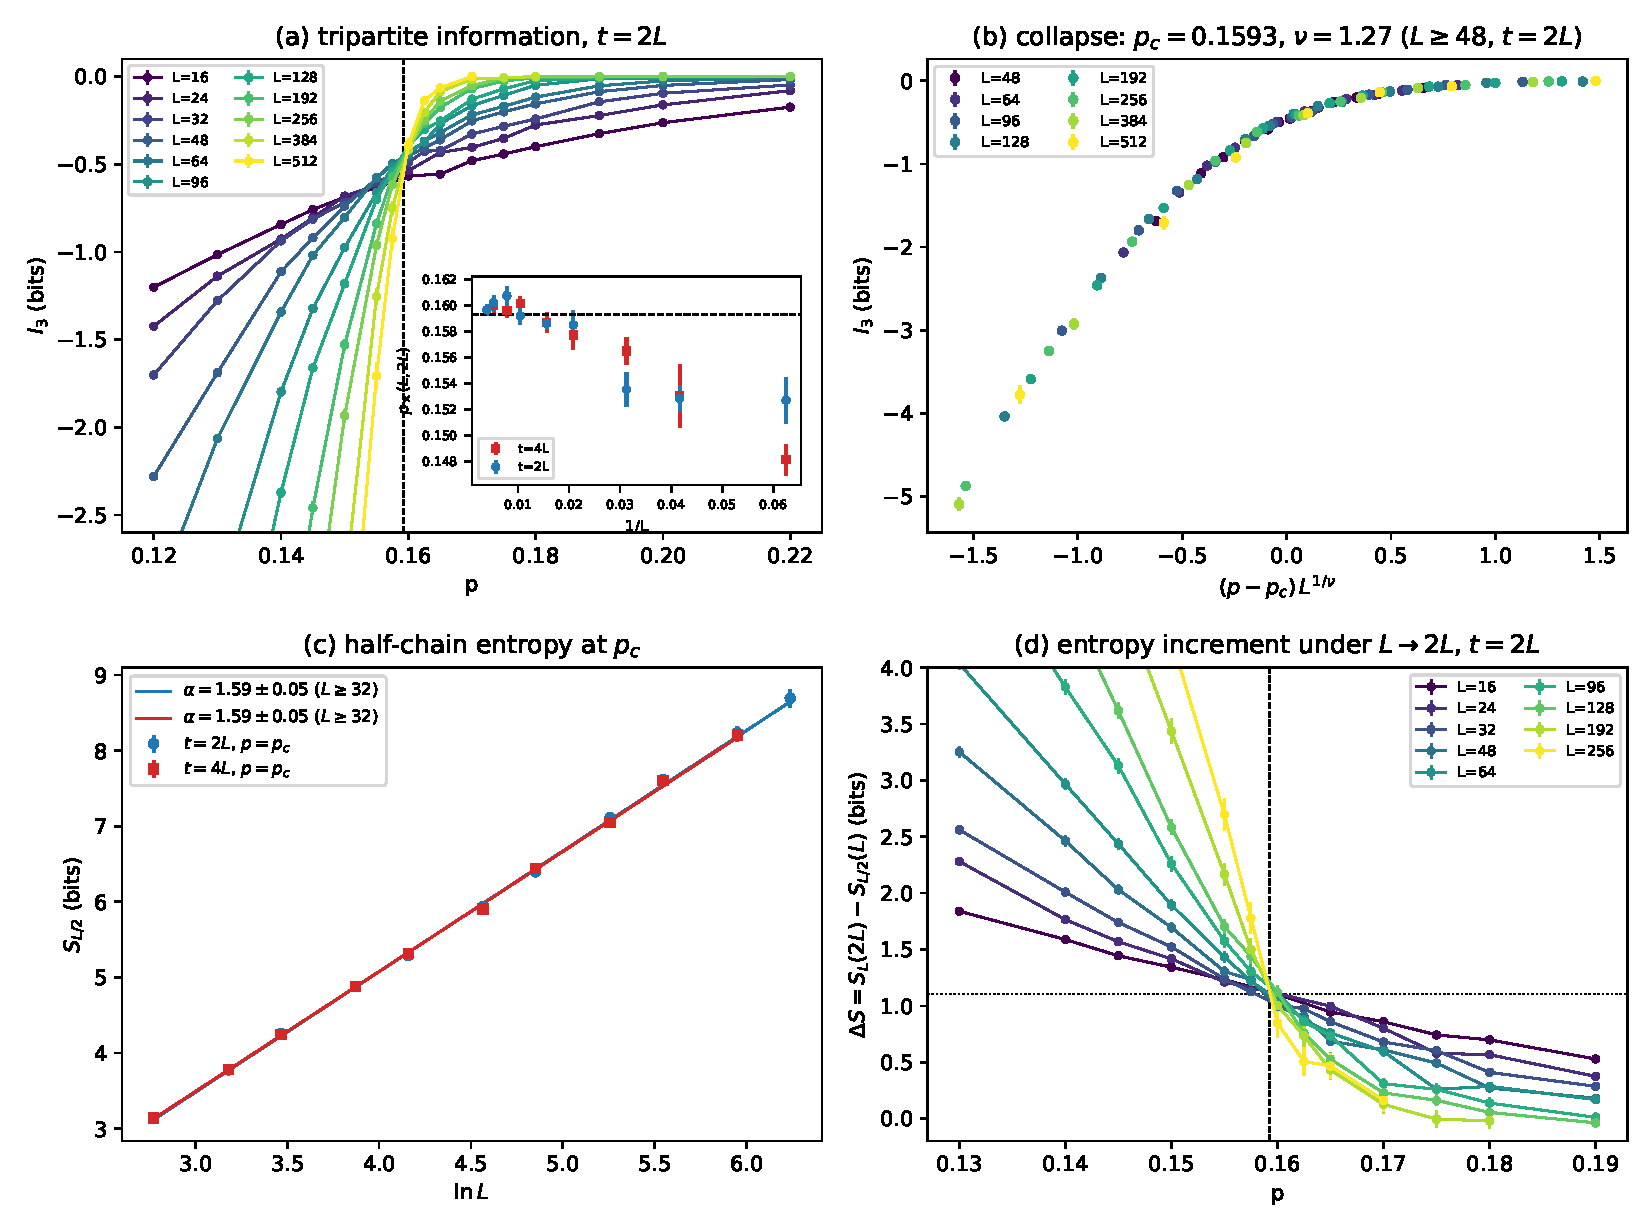
\includegraphics[width=\textwidth]{fig_final_fss_v16.pdf}
\caption{Quenched Clifford transition, $t=2L$.  (a) $I_3(p)$ for $L=16$--$512$; dashed line $p_c=0.1593$ from the collapse in (b); inset: crossings $p_\times(L,2L)$ (PCHIP estimator) against $1/L$ at $t=2L$ (circles) and $t=4L$ (squares).  (b) Collapse $I_3=F((p-p_c)L^{1/\nu})$, $L\ge48$, $|x|\le1.6$ shown.  (c) $S_{L/2}$ at $p_c$ (spline-interpolated in $p$) against $\ln L$ at $t=2L$ and $4L$ with the $L\ge32$ fits.  (d) Entropy increment $\Delta S=S_{L/2}(2L)-S_{L/2}(L)$; at $p_c$ it equals $\alpha\ln2$ (dotted) independently of $L$.}
\label{fig:numerics}
\end{figure*}

\emph{Critical point.}  Table~\ref{tab:numerics} lists the crossings of $I_3(L)$ and $I_3(2L)$ (monotone piecewise-cubic interpolation of each curve; three other estimators agree within $0.001$ for $L\ge96$).  They drift upward from $0.148$ at $L=16$ and saturate for $L\ge96$ at $0.1596$--$0.1607$ at both depths; a power-law extrapolation $p_\times=p_c+aL^{-\omega}$ gives $0.1602(6)$ ($\omega_{\rm eff}=1.6(4)$--$2.5(8)$ depending on $L_{\min}$) and the weighted plateau of the $L\ge96$ crossings $0.1599(3)$.  The joint collapse $I_3=F((p-p_c)L^{1/\nu})$ with a quartic $F$ on $|(p-p_c)L^{1/\nu}|\le1$ gives $p_c=0.1589$--$0.1595$, rising monotonically with the smallest size retained and stable against the window ($\pm0.0003$ for $|x|_{\max}\in\{0.6,1,1.5\}$), with $\chi^2/{\rm dof}=0.7$--$1.2$ for $L\ge64$ and $|x|_{\max}\le1$ ($\chi^2$ $p$-values $0.19$--$0.84$; $p\ge0.40$ for $|x|_{\max}=0.6$; the widest windows $|x|_{\max}=1.5$ reach $\chi^2/{\rm dof}=1.5$--$2.0$, $p=8\times10^{-6}$--$0.02$, through area-law-edge points).  The crossings of $\Delta S(L)=S_{L/2}(2L)-S_{L/2}(L)$ with $\Delta S(2L)$, an observable independent of $I_3$, give $0.159$--$0.161$ for $L\ge32$.  The entropy itself locates the same point once its non-universal part is handled correctly.  A collapse of the difference $S_{L/2}(p,L)-S_{L/2}(p_c,L)=G((p-p_c)L^{1/\nu})$ in the form of Ref.~\cite{Li2019} is unstable here ($p_c=0.1556$--$0.1638$, $\nu=1.0$--$1.27$ depending on the window and on a cut in the scaling variable), and the reason is identifiable: besides $\alpha\ln L+b$ the entropy contains an analytic, $L$-independent, cut-local term $a_1(p-p_c)$ with $a_1=+8$ to $+14$ bits per unit $p$ for two cuts (it doubles for the four-cut $S_{AC}$ and vanishes for the zero-net-cut combinations $I_3$, $S_{L/2}-S_{L/4}$ and $I(A{:}C)$); the subtraction at the fitted $p_c$ does not remove it, and a polynomial $G$ can absorb an $L$-independent tilt only by lowering $\nu$ and shifting $p_c$, producing a diagonal $\chi^2$ valley with ${\rm d}\nu/{\rm d}p_c\approx30$ in the $(p_c,\nu)$ plane.  Synthetic data generated from the pure scaling form do not show the instability; synthetic data with the fitted $a_1$ reproduce it.  Estimators in which the term cancels identically or is modelled give stable results: the collapses of $D=S_{L/2}-S_{L/4}$ and of $\Delta S_L=S_{L/2}(2L)-S_{L/2}(L)$ (no subtraction) give $p_c=0.1596$--$0.1602$, $\nu=1.21$--$1.25$ (bootstrap $\pm0.0004$, $\pm0.08$; $\chi^2/{\rm dof}=0.9$--$1.2$), and the joint fit $S_{L/2}=\alpha\ln L+b+a_1(p-p_c)+F((p-p_c)L^{1/\nu})$ over all depths, size cuts $L\ge32,48,64$, quartic or sextic $F$, with or without a cut, gives $p_c=0.1598$--$0.1601$ ($\pm0.0003$), $\nu=1.20$--$1.25$ ($\pm0.02$--$0.04$), $\chi^2/{\rm dof}=0.94$--$1.16$; omitting $a_1$ raises $\chi^2$ by $30$--$155$ for one degree of freedom and biases $\nu$ down to $1.08$--$1.16$, which is the bias of the subtracted form.  Adopted: $p_c=0.1597\pm0.0008$, the interval covering all estimators (the corrected, tail-safe fixed-set fits centre at $0.1597$--$0.1598$; the statistical errors alone are $\pm0.0003$).

\emph{Exponent.}  The collapse gives $\nu=1.18$--$1.27$ over all depth, size and window choices with $L\ge48$; the slope method $\partial_pI_3|_{p_c}\propto L^{1/\nu}$ (cubic fits over $|p-p_c|\le0.011$, $L=32$--$512$) gives $\nu=1.13$--$1.36$ as the assumed $p_c$ ranges over $0.1585$--$0.1605$; with $\nu$ frozen on \emph{fixed} point sets ($L\ge64$; spline scaling function with the area-law tail retained, over the eight tail-safe variants of the deposited report), the $\Delta\chi^2$ profiles are $52$--$334$ for $\nu=1$, $0.2$--$11$ for $\nu=1.20$, $0.1$--$2.6$ for $\nu=1.24$, $0$--$9.9$ for $\nu=1.28$, $3.0$--$36.5$ for $4/3$, and $12.5$--$89$ for $\nu=1.40$ (sextic scaling function with the tail removed: $\Delta\chi^2(\nu=1)\ge72$).  A power-law correction to scaling $AL^{-\omega}$ is preferred only when $L=48$ is retained ($\Delta\mathrm{AIC}=-7$ to $-14$), is neutral at $L\ge64$ and disfavoured at $L\ge96$, with $\omega$ undetermined ($0.3$--$4$, bootstrap s.e.\ $\approx1$); it raises $\nu$ by $0.02$--$0.04$.  We disclose the estimator weighting, whose defect biased earlier fixed-set fits: standard errors are floored at $1/N_{\rm traj}$ per point in the released code (the legacy $10^{-4}$/$10^{-6}$ floors of the v13 analysis code, which let a single saturated point---$I_3\equiv0$ in all $800$ trajectories at $L=384$, $p=0.18$---carry $98\%$ of one fixed-set fit's weight, are replaced by $1/N$), and the area-law points, which a polynomial scaling function cannot be flat on, are either removed or given a spline scaling function; the released pipeline, re-run on the recovered raw dataset, reproduces every windowed number of Table~\ref{tab:numerics} without change, confirming that no quoted window contains a floored point.  All $I_3$/entropy locators of this appendix share the same $475\,600$ trajectories; the only independent observable is the purification protocol below (disjoint seeds, mixed initial state).  Adopted: $\nu=1.24\pm0.07$, covering the full tail-safe envelope $1.21$--$1.29$; $\nu=1$ is excluded ($\Delta\chi^2\ge52$ in every variant), and the percolation value $4/3$ is disfavoured ($\Delta\chi^2\ge3$ in every variant, $\ge20$ without a correction term) but not excluded by the weakest variant.

\emph{Logarithmic entanglement.}  At $p_c$ (spline-interpolated in $p$, with the uncertainty of $p_c$ propagated) the half-chain entropy is linear in $\ln L$ from $L=16$ to $512$ with $\chi^2/{\rm dof}\le1.4$ (Table~\ref{tab:numerics}); at the neighbouring grid points $p=0.1575$ and $0.1625$ a straight line in $\ln L$ fails ($\chi^2/{\rm dof}=6$--$8$).  The straight-line fits give $\alpha=1.58$--$1.66$ at $p_c=0.1595$ but inherit ${\rm d}\alpha/{\rm d}p\approx-110$ times the uncertainty of $p_c$; the joint fit above, which determines $\alpha$ together with $p_c$, $\nu$ and the analytic background, gives $\alpha=1.50$--$1.56$ (bootstrap $\pm0.02$--$0.04$); a power-law correction $s_1L^{-y}$ ($y=\tfrac12,1,2$) is at most weakly preferred ($\Delta\mathrm{AIC}\ge-3$) and moves $\alpha$ by at most $0.14$; and the straight-line rows re-evaluated at the adopted $p_c=0.1597$ (spline window $p\in[0.145,0.175]$) give $\alpha=1.53$--$1.59$, inside the adopted interval, and the zero-net-cut collapses give $1.46$--$1.66$ through $F(0)$.  Adopted: $\alpha=1.55\pm0.07$ bits per $\ln L$ for the periodic half chain, i.e.\ $0.78(4)$ bits $=0.54(2)$ nats per entanglement cut, the interval covering all three routes.  Chord fits $S_\ell=a\ln[(L/\pi)\sin(\pi\ell/L)]+b$ to the four block sizes at fixed $L$ give $a=1.48$--$1.62$ bits for every $L$ from $64$ to $384$, and the mutual information of two antipodal quarters is $L$-independent at $p=0.16$ ($0.67(3)$, $0.73(4)$, $0.58(5)$, $0.69(7)$, $0.85(17)$ bits for $L=32,\dots,512$) while it grows at $p=0.155$ and decays at $p=0.165$, as conformal invariance requires.  In separate time-resolved runs at $p=0.16$ ($L=128,256,512$; $3000,1500,500$ trajectories; $t=1,2,4,\dots$) the growth before saturation is $S_{L/2}(t)=\alpha_t\ln t+{\rm const}$ with $\alpha_t=1.41(2)$, $1.44(2)$, $1.49(3)$ bits, the three sizes falling on one curve until each saturates at $t\approx L$; hence $z=\alpha/\alpha_t=1.03$--$1.10$, consistent with $z=1$ up to the same finite-size systematics.  In the boundary-CFT language of Ref.~\cite{Li2021}, $0.54(2)$ nats per cut is the scaling dimension $h_{a|b}$ of the entanglement boundary-condition-changing operator (their $0.53$); it is not a central charge.

\emph{Annealed versus quenched.}  The exact annealed quasi-entropy $\tilde S_2(A)$ of Eq.~\eqref{eq:collision} in the stationary Perron state exceeds the quenched $\E_\omega S(A)$ at every size and $p$; the excess is a change-of-measure effect rather than a convexity one: the record-collision weight of the annealed channel, proportional to $p_R^2$, favours records with fewer measurements and lowers the effective monitoring rate to $p_{\rm eff}=p+\frac{p(1-p)}{2L}\partial_p\ln\lambda_1$ ($0.105$ at $L=8$, $0.101$ at $L=12$, $0.092$ in the $L\to\infty$ limit at $p=0.16$; $0.149$ at $p_c^{(2)}$).  At $L=8$, $t=4$, $p=0.16$ ($40\,000$ Born trajectories, effective sample size $5935$): $\E_{\rm Born}S=2.019(4)$, $\E_{\rm Born}S(p_{\rm eff})=2.339(4)$, $\E_{\rm tilt}S=2.429$, exact $\tilde S_2=2.155$ bits---the density shift alone accounts for ${\approx}80\%$ of the tilt gain $\E_{\rm tilt}S-\E_{\rm Born}S(p)=0.41$ bits, of which Jensen removes $0.27$ bits, leaving the observed excess $\tilde S_2-\E_{\rm Born}S=0.14$ bits; at $L=12$ ($2.394(5)$, $2.941(4)$, $\tilde S_2=3.128$) the ordering is the same (the sampled tilt average there, effective sample size $454$, is not reliable and is not used).  The ratio growing from $1.3$ at $L=16$ to $1.8$ at $L=32$ for $p\in[0.16,0.22]$; $\tilde S_2$ grows linearly with $L$ for every $p<p_c^{(2)}$ (slope $\approx0.1$ bits per site at $p=0.22$), where the quenched entropy has already saturated at $\approx2.6$ bits with $I_3=0$.  The quenched transition at $0.1595$ and the annealed one at $0.2338$ are therefore distinct singularities of distinct quantities, as Sec.~\ref{sec:ising} states, and nothing quenched happens at $p_c^{(2)}$.  Haar-gate statevector runs with Born sampling ($L=8,12,16$) show the same ordering of annealed and quenched entropies, but these sizes are too small for an independent Haar transition point; the Haar values $p_c^{\rm H}=0.17(1)$, $\nu^{\rm H}=1.2(2)$ are those of Ref.~\cite{Zabalo2020}.

\emph{Comparison.}  For stabilizer circuits with the same Poissonian measurements the literature gives $p_c=0.16$, $\nu=1.3$, $\alpha=1.6$ bits~\cite{Li2019}; $p_c=0.154(4)$ ($L\le24$), $\nu=1.24(7)$, $z=1.06(4)$~\cite{Zabalo2020}; and $p_c=0.15995(10)$~\cite{Sierant2022}.  Gullans and Huse~\cite{Gullans2020} report $p_c=0.1593(5)$, $\nu=1.28(2)$; the coefficient $\tilde c\approx1.5$--$1.6$ quoted in that literature equals our $\alpha$ in units of $\ln2$.  The present values agree with all of them within the stated uncertainties.

\emph{Independent purification locator.}  A locator based on a different observable, and on trajectories disjoint from the $475\,600$ above, is the Gullans--Huse reference-qubit protocol~\cite{Gullans2020}: the $L$-qubit system starts completely mixed, purified by $L$ reference qubits ($2L$ qubits in total), and the same circuit and measurements act on the system only, so that $S_{\rm ref}(t)$, the entropy of the reference, is the entropy of the system's mixed state.  We ran $L=16$--$256$, $p=0.140$--$0.180$ (step $0.005$), $2000$--$4000$ trajectories per point (independent seeds), recording $S_{\rm ref}$ at $\tau=t/L=0.25,0.5,1,2,4$: $135\,000$ trajectories, $270$ files.  Sanity checks: $S_{\rm ref}=L$ at $p=0$; $S_{\rm ref}=0$ after one layer at $p=1$; $S_{\rm ref}\equiv S_{\rm sys}$ exactly; $N_{\rm meas}\approx2pLt$.  At $p=0.16$ the reference entropy is $L$-independent for $\tau\ge0.5$ ($\tau=1$: $1.72$, $1.75$, $1.77$ bits at $L=64,128,256$; $\tau=2$: $0.60$--$0.62$), i.e.\ a zero scaling dimension with $F(0,\tau)\sim1/\tau$.  Pair crossings of the $L\ge64$ curves give $0.1606$--$0.1628$; the collapses $S_{\rm ref}=F((p-p_c)L^{1/\nu})$ with a sextic $F$, $L\ge64$, give $p_c=0.1604$, $\nu=1.251$ ($\chi^2/{\rm dof}=15.5/18$) at $\tau=0.5$ and $p_c=0.1601$, $\nu=1.249$ ($18.3/18$) at $\tau=1$; a trajectory bootstrap ($100$ resamples) gives $0.16011(9)$, $1.250(14)$ at $\tau=1$.  The $\tau=2$ collapse ($0.1603$, $1.310$, $82.8/18$) is degraded by the same saturated-tail pathology as the fixed-set $I_3$ fits and is not used.  Frozen-$\nu$ $\Delta\chi^2$ on the $\tau=1$, $L\ge64$ set: $544$ ($\nu=1$), $16.9$ ($1.2$), $0.5$ ($1.24$), $6.6$ ($1.28$), $45.8$ ($4/3$), $139$ ($1.4$).  Hence $p_c^{\rm purif}=0.1601$--$0.1604$, $\nu^{\rm purif}=1.25(2)_{\rm stat}(6)_{\rm sys}$---an independent-observable confirmation of the $I_3$ headline, quoted separately and not entering the adopted $p_c=0.1597(8)$ (different observable, different finite-size corrections; combining them would hide that).  The purification analysis was re-run on the recovered dataset and reproduces every deposited number, the bootstrap values included, to the bit.

\begin{table}[t]
\caption{Finite-size-scaling summary for the quenched Clifford transition (bits; bootstrap errors in the last digits).  Top: crossings $p_\times(L,2L)$ of $I_3$.  Middle: collapse $I_3=F((p-p_c)L^{1/\nu})$ on $|x|\le1$ (bootstrap error of $p_c$ is $0.0001$--$0.0002$ in every row, from $200$ trajectory resamples ($100$ for the purification locator); standard errors are floored at $1/N_{\rm traj}$ per point in the released code, which moves no windowed number; the spread across rows is the systematic error; $\chi^2/{\rm dof}=2.2,1.6,1.1,0.7$ and $2.6,1.5,1.2,1.1$ down the two columns).  Bottom: slope $\alpha$ of $S_{L/2}$ against $\ln L$ at $p_c=0.1595$ (straight-line fits) and from the joint fit $\alpha\ln L+b+a_1(p-p_c)+F(x)$ with $p_c$, $\nu$, $a_1$ free (sextic $F$, no cut).  Last block: exact annealed $\tilde S_2$ against quenched $\E S_{L/2}$ at $t=2L$; the two columns are $p=0.16$ and $p=0.22$.}
\label{tab:numerics}
\begin{ruledtabular}
\begin{tabular}{lcc}
 & $t=4L$ & $t=2L$ \\
\colrule
\multicolumn{3}{l}{crossings $p_\times(L,2L)$ of $I_3$} \\
$(16,32)$ & 0.1481(12) & 0.1527(18) \\
$(24,48)$ & 0.1530(24) & 0.1529(10) \\
$(32,64)$ & 0.1565(10) & 0.1535(13) \\
$(48,96)$ & 0.1577(11) & 0.1585(11) \\
$(64,128)$ & 0.1587(7) & 0.1586(5) \\
$(96,192)$ & 0.1602(5) & 0.1592(7) \\
$(128,256)$ & 0.1596(5) & 0.1607(7) \\
$(192,384)$ & 0.1600(5) & 0.1602(6) \\
$(256,512)$ & -- & 0.1596(4) \\
\colrule
\multicolumn{3}{l}{collapse of $I_3$: $p_c$, $\nu$} \\
\multicolumn{3}{l}{purification locator ($\tau=1$, $L\ge64$, independent seeds): $0.1601$, $1.25(2)$} \\
$L\ge32$ & 0.1589, 1.23(1) & 0.1590, 1.26(1) \\
$L\ge48$ & 0.1591, 1.23(2) & 0.1593, 1.27(2) \\
$L\ge64$ & 0.1594, 1.18(3) & 0.1595, 1.26(4) \\
$L\ge96$ & 0.1595, 1.10(7) & 0.1594, 1.20(4) \\
\colrule
\multicolumn{3}{l}{$\alpha$ from $S_{L/2}=\alpha\ln L+b$ at $p_c$} \\
$L\ge16$ & 1.583(38) & 1.586(34) \\
$L\ge32$ & 1.586(51) & 1.595(52) \\
$L\ge48$ & 1.602(65) & 1.622(65) \\
$L\ge64$ & 1.630(66) & 1.657(70) \\
joint fit, $L\ge48$ & 1.519(33) & 1.509(26) \\
\colrule
\multicolumn{3}{l}{annealed $\tilde S_2$ / quenched $\E S_{L/2}$ ($t=2L$)} \\
$L=16$, $p=0.16$; $p=0.22$ & $4.13/3.13(2)$ & $3.10/2.30(2)$ \\
$L=32$, $p=0.16$; $p=0.22$ & $6.98/4.23(2)$ & $4.43/2.54(2)$ \\
\end{tabular}
\end{ruledtabular}
\end{table}

\begin{thebibliography}{99}
\bibitem{Li2018} Y.~Li, X.~Chen, and M.~P.~A.~Fisher, Phys. Rev. B \textbf{98}, 205136 (2018).
\bibitem{Skinner2019} B.~Skinner, J.~Ruhman, and A.~Nahum, Phys. Rev. X \textbf{9}, 031009 (2019).
\bibitem{Chan2019} A.~Chan, R.~M.~Nandkishore, M.~Pretko, and G.~Smith, Phys. Rev. B \textbf{99}, 224307 (2019).
\bibitem{Gullans2020} M.~J.~Gullans and D.~A.~Huse, Phys. Rev. X \textbf{10}, 041020 (2020).
\bibitem{Choi2020} S.~Choi, Y.~Bao, X.-L.~Qi, and E.~Altman, Phys. Rev. Lett. \textbf{125}, 030505 (2020).
\bibitem{Vasseur2019} R.~Vasseur, A.~C.~Potter, Y.-Z.~You, and A.~W.~W.~Ludwig, Phys. Rev. B \textbf{100}, 134203 (2019).
\bibitem{Jian2020} C.-M.~Jian, Y.-Z.~You, R.~Vasseur, and A.~W.~W.~Ludwig, Phys. Rev. B \textbf{101}, 104302 (2020).
\bibitem{Bao2020} Y.~Bao, S.~Choi, and E.~Altman, Phys. Rev. B \textbf{101}, 104301 (2020).
\bibitem{Houtappel1950} R.~M.~F.~Houtappel, Physica \textbf{16}, 425 (1950).
\bibitem{Li2019} Y.~Li, X.~Chen, and M.~P.~A.~Fisher, Phys. Rev. B \textbf{100}, 134306 (2019).
\bibitem{Zabalo2020} A.~Zabalo, M.~J.~Gullans, J.~H.~Wilson, S.~Gopalakrishnan, D.~A.~Huse, and J.~H.~Pixley, Phys. Rev. B \textbf{101}, 060301(R) (2020).
\bibitem{Cardy1986} J.~L.~Cardy, J.\ Phys.\ A \textbf{19}, L1093 (1986).
\bibitem{Wu1982} F.~Y.~Wu, Rev. Mod. Phys. \textbf{54}, 235 (1982); the exact $q=3$ exponents are $\nu=5/6$, $x_\sigma=2/15$, $x_\varepsilon=4/5$.
\bibitem{Sierant2022} P.~Sierant, M.~Schir\`o, M.~Lewenstein, and X.~Turkeshi, Phys. Rev. B \textbf{106}, 214316 (2022).
\bibitem{Kuo2020} W.-T.~Kuo, A.~A.~Akhtar, D.~P.~Arovas, and Y.-Z.~You, Phys. Rev. B \textbf{101}, 224202 (2020).
\bibitem{Collins2003} B.~Collins, Int. Math. Res. Not. \textbf{2003}, 953 (2003).
\bibitem{CollinsSniady2006} B.~Collins and P.~\'Sniady, Commun. Math. Phys. \textbf{264}, 773 (2006).
\bibitem{StewartSun1990} G.~W.~Stewart and J.-G.~Sun, \emph{Matrix Perturbation Theory} (Academic Press, Boston, 1990).
\bibitem{Brandao2016} F.~G.~S.~L.~Brand\~ao, A.~W.~Harrow, and M.~Horodecki, Commun. Math. Phys. \textbf{346}, 397 (2016).
\bibitem{DiVincenzo2002} D.~P.~DiVincenzo, D.~W.~Leung, and B.~M.~Terhal, IEEE Trans. Inf. Theory \textbf{48}, 580 (2002).
\bibitem{Watrous2018} J.~Watrous, \emph{The Theory of Quantum Information} (Cambridge University Press, Cambridge, 2018).
\bibitem{Sylvester1851} J.~J.~Sylvester, Philos. Mag. \textbf{1}, 295 (1851).
\bibitem{HornJohnson2013} R.~A.~Horn and C.~R.~Johnson, \emph{Matrix Analysis}, 2nd ed. (Cambridge University Press, Cambridge, 2013).
\bibitem{Flanders1951} H.~Flanders, Proc. Am. Math. Soc. \textbf{2}, 871 (1951).
\bibitem{Baxter1982} R.~J.~Baxter, \emph{Exactly Solved Models in Statistical Mechanics} (Academic Press, London, 1982).
\bibitem{Ruelle1969} D.~Ruelle, \emph{Statistical Mechanics: Rigorous Results} (W. A. Benjamin, New York, 1969).
\bibitem{Kaufman1949} B.~Kaufman, Phys. Rev. \textbf{76}, 1232 (1949).
\bibitem{Newell1950} G.~F.~Newell, Phys. Rev. \textbf{79}, 876 (1950).
\bibitem{Schultz1964} T.~Schultz, D.~Mattis, and E.~Lieb, Rev. Mod. Phys. \textbf{36}, 856 (1964).
\bibitem{Stephenson1964} J.~Stephenson, J. Math. Phys. \textbf{5}, 1009 (1964).
\bibitem{Stephenson1970} J.~Stephenson, J. Math. Phys. \textbf{11}, 420 (1970).
\bibitem{Potts1952} R.~B.~Potts, Phys. Rev. \textbf{88}, 352 (1952).
\bibitem{Brylinski2002} J.-L.~Brylinski and R.~Brylinski, Universal quantum gates, in \emph{Mathematics of Quantum Computation}, edited by R.~K.~Brylinski and G.~Chen (Chapman \& Hall/CRC, Boca Raton, 2002); arXiv:quant-ph/0108062.
\bibitem{SM} See Supplemental Material at [URL will be inserted by publisher] for the exceptional-point tables of the three-replica compressed operator ($d=2,3$), the per-block certificate data at $L=12$, the endpoint and $p_\times$ ranks, and the complete list of certificate files with SHA-256 hashes and reproduction commands.
\bibitem{Shi2003} Y.~Shi, Quantum Inf. Comput. \textbf{3}, 84 (2003).
\bibitem{Aharonov2003} D.~Aharonov, arXiv:quant-ph/0301040 (2003).
\bibitem{Fenner1994} S.~A.~Fenner, L.~J.~Fortnow, and S.~A.~Kurtz, J. Comput. Syst. Sci. \textbf{48}, 116 (1994).
\bibitem{Aaronson2005} S.~Aaronson, Proc. R. Soc. A \textbf{461}, 3473 (2005).
\bibitem{NielsenChuang2010} M.~A.~Nielsen and I.~L.~Chuang, \emph{Quantum Computation and Quantum Information}, 10th anniversary ed. (Cambridge University Press, Cambridge, 2010).
\bibitem{DelMoral2004} P.~Del~Moral, \emph{Feynman--Kac Formulae: Genealogical and Interacting Particle Systems with Applications} (Springer, New York, 2004).
\bibitem{FurstenbergKesten1960} H.~Furstenberg and H.~Kesten, Ann. Math. Stat. \textbf{31}, 457 (1960).
\bibitem{Ruelle1979} D.~Ruelle, Adv. Math. \textbf{32}, 68 (1979).
\bibitem{Peres1992} Y.~Peres, Ann. Inst. H. Poincar\'e Probab. Statist. \textbf{28}, 131 (1992).
\bibitem{DemboZeitouni1998} A.~Dembo and O.~Zeitouni, \emph{Large Deviations Techniques and Applications}, 2nd ed. (Springer, New York, 1998).
\bibitem{Derrida1981} B.~Derrida, Phys. Rev. B \textbf{24}, 2613 (1981).
\bibitem{BLM2013} S.~Boucheron, G.~Lugosi, and P.~Massart, \emph{Concentration Inequalities: A Nonasymptotic Theory of Independence} (Oxford University Press, Oxford, 2013).
\bibitem{Rockafellar1970} R.~T.~Rockafellar, \emph{Convex Analysis} (Princeton University Press, Princeton, 1970).
\bibitem{Giardina2006} C.~Giardin\`a, J.~Kurchan, and L.~Peliti, Phys. Rev. Lett. \textbf{96}, 120603 (2006).
\bibitem{Tailleur2009} J.~Tailleur and V.~Lecomte, AIP Conf. Proc. \textbf{1091}, 212 (2009).
\bibitem{Gantmacher1959} F.~R.~Gantmacher, \emph{The Theory of Matrices}, Vol.~1 (Chelsea, New York, 1959).
\bibitem{Li2021} Y.~Li, X.~Chen, A.~W.~W.~Ludwig, and M.~P.~A.~Fisher, Phys. Rev. B \textbf{104}, 104305 (2021).
\end{thebibliography}

\end{document}
